% -*- Mode:TeX -*-

%% IMPORTANT: The official thesis specifications are available at:
%%            http://libraries.mit.edu/archives/thesis-specs/
%%
%%            Please verify your thesis' formatting and copyright
%%            assignment before submission.  If you notice any
%%            discrepancies between these templates and the 
%%            MIT Libraries' specs, please let us know
%%            by e-mailing thesis@mit.edu

%% The documentclass options along with the pagestyle can be used to generate
%% a technical report, a draft copy, or a regular thesis.  You may need to
%% re-specify the pagestyle after you \include  cover.tex.  For more
%% information, see the first few lines of mitthesis.cls. 

\documentclass[12pt,twoside]{mitthesis}
%%
%%  If you want your thesis copyright to you instead of MIT, use the
%%  ``vi'' option, as above.
%%
%\documentclass[12pt,twoside,leftblank]{mitthesis}
%%
%% If you want blank pages before new chapters to be labelled ``This
%% Page Intentionally Left Blank'', use the ``leftblank'' option, as
%% above. 

%\documentclass[12pt,twoside]{mitthesis}
%\usepackage{times}
\usepackage{lgrind}
%% These have been added at the request of the MIT Libraries, because
%% some PDF conversions mess up the ligatures.  -LB, 1/22/2014
\usepackage{cmap}
\usepackage[T1]{fontenc}
\pagestyle{plain}

%% This bit allows you to either specify only the files which you wish to
%% process, or `all' to process all files which you \include.
%% Krishna Sethuraman (1990).

%\typein [\files]{Enter file names to process, (chap1,chap2 ...), or `all' to
%process all files:}
%\def\all{all}
%\ifx\files\all \typeout{Including all files.} \else \typeout{Including only \files.} \includeonly{\files} \fi

\begin{document}

% -*-latex-*-
% 
% For questions, comments, concerns or complaints:
% thesis@mit.edu
% 
%
% $Log: cover.tex,v $
% Revision 1.8  2008/05/13 15:02:15  jdreed
% Degree month is June, not May.  Added note about prevdegrees.
% Arthur Smith's title updated
%
% Revision 1.7  2001/02/08 18:53:16  boojum
% changed some \newpages to \cleardoublepages
%
% Revision 1.6  1999/10/21 14:49:31  boojum
% changed comment referring to documentstyle
%
% Revision 1.5  1999/10/21 14:39:04  boojum
% *** empty log message ***
%
% Revision 1.4  1997/04/18  17:54:10  othomas
% added page numbers on abstract and cover, and made 1 abstract
% page the default rather than 2.  (anne hunter tells me this
% is the new institute standard.)
%
% Revision 1.4  1997/04/18  17:54:10  othomas
% added page numbers on abstract and cover, and made 1 abstract
% page the default rather than 2.  (anne hunter tells me this
% is the new institute standard.)
%
% Revision 1.3  93/05/17  17:06:29  starflt
% Added acknowledgements section (suggested by tompalka)
% 
% Revision 1.2  92/04/22  13:13:13  epeisach
% Fixes for 1991 course 6 requirements
% Phrase "and to grant others the right to do so" has been added to 
% permission clause
% Second copy of abstract is not counted as separate pages so numbering works
% out
% 
% Revision 1.1  92/04/22  13:08:20  epeisach

% NOTE:
% These templates make an effort to conform to the MIT Thesis specifications,
% however the specifications can change.  We recommend that you verify the
% layout of your title page with your thesis advisor and/or the MIT 
% Libraries before printing your final copy.
\title{\textsc{Designing fast and programmable routers}}

\author{\textsc{Anirudh Sivaraman Kaushalram}}
% If you wish to list your previous degrees on the cover page, use the 
% previous degrees command:
%       \prevdegrees{A.A., Harvard University (1985)}
% You can use the \\ command to list multiple previous degrees
       \prevdegrees{
\begin{tabular}{rll}
Master of Science, & \hspace{-9 pt}Massachusetts Institute of Technology (2012) \\
Bachelor of Technology, & \hspace{-9 pt}Indian Institute of Technology Madras (2010) \\
\end{tabular}}

\department{\mbox{Department of Electrical Engineering and Computer Science}}

% If the thesis is for two degrees simultaneously, list them both
% separated by \and like this:
% \degree{Doctor of Philosophy \and Master of Science}
\degree{Doctor of Philosophy}

% As of the 2007-08 academic year, valid degree months are September, 
% February, or June.  The default is June.
\degreemonth{September}
\degreeyear{2017}
\thesisdate{August 31, 2017}

%% By default, the thesis will be copyrighted to MIT.  If you need to copyright
%% the thesis to yourself, just specify the `vi' documentclass option.  If for
%% some reason you want to exactly specify the copyright notice text, you can
%% use the \copyrightnoticetext command.  
%\copyrightnoticetext{\copyright IBM, 1990.  Do not open till Xmas.}

% If there is more than one supervisor, use the \supervisor command
% once for each.
\supervisor{Hari Balakrishnan}{Fujitsu Chair Professor}
\supervisor{Mohammad Alizadeh}{TIBCO Career Development Assistant Professor}

% This is the department committee chairman, not the thesis committee
% chairman.  You should replace this with your Department's Committee
% Chairman.
\chairman{Leslie A.~Kolodziejski}{Professor of Electrical Engineering\\ Chair, Department Committee on Graduate Students}

% Make the titlepage based on the above information.  If you need
% something special and can't use the standard form, you can specify
% the exact text of the titlepage yourself.  Put it in a titlepage
% environment and leave blank lines where you want vertical space.
% The spaces will be adjusted to fill the entire page.  The dotted
% lines for the signatures are made with the \signature command.
\maketitle

% The abstractpage environment sets up everything on the page except
% the text itself.  The title and other header material are put at the
% top of the page, and the supervisors are listed at the bottom.  A
% new page is begun both before and after.  Of course, an abstract may
% be more than one page itself.  If you need more control over the
% format of the page, you can use the abstract environment, which puts
% the word "Abstract" at the beginning and single spaces its text.

%% You can either \input (*not* \include) your abstract file, or you can put
%% the text of the abstract directly between the \begin{abstractpage} and
%% \end{abstractpage} commands.

% First copy: start a new page, and save the page number.
\cleardoublepage
% Uncomment the next line if you do NOT want a page number on your
% abstract and acknowledgments pages.
% \pagestyle{empty}
\setcounter{savepage}{\thepage}
\begin{abstractpage}
% $Log: abstract.tex,v $
% Revision 1.1  93/05/14  14:56:25  starflt
% Initial revision
% 
% Revision 1.1  90/05/04  10:41:01  lwvanels
% Initial revision
% 
%
%% The text of your abstract and nothing else (other than comments) goes here.
%% It will be single-spaced and the rest of the text that is supposed to go on
%% the abstract page will be generated by the abstractpage environment.  This
%% file should be \input (not \include 'd) from cover.tex.
Historically, the evolution of network routers was driven primarily by
performance. Recently, owing to the need for better control over network
operations and the constant demand for new features, programmability of routers
has become as important as performance.  However, today's fastest routers,
which have 10--100 ports each running at a line rate of 10--100 Gbit/s, use
fixed-function hardware, which cannot be modified after deployment. This
dissertation describes three router hardware primitives and their
corresponding software programming models that allow network operators to
program specific classes of router functionality on such fast routers.

First, we develop a system for programming stateful packet-processing
algorithms such as algorithms for in-network congestion control, buffer
management, and data-plane traffic engineering. The challenge here is the fact
that these algorithms maintain and update state on the router.  We develop a
small but expressive instruction set for state manipulation on fast routers.
 We then expose this to the programmer through a high-level programming model
and compiler.

Second, we develop a system to program packet scheduling: the task of picking
which packet to transmit next on a link. Our main contribution here is the
finding that many packet scheduling algorithms can be programmed using one
simple idea: a priority queue of packets in hardware coupled with a software
program to assign each packet's priority in this queue.

Third, we develop a system for programmable and scalable measurement of network
statistics. Our goal is to allow programmers to flexibly define what they want
to measure for each flow and scale to a large number of flows. We formalize
a class of statistics that permit a scalable
implementation and show that it includes many useful statistics (\eg
moving averages and counters).

These systems show that it is possible to program several packet-processing
functions at speeds approaching today's fastest routers. Based on these systems, we
distill two lessons for designing fast and programmable routers in the future.
First, specialized designs that program only specific classes of router
functionality improve packet processing throughput by 10--100x relative to a general-purpose
solution. Second, joint design of
hardware and software provides us with more leverage relative to designing only
one of them while keeping the other fixed.

% Try and mention compiler and vertical integration here (and if so), then
% also bring them up in the main text.

\end{abstractpage}

\newpage \vspace*{8cm}
% Sets a PDF bookmark for the dedication
\pdfbookmark{Dedication}{dedication}
\thispagestyle{empty}
\begin{center}
  \Large \emph{To my grandfather, the late Dr. V. Ramamurti}
\end{center}

% Additional copy: start a new page, and reset the page number.  This way,
% the second copy of the abstract is not counted as separate pages.
% Uncomment the next 6 lines if you need two copies of the abstract
% page.
% \setcounter{page}{\thesavepage}
% \begin{abstractpage}
% % $Log: abstract.tex,v $
% Revision 1.1  93/05/14  14:56:25  starflt
% Initial revision
% 
% Revision 1.1  90/05/04  10:41:01  lwvanels
% Initial revision
% 
%
%% The text of your abstract and nothing else (other than comments) goes here.
%% It will be single-spaced and the rest of the text that is supposed to go on
%% the abstract page will be generated by the abstractpage environment.  This
%% file should be \input (not \include 'd) from cover.tex.
Historically, the evolution of network routers was driven primarily by
performance. Recently, owing to the need for better control over network
operations and the constant demand for new features, programmability of routers
has become as important as performance.  However, today's fastest routers,
which have 10--100 ports each running at a line rate of 10--100 Gbit/s, use
fixed-function hardware, which cannot be modified after deployment. This
dissertation describes three router hardware primitives and their
corresponding software programming models that allow network operators to
program specific classes of router functionality on such fast routers.

First, we develop a system for programming stateful packet-processing
algorithms such as algorithms for in-network congestion control, buffer
management, and data-plane traffic engineering. The challenge here is the fact
that these algorithms maintain and update state on the router.  We develop a
small but expressive instruction set for state manipulation on fast routers.
 We then expose this to the programmer through a high-level programming model
and compiler.

Second, we develop a system to program packet scheduling: the task of picking
which packet to transmit next on a link. Our main contribution here is the
finding that many packet scheduling algorithms can be programmed using one
simple idea: a priority queue of packets in hardware coupled with a software
program to assign each packet's priority in this queue.

Third, we develop a system for programmable and scalable measurement of network
statistics. Our goal is to allow programmers to flexibly define what they want
to measure for each flow and scale to a large number of flows. We formalize
a class of statistics that permit a scalable
implementation and show that it includes many useful statistics (\eg
moving averages and counters).

These systems show that it is possible to program several packet-processing
functions at speeds approaching today's fastest routers. Based on these systems, we
distill two lessons for designing fast and programmable routers in the future.
First, specialized designs that program only specific classes of router
functionality improve packet processing throughput by 10--100x relative to a general-purpose
solution. Second, joint design of
hardware and software provides us with more leverage relative to designing only
one of them while keeping the other fixed.

% Try and mention compiler and vertical integration here (and if so), then
% also bring them up in the main text.

% \end{abstractpage}

% Some departments (e.g. 5) require an additional signature page.  See
% signature.tex for more information and uncomment the following line if
% applicable.
% % -*- Mode:TeX -*-
%
% Some departments (e.g. Chemistry) require an additional cover page
% with signatures of the thesis committee.  Please check with your
% thesis advisor or other appropriate person to determine if such a 
% page is required for your thesis.  
%
% If you choose not to use the "titlepage" environment, a \newpage
% commands, and several \vspace{\fill} commands may be necessary to
% achieve the required spacing.  The \signature command is defined in
% the "mitthesis" class
%
% The following sample appears courtesy of Ben Kaduk <kaduk@mit.edu> and
% was used in his June 2012 doctoral thesis in Chemistry. 

\begin{titlepage}
\begin{large}
This doctoral thesis has been examined by a Committee of the Department
of Chemistry as follows:

\signature{Professor Jianshu Cao}{Chairman, Thesis Committee \\
   Professor of Chemistry}

\signature{Professor Troy Van Voorhis}{Thesis Supervisor \\
   Associate Professor of Chemistry}

\signature{Professor Robert W. Field}{Member, Thesis Committee \\
   Haslam and Dewey Professor of Chemistry}
\end{large}
\end{titlepage}


\pagestyle{plain}
  % -*- Mode:TeX -*-
%% This file simply contains the commands that actually generate the table of
%% contents and lists of figures and tables.  You can omit any or all of
%% these files by simply taking out the appropriate command.  For more
%% information on these files, see appendix C.3.3 of the LaTeX manual. 
\tableofcontents
%\newpage
%\listoffigures
%\newpage
%\listoftables

\chapter*{Previously Published Material}
\addcontentsline{toc}{chapter}{Previously Published Material}%

{
\setlength{\parindent}{0 pt}
\setlength{\parskip}{\baselineskip}

Chapter~\ref{chap:domino}~revises a previous
publication~\cite{domino_sigcomm}:
Anirudh Sivaraman, Alvin Cheung, Mihai Budiu, Changhoon Kim, Mohammad Alizadeh, Hari Balakrishnan, George Varghese, Nick McKeown, and Steve Licking.
\newblock{Packet Transactions: High-Level Programming for Line-Rate Switches}.
\newblock In {\em SIGCOMM}, Florianopolis, Brazil, August 2016.

Chapter~\ref{chap:pifo} combines material from two previous
publications~\cite{pifo_hotnets, pifo_sigcomm}:
\begin{CompactEnumerate}
\item
Anirudh Sivaraman, Suvinay Subramanian, Anurag Agrawal, Sharad Chole, Shang-Tse Chuang, Tom Edsall, Mohammad Alizadeh, Sachin Katti, Nick McKeown, and Hari Balakrishnan.
\newblock{Towards Programmable Packet Scheduling}.
\newblock In {\em HotNets}, Philadelphia, U.S.A, November 2015.

\item
Anirudh Sivaraman, Suvinay Subramanian, Mohammad Alizadeh, Sharad Chole, Shang-Tse Chuang, Anurag Agrawal, Hari Balakrishnan, Tom Edsall, Sachin Katti, and Nick McKeown.
\newblock {Programmable Packet Scheduling at Line Rate}.
\newblock In {\em SIGCOMM}, Florianopolis, Brazil, August 2016.
\end{CompactEnumerate}

Chapter~\ref{chap:perf_query}~revises a previous publication~\cite{perf_query}:
Srinivas Narayana, Anirudh Sivaraman, Vikram Nathan, Prateesh Goyal, Venkat Arun, Mohammad Alizadeh, Vimalkumar Jeyakumar, and Changhoon Kim.
\newblock {Language-Directed Hardware Design for Network Performance Monitoring
}.
\newblock In {\em SIGCOMM}, Los Angeles, U.S.A, August 2017.
}

\chapter*{Acknowledgments}
\addcontentsline{toc}{chapter}{Acknowledgements}%

In one sense, this thesis work has occupied a third of my
life---counting from when I became a graduate student in 2003, and
keeping the clock running for my sojourns away as I figured out what
to work on when I came back. Arriving at this point would have been
impossible without the help of a large number of people.

My advisor, Hari Balakrishnan, has been a tireless counselor, mentor,
booster, and co-author. I'm lucky to have had the benefit of his
wisdom, his nose for interesting problems, and his tendency to get
hooked and excited and to champion any idea that comes from his students.

I'm especially grateful to my frequent co-author and labmate, Anirudh
Sivaraman, who taught me how to be a productive collaborator, and
without whom most of this work could not have been realized.

Thank you to my thesis committee, of Hari Balakrishnan, Dina Katabi,
Scott Shenker, and Leslie Kaelbling, who have reached out across
disciplines to support and guide this work.

Just before I headed off to MIT as an undergraduate in 1999, I was
advised in strong terms to look up Gerald Jay Sussman when I got
there. I didn't know what I was in for! I have worked with Gerry since
I was a freshman and cannot easily express how much I have gained from
his mentorship, his knowledge, and his sense of taste.

My informal ``backup advisors'' on the ninth floor---Nickolai
Zeldovich and M.~Frans Kaashoek---have been patient through
innumerable practice talks and late-night idea-bouncing
sessions. Outside the ninth floor, I have been fortunate to have the
support and counsel of Victor Bahl, Hal Abelson, Jonathan Zittrain,
and Mike Walfish.

I owe much to my time in the Wall Street Journal's late Boston
bureau. My editors Gary Putka and Dan Golden, and my colleague Charles
Forelle, taught me how to develop a nose for investigations and how to
tell a story. Gary's ``dun-colored warren of cubicles'' represented a
journalistic Camelot and was as intellectually challenging as any lab
in academia.

Many others helped to develop the ideas in this work, especially
Pratiksha Thaker, Chris Amato, Andrew McGregor, Tim Shepard, John
Wroclawski, Bill McCloskey, Josh Mandel, Carrie Niziolek, Damon
Wischik, Hariharan Rahul, Chris Lesniewski, Vikash Mansinghka, Eric
Jonas, Marissa Cheng, and Allie Brownell.

To my labmates and ninth floor coinhabitants---Katrina LaCurts, Raluca
Ada Popa, Shuo Deng, Lenin Ravindranath, Ravi Netravali, Peter
Iannucci, Tiffany Chen, Amy Ousterhout, Jonathan Perry, Neha Narula,
Austin Clements, Cody Cutler, Eugene Wu, Dan Ports, and Sheila
Marian---thank you for your companionship and our time together.

Immeasurable gratitude is due to my mom, Joan Winstein, and my sister Allison,
for supporting and putting up with me and giving me a sense of how
things ought to be. To all our sadness, my father passed away just
after making it to Allison's master's recital and just after my return
to graduate school in 2011. When I was young, my dad would sometimes
bring home his graduate students in physics for dinner, some of whom
became surrogate older siblings for a time. Much later, for his
retirement, they all wrote about his incredible attention to detail
and his sense of right and wrong in constructing tests of Mother
Nature---things I have always admired and hope have partly
rubbed off on me.

When he died, the university was kind enough to let me ghostwrite his
obituary, and so my dad will always be remembered the way I saw
him. I'll add one more thing, by dedicating this dissertation to his
memory.

\chapter{Sprout: Explicit Forecasts of Future Network Capacity}
\label{chap:sprout}

\begin{abstract}
Sprout is an end-to-end transport protocol for interactive
applications that desire high throughput and low delay. Sprout works
well over cellular wireless networks, where link speeds change
dramatically with time, and current protocols build up multi-second
queues in network gateways. Sprout does not use TCP-style reactive
congestion control; instead the receiver observes the packet arrival
times to infer the uncertain dynamics of the network path. This
inference is used to forecast how many bytes may be sent by the
sender, while bounding the risk that packets will be delayed inside
the network for too long.

In evaluations on traces from four commercial LTE and 3G networks,
Sprout, compared with Skype, reduced self-inflicted end-to-end delay
by a factor of 7.9 and achieved 2.2$\times$ the transmitted bit rate
on average. Compared with Google's Hangout, Sprout reduced delay by a
factor of 7.2 while achieving 4.4$\times$ the bit rate, and compared
with Apple's Facetime, Sprout reduced delay by a factor of 8.7 with
1.9$\times$ the bit rate.

Although it is end-to-end, Sprout matched or outperformed TCP Cubic
running over the CoDel active queue management algorithm, which
requires changes to cellular carrier equipment to deploy. We also
tested Sprout as a tunnel to carry competing interactive and bulk
traffic (Skype and TCP Cubic), and found that Sprout was able to isolate
client application flows from one another.

\end{abstract}

%\section{Introduction}
\label{sprout:intro}

Cellular wireless networks have become a dominant mode of Internet
access. These mobile networks, which include LTE and 3G (UMTS and
1xEV-DO) services, present new challenges for network applications,
because they behave differently from wireless LANs and from the
Internet's traditional wired infrastructure.

Cellular wireless networks experience rapidly varying link rates
and occasional multi-second outages in one or both directions,
especially when the user is mobile. As a result, the time it takes to
deliver a network-layer packet may vary significantly, and may include
the effects of link-layer retransmissions. Moreover, these networks
schedule transmissions after taking channel quality into account, and
prefer to have packets waiting to be sent whenever a link is
scheduled. They often achieve that goal by maintaining deep packet
queues. The effect at the transport layer is that a stream of packets
experiences widely varying packet delivery rates, as well as variable,
sometimes multi-second, packet delays.


%To ameliorate these issues, these networks use semi-reliable protocols
%with link-layer retransmissions and enqueue packets waiting to be
%transmitted so that the link, when available, does not starve for
%packets.  As a result, these networks experience high variations in
%achievable transmission rates as well as packet delays.

For an interactive application such as a videoconferencing program
that requires both high throughput and low delay, these conditions are
challenging. If the application sends at too low a rate, it will waste
the opportunity for higher-quality service when the link is
doing well. But when the application sends too aggressively, it
accumulates a queue of packets inside the network waiting to be
transmitted across the cellular link, delaying subsequent
packets. Such a queue can take several seconds to drain, destroying
interactivity (see Figure~\ref{fig:skypevssprout}).

%Furthermore, even if the transport protocol knew the varying rate of
%the network path exactly, a videoconferencing application would not
%benefit unless it could rapidly adapt the quality of its video
%encoding to meet the available rate.  Unfortunately, this task is
%difficult and done poorly by existing videoconferencing
%applications. To match a time-varying rate, the application needs to
%control the coded size of each outgoing video frame. To help the
%client recover from loss, the application needs to ensure that
%transmitted video frames depend only on frames available to the
%receiver, and not frames that have been lost. Current video coder
%libraries generally don't expose this level of control to
%applications.

Our experiments with Microsoft's Skype, Google's Hangouts, and Apple's
Facetime running over traces from commercial 3G and LTE networks show
the shortcomings of the transport protocols in use and the lack of
adaptation required for a good user experience.
%(\S\ref{s:problem}). 
The transport protocols deal with rate variations in a reactive
manner: they attempt to send at a particular rate, and if all goes
well, they increase the rate and try again. They are slow to
decrease their transmission rate when the link has deteriorated, and as a
result they often create a large backlog of queued packets in the
network. When that happens, only after several seconds and a
user-visible outage do they switch to a lower rate.
%The
%encoder pre-determines which frames should be sent at any given
%encoding rate, not adapting to what the receiver might (or might not)
%have recently received.

%\subsection{Contributions}

\begin{figure}
\caption{Skype and Sprout on the emulated Verizon LTE downlink. For Skype, overshoots in throughput lead to large standing queues. Sprout tries to keep each
packet's delay less than 100~ms with 95\% probability.}
\label{fig:skypevssprout}
\vspace{\baselineskip}
\def\svgwidth{\columnwidth}\input{newfigure1.pdf_tex}
\end{figure}

%\paragraph{Contributions.}
This chapter describes Sprout, a transport protocol designed for
interactive applications on variable-quality networks. Sprout uses the
receiver's observed packet arrival times as the primary signal to
determine how the network path is doing, rather than the packet loss,
round-trip time, or one-way delay. Moreover, instead of the
traditional reactive approach where the sender's window or rate
increases or decreases in response to a congestion signal, the Sprout
receiver makes a short-term forecast (at times in the near future) of
the bottleneck link rate using probabilistic inference.  From this
model, the receiver predicts how many bytes are likely to cross the
link within several intervals in the near future with at least 95\%
probability. The sender uses this forecast to transmit its data,
bounding the risk that the queuing delay will exceed some threshold,
and maximizing the achieved throughput within that constraint.

%This is difficult for existing videoconferencing systems. To match the
%capacity of a varying link, the application needs to control the coded
%size of each outgoing video frame. To help the client recover from
%loss, the application needs to ensure that transmitted video frames
%depend only on frames available to the receiver (and not frames that
%have been lost). Current video coder libraries generally don't expose
%this level of control to calling applications.
%
%In our experiments using trace-based emulation of cellular networks,
%we have found that videoconferencing programs --- including
%Microsoft's Skype, Google's Hangout, and Apple's Facetime --- operate
%poorly over commercial 3G and LTE service. Based on our measurements,
%these programs deal with varying link speeds in a reactive manner.
%They attempt to send at a particular rate. If all goes well, after
%several seconds they increase the rate in a large jump and try
%again. If they are accumulating a large delay, again only after
%several seconds, and a user-visible outage, does the program switch to
%a lower rate.

%\begin{enumerate}a

%\item 


%  In practice, Sprout responds more quickly than existing schemes to
%  increases or decreases in path rates because it does not need to
%  wait for detectable changes in the observed round-trip time or for
%  losses. Scout generally achieves higher throughput and lower delay
%  than competing end-to-end schemes.

%  Sprout sends as much data as it can---subject to
%   the constraint that no outgoing packet will end up waiting behind
%   other packets in a network queue for more than 100
%   milliseconds. Sprout can't guarantee this, but it does its best to
%   bound the risk of violating the constraint at less than 5\% per
%   packet.

%  The Sprout receiver maintains a stochastic model of the cellular
%  link, and uses probabilistic inference to evolve a probability
%  density function on the network's underlying link speed. From this
%  probability distribution and model, Sprout's receiver calculates a
%  conservative packet delivery forecast --- an estimate of how many
%  bytes will cross the wireless link in various intervals in the near
%  future, with at least some minimum probability, such as 5\%. This
%  forecast is sent to the sender.

%  The Sprout sender uses the forecast and transmits as much data as
%  possible, while bounding the risk that any packet will have to wait
%  in a network queue for more than 100 milliseconds (or another
%  threshold for good interactivity). The goal is to achieve as much
%  throughput as possible, while keeping the induced delay below 100~ms
%  with at least 95\% probability.


%\item 

%The second contribution is a video coder/decoder (codec) interface
%that can smoothly vary its quality on a frame-by-frame basis to match
%Sprout's network capacity forecasts, and can recover swiftly from
%losses (\S\ref{s:alf}). Alfalfa treats compressed video not so much as
%a stream to be played back in order, but as a collection of ``diffs''
%between arbitrary frames that may be marshaled to advance the receiver
%to the current video frame in the most efficient manner.

%We propose a new, simple interface to low-delay video codecs, in which
% With this interface, the application can request a ``diff'', of a
% specified size, between any previous frame and coding state serving as
% a reference (one presumed to be available at the receiver) and the
% most recent frame. This ``diff'' can then be applied at the receiver
% to update the screen and serve as a reference for future frames.

%  In
%  contradistinction to other schemes, Alfalfa does not use golden
%  frames, high-quality key frames, or a predetermined frame
%  interdependency relationship (such as an I-P-B picture cadence).

%  Instead, we propose a new interface to low-delay video codecs, in
%  which the application can request a ``diff'' of a specified coded
%  frame size, between any previous frame serving as a reference (one
%  presumed to be available to the receiver) and the most recent
%  frame. This ``diff'' can then be applied at the receiver to update
%  the screen and serve as a reference for future frames.

%  In the event of losses, the sender will base its ``diffs'' on older
%  frames that have been acknowledged by the receiver until a newer
%  frame has been acked, all with the goal of advancing the receiver to
%  the ``current'' frame as quickly as possible. The main benefit of
%  this scheme is that network feedback can immediately influence frame
%  interdependency relationships, so there is less danger of
%  transmitting a frame that is predicated on a previous frame that has
%  been lost.

%  Another advantage is that no frames are more important or need to be
%  larger than other frames. ``Lumpiness'' in coded frame sizes (e.g.,
%  in a stream whose I-frames or golden frames are larger than
%  predicted frames) is unfortunate because it generally increases
%  user-experienced latency, as larger frames take longer to send, or
%  causes underutilization when sending smaller frames.

%\end{enumerate}

%Alfalfa varies its frame rate and bit rate continuously, obeying the
%Sprout algorithm's estimate of how much data the network can bear
%without amassing a queue. Using Sprout's forecasts and the explicit
%modeling of delay, Alfalfa is able to use the available network rate
%even when that rate is highly variable.

%Alfalfa represents an end-to-end, application-layer solution to the
%challenges presented by cellular networks: variable (and
%unpredictable) link speeds and delays caused by packets waiting to
%transit a wireless link with link-layer acknowledgments and
%retransmissions.  We have implemented Alfalfa's codec interface on top
%of existing encoder and decoder implementations for MPEG-2 part 2
%(H.262) video (\S\ref{s:impl}), but our scheme is more generally
%applicable (see \S\ref{s:alf}).

%to any DPCM-based video compression method, including H.264 (MPEG-4
%part 10 / AVC), VP8/WebM, and the forthcoming H.265.

%\subsection{Summary of Results}

% To evaluate Sprout's ability to match network performance, we
% saturated the uplink and downlink of four commercial LTE and 3G
% networks: Verizon Wireless's LTE and 3G (1xEV-DO / eHRPD) services,
% AT\&T's LTE service, and T-Mobile's 3G (UMTS) service. We drove around
% the Boston area while recording the timings of packet arrivals from
% each network, with about 18 minutes from each. Later, we replayed
% these traces to emulate the same network conditions for pairs of
% computers running Skype, Hangout, Facetime, and several bulk-transfer
% protocols. These experiments are described in detail in
% \S\ref{s:eval}.

%\paragraph{Summary of results.}
We conducted a trace-driven experimental evaluation (details in
\S\ref{sprout:eval}) using data collected from four different commercial
cellular networks (Verizon's LTE and 3G 1xEV-DO, AT\&T's LTE, and
T-Mobile's 3G UMTS). We compared Sprout with Skype, Hangouts, Facetime,
and several TCP congestion-control algorithms, running in both
directions (uplink and downlink).

Figure~\ref{f:sproutcompe2e} summarizes the average relative throughput
improvement and reduction in self-inflicted queueing
delay\footnote{This metric expresses a lower bound on the amount of
  time necessary between a sender's input and receiver's output, so
  that the receiver can reconstruct more than 95\% of the input
  signal. We define the metric more precisely in \S\ref{sprout:eval}.} for
Sprout compared with the various other schemes, averaged over all four
cellular networks in both directions.

\begin{figure}
\caption{Sprout compared with other end-to-end schemes. Measurements where
  Sprout did not outperform the existing algorithm are highlighted in
  red.}
\label{f:sproutcompe2e}

\begin{center}
\noindent \begin{tabular}{|l|c|c|}
\hline
App/protocol & Avg.~speedup & Delay reduction \\
& \footnotesize{vs.~Sprout} & \footnotesize{(from avg.~delay)}\\
\hline
\hline
\cellcolor{blue!20}Sprout & \cellcolor{blue!20}$1.0\times$ & \cellcolor{blue!20}$1.0\times$ (0.32~s) \\
\hline
Skype & $2.2\times$ & $7.9\times$ (2.52~s) \\
Hangouts & $4.4\times$ & $7.2\times$ (2.28~s) \\
Facetime & $1.9\times$ & $8.7\times$ (2.75~s) \\
\hline
Compound & $1.3\times$ & $4.8\times$ (1.53~s) \\
TCP Vegas & $1.1\times$ & $2.1\times$ (0.67~s) \\
LEDBAT & $1.0\times$ & $2.8\times$ (0.89~s) \\
Cubic & \cellcolor{red!20}$0.91\times$ & $79\times$ (25~s)\\
\hline
Cubic-CoDel & \cellcolor{red!20}$0.70\times$ & $1.6\times$ (0.50~s) \\
%CUBIC/CoDel & & \\
%Compound/CoDel & & \\
\hline
\end{tabular}
\end{center}

\end{figure}

Cubic-CoDel indicates TCP Cubic running over the CoDel
queue-management algorithm~\cite{CoDel}, which would be implemented in the
carrier's cellular equipment to be deployed on a downlink, and in
the baseband modem or radio-interface driver of a cellular phone for an
uplink.

We also evaluated a simplified version of Sprout, called Sprout-EWMA,
that estimates the network's future packet-delivery rate with a simple
exponentially-weighted moving average, rather than using its
probabilistic model to make a cautious forecast of future packet
deliveries with 95\% probability.

Sprout and Sprout-EWMA represents different tradeoffs in their
preference for throughput versus delay.  As expected, Sprout-EWMA
achieved greater throughput, but also greater delay, than Sprout. It
outperformed TCP Cubic on both throughput and delay. Despite being
end-to-end, Sprout-EWMA outperformed Cubic-over-CoDel on throughput
and approached it on delay (Figure~\ref{f:sproutvsaqm}).

\begin{figure}
\caption{Sprout and Sprout-EWMA achieve comparable results to Cubic
  assisted by in-network active queue management.}
\label{f:sproutvsaqm}

\begin{center}
\noindent \begin{tabular}{|l|c|c|}
\hline
Protocol & Avg.~speedup & Delay reduction \\
& \footnotesize{vs.~Sprout-EWMA} & \footnotesize{(from avg.~delay)}\\
\hline
\hline
\cellcolor{blue!20}Sprout-EWMA & \cellcolor{blue!20}$1.0\times$ & \cellcolor{blue!20}$1.0\times$ (0.53~s) \\
\hline
Sprout & $2.0\times$ & \cellcolor{red!20}$0.60\times$ (0.32~s) \\
Cubic & $1.8\times$ & $48 \times$ (25~s)\\
\hline
Cubic-CoDel & 1.3 $\times$ & \cellcolor{red!20}$0.95\times$ (0.50~s)\\
\hline
\end{tabular}

\end{center}

\end{figure}

% Alfalfa achieved a bit rate 2.2$\times$ higher than Skype, while
% reducing self-inflicted end-to-end delay by 87\%, or from 2,519~ms to
% 317~ms on average,  while averaging a 118\% increase in achievable bit
% rate. Compared with Facetime, which averaged a 2,752~ms self-inflicted
% delay, Sprout's delay was 88\% lower, and Sprout increased throughput
% by 89\%. Against Hangout, Sprout achieved 4.4x the bit rate while
% reducing delay by 86\%, from 2,279~ms.

% We also compared Sprout against the delay-based bulk transfer
% protocols Compound TCP, LEDBAT, and TCP Vegas. Sprout achieved 79\%
% less delay than Compound TCP (with an average speedup of 26\%), 64\%
% less delay than LEDBAT (with no speedup or slowdown on average), and
% 52\% less delay than TCP Vegas (with a 10\% average speedup).

%Finally, we compared Sprout against Linux's TCP CUBIC default, with
%and without the use of CoDel AQM on the emulated bottleneck
%link. CUBIC's delays were gigantic (25 seconds) over a link that
%queued packets indefinitely, and Sprout achieved a 14\% speedup over
%CUBIC over such links.
%
%But adding AQM to the bottleneck link made CUBIC perform the best of
%any comparator. Sprout (without AQM) still achieved lower delay, but
%only by 36\%. On average, Sprout had 30\% less throughput than
%CUBIC-over-CoDel.

We also tested Sprout as a tunnel carrying competing traffic over a
cellular network, with queue management performed at the tunnel
endpoints based on the receiver's stochastic forecast about future
link speeds. We found that Sprout could isolate interactive and bulk
flows from one another, dramatically improving the performance of
Skype when run at the same time as a TCP Cubic flow.

The source code for Sprout, our wireless network trace capture
utility, our trace-based network emulator, and instructions to
reproduce the experiments in this chapter are available at
\url{http://alfalfa.mit.edu/} .
%\texttt{http://github.com/keithw/alfalfa}.

%\section{Cellular Wireless Videoconferencing: Context and Challenges}
\section{Context and challenges}
\label{sprout:problem}

This section highlights the networking challenges in designing an
adaptive transport protocol on cellular wireless networks. We discuss
the queueing and scheduling mechanisms used in existing networks,
present measurements of throughput and delay to illustrate the
problems, and list the challenges.

\subsection{Cellular networks}

At the link layer of a cellular wireless network, each device (user)
experiences a different time-varying bit rate because of variations in
the wireless channel; these variations are often exacerbated because of
mobility. Bit rates are also usually different in the two directions
of a link. One direction may experience an outage for a few seconds
even when the other is functioning well. Variable link-layer bit rates
cause the data rates at the transport layer to vary. In addition, as
in other data networks, cross traffic caused by the arrival and
departure of other users and their demands adds to the rate
variability.

Most (in fact, all, to our knowledge) deployed cellular wireless
networks enqueue each user's traffic in a separate queue. The base
station schedules data transmissions taking both per-user
(proportional) fairness and channel quality into
consideration~\cite{propfair}. Typically, each user's device is
scheduled for a time slice or resource block in which a variable number of
payload bits may be sent, depending on the channel conditions, and
users are scheduled in roughly round-robin fashion. The isolation
between users' queues means that the dominant factor in the end-to-end
delay experienced by a user's packets is {\em self-interaction},
rather than cross traffic. If a user were to combine a high-throughput
transfer and a delay-sensitive transfer, the commingling of these
packets in the same queue would cause them to experience the same
delay distributions. The impact of other users on delay is
muted. However, competing demand can affect the throughput that a user
receives.

%The impact of other users is not as significant,
%because the time scales over which users arrive and leave is large
%compared to the time scales of channel variations.

Many cellular networks employ a non-trivial amount of packet
buffering. For TCP congestion control with a small degree of
statistical multiplexing, a good rule of thumb is that the buffering
should not exceed the bandwidth-delay product of the connection. For
cellular networks where the ``bandwidth'' may vary by two orders of
magnitude within seconds, this guideline is not particularly useful. A
``bufferbloated''~\cite{bufferbloat} base station at one link rate
may, within a short amount of time, be under-provisioned when the link
rate suddenly increases, leading to extremely high IP-layer packet
loss rates (this problem is observed in one
provider~\cite{Mahajan12}).

For this reason, the queueing delays in cellular wireless networks cannot simply be blamed
on bufferbloat---there is no single buffer size that will
produce acceptable results across widely varying link conditions. It is also not simply a question of using an appropriate
Active Queue Management (AQM) scheme, because the difficulties in
picking appropriate parameters are well-documented and become harder
when the available rates change quickly, and such a scheme must be
appropriate when applied to all applications, even if they desire bulk
throughput. In \S\ref{sprout:eval}, we evaluate CoDel~\cite{CoDel}, a
recent AQM technique, together with a modern TCP variant (Cubic, which
is the default in Linux), finding that on more than half of our tested
network paths, CoDel slows down a bulk TCP transfer that has the link
to itself.
%CoDel dramatically improved TCP's
%end-to-end delays compared with a gateway that indefinitely queues
%packets, but not as much as Sprout (even without active queue
%management).
%
%Sprout outperformed Cubic-over-CoDel in delay (with a 60\% reduction)
%but also had 30\% less throughput. Sprout-EWMA surpassed
%Cubic-over-CoDel in throughput (by 31\%) and nearly matched it in
%delay.

By making changes---when possible---at endpoints
instead of inside the network, diverse applications may have more
freedom to choose their desired compromise between throughput and
delay, compared with an AQM scheme that is applied uniformly to all
flows.

%When rate variations occur both because of congestion and because of
%channel variations, a different approach is required to provide high
%throughput at low delay. For applications concerned only with bulk
%throughput (e.g., a file download), TCP running over existing cellular
%networks generally keeps a varying link occupied and achieves close to
%the maximum possible throughput. But this comes at the expense of
%extremely long delays. Installing CoDel at the bottleneck link
%dramatically improves the delay, but hurts throughput. 
%By contrast,
%Sprout provides an end-to-end way to achieve both high throughput and
%low delay---on some networks, higher throughput and lower delay than
%TCP-over-CoDel.

Sprout is not a traditional congestion-control scheme, in that its
focus is directed at adapting to varying link conditions, not to
varying cross traffic that contends for the same bottleneck queue. Its
improvements over existing schemes are found when queueing delays are
imposed by the user's own traffic.% This is typically the case
%when the application is running on a mobile device, because cellular
%network operators generally maintain a separate queue for each
%customer, and the wireless link is typically the bottleneck.  An
%important limitation of this approach is that in cases where these
%conditions don't hold, Sprout's traffic will experience the same
%delays as other flows.
%We believe this is an unavoidable consequence
%of an end-to-end approach.

\subsection{Measurement example}

In our measurements, we recorded large swings in available throughput
on mobile cellular links. Existing interactive transports do
not handle these well. Figure~\ref{fig:skypevssprout} shows an
illustrative section of our trace from the Verizon LTE downlink, whose
capacity varied up and down by almost an order of magnitude within one
second. From 15 to 25 seconds into the plot, and from 43 to 49 seconds,
Skype overshoots the available link capacity, causing large standing
queues that persist for several seconds, and leading to glitches or
reduced interactivity for the users. By contrast, Sprout works to
maximize the available throughput, while limiting the risk that any
packet will wait in queue for more than 100~ms (dotted line). It also
makes mistakes (e.g., it overshoots at $t=43$ seconds), but then
repairs them.

Network behavior like the above has motivated our development of
Sprout and our efforts to deal explicitly with the uncertainty of
future link speed variations.

\subsection{Challenges}

A good transport protocol for cellular wireless networks
must overcome the following challenges:
\begin{enumerate}
\item It must cope with dramatic temporal variations in link rates.
\item It must avoid over-buffering and incurring high delays, but at
  the same time, if the rate were to increase, avoid
  under-utilization.
\item It must be able to handle outages without over-buffering, cope
  with asymmetric outages, and recover gracefully afterwards.
%\item At the application layer, the quality of delivered video and
%  audio must match the achievable link rate to provide the best
%  possible experience to the user.
\end{enumerate}

Our experimental results show that previous work (see
\S\ref{sprout:related}) does not address these challenges
satisfactorily. These methods are reactive, using packet
losses, round-trip delays, and in some cases, one-way delays as the
``signal'' of how well the network is doing. In contrast, Sprout uses
a different signal, the observed arrival times of packets at the
receiver, over which it runs an inference procedure to make
forecasts of future rates. We find that this method produces a good
balance between throughput and delay under a wide range of
conditions.



\section{The Sprout algorithm}
\label{s:sprout}

Motivated by the varying capacity of cellular networks (as captured in
Figure~\ref{fig:skypevssprout}), we designed Sprout to compromise
between two desires: achieving the highest possible throughput, while
preventing packets from waiting too long in a network queue.

From the transport layer's perspective, a cellular network behaves
differently from the Internet's traditional infrastructure in several
ways. One is that endpoints can no longer rely on packet drops to
learn of unacceptable congestion along a network path
(\cite{bufferbloat}), even after delays reach ten seconds or more. We
designed Sprout not to depend on packet drops for information about
the available throughput and the fullness of in-network queues.

Another distinguishing feature of cellular links is that users are
rarely subject to standing queues accumulated by other users, because
a cellular carrier generally provisions a separate uplink and downlink
queue for each device in a cell. In a network where two independent
users share access to a queue feeding into a bottleneck link, one user
can inflict delays on another. No end-to-end protocol can provide
low-delay service when a network queue is already full of somebody
else's packets. But when queueing delays are largely self-inflicted,
an end-to-end approach may be possible.

In our measurements, we found that estimating the capacity (by which
we mean the maximum possible bit rate or throughput) of cellular links
is challenging, because they do not have a directly observable rate
{\em per se}. Even in the middle of the night, when average throughput
is high and an LTE device may be completely alone in its cell, packet
inter-arrival intervals on a saturated link are highly variable. This
is a roadblock for packet-pair techniques (\cite{packetpair}) and
other schemes to measure the available throughput.

Figure~\ref{f:vzinter} illustrates the {\em interarrival} distribution
of 1.2 million MTU-sized packets received at a stationary cell phone
whose downlink was saturated with these packets. For the vast majority
of packet arrivals (the 99.99\% that come within 20~ms of the previous
packet), the distribution fits closely to a memoryless point process,
or Poisson process, but with fat tails suggesting the impact of
channel-quality-dependent scheduling, the effect of other users, and
channel outages, that yield interarrival times between 20 ms and
almost four seconds.  Such a ``switched'' Poisson process produces a
$1/f$ distribution, or {\em flicker noise}. The best fit is shown in
the plot.\footnote{We can't say exactly why the distribution should
  have this shape, but physical processes could produce such a
  distribution. Cell phones experience fading, or random variation of
  their channel quality with time, and cell towers attempt to send
  packets when a phone is at the apex of its channel quality compared
  with a longer-term average. }
%\anirudh{TWhat is the -3.27 in the exponent of t ? Maybe a desc of flicker noise would help ?}


\begin{figure}
\caption{Interarrival times on a Verizon LTE downlink, with receiver
  stationary, fit to a $1/f$ noise distribution.}

\hspace{\baselineskip}

\def\svgwidth{\columnwidth}\input{vz-inter.pdf_tex}

\label{f:vzinter}

\end{figure}

A Poisson process has an underlying rate $\lambda$, which may be
estimated by counting the number of bits that arrive in a long
interval and dividing by the duration of the interval. In practice,
however, the rate of these cellular links varies more rapidly than the
averaging interval necessary to achieve an acceptable estimate.

Sprout needs to be able to estimate the link speed, both now and in
the future, in order to predict how many packets it is safe to send
without risking their waiting in a network queue for too long. An
uncertain estimate of future link speed deserves more caution than a
precise estimate, so we quantify our uncertainty as well as
our best guess.

We therefore treat the problem in two parts. We model the link and
estimate its behavior at any given time, preserving the full
uncertainty. We then use the model to make forecasts about how many
bytes the link will be willing to transmit from its queue in the near
future. Most steps in this process can be precalculated at program
startup, meaning that CPU usage (even at high throughputs) is less
than 5\% of a current Intel or AMD PC microprocessor. We have not
tested Sprout on a CPU-constrained device or tried to optimize it
fully.

\subsection{Inferring the rate of a varying Poisson process}

We model the link as a doubly-stochastic process, in which the
underlying $\lambda$ of the Poisson process itself varies in Brownian
motion\footnote{This is a Cox model of packet
  arrivals~\cite{Cox84,Paxson95}.} with a noise power of $\sigma$
(measured in units of packets per second per
$\sqrt{\mbox{second}}$). In other words, if at time $t = 0$ the value
of $\lambda$ was known to be 137, then when $t = 1$ the probability
distribution on $\lambda$ is a normal distribution with mean 137 and
standard deviation $\sigma$.  The larger the value of $\sigma$, the
more quickly our knowledge about $\lambda$ becomes useless and the
more cautious we have to be about inferring the link rate based on
recent history.

Figure \ref{f:sprout-model} illustrates this model. We refer to the
Poisson process that dequeues and delivers packets as the service
process, or packet-delivery process.

The model has one more behavior: if $\lambda = 0$ (an outage), it
tends to stay in an outage. We expect the outage's duration to follow
an exponential distribution $\exp\left[-\lambda_z\right]$. We call
$\lambda_z$ the outage escape rate. This serves to match the behavior
of real links, which do have ``sticky'' outages in our experience.

In our implementation of Sprout, $\sigma$ and $\lambda_z$ have fixed
values that are the same for all runs and all networks. ($\sigma$ =
200 MTU-sized packets per second per~$\sqrt{\mbox{second}}$, and $\lambda_z =
1$.) These values were chosen based on preliminary empirical
measurements, but the entire Sprout implementation including this
model was frozen before we collected our measurement 3G and LTE traces
and has not been tweaked to match them.

A more sophisticated system would allow $\sigma$ and $\lambda_z$ to
vary slowly with time to better match more- or less-variable networks,
Currently, the only parameter allowed to change with time, and the
only one we need to infer in real time, is $\lambda$---the underlying,
variable link rate.

\begin{figure}
  \caption{Sprout's model of the network path. A Sprout session
    maintains this model separately in each direction.}

\hspace{\baselineskip}

\noindent \def\svgwidth{\columnwidth}\input{sprout-model.pdf_tex}

\label{f:sprout-model}

\end{figure}


To solve this inference problem tractably, Sprout discretizes the
space of possible rates, $\lambda$, and assumes that:

\begin{itemize}

\item $\lambda$ is one of 256 discrete values sampled uniformly from 0
  to 1000 MTU-sized packets per second (11 Mbps; larger than
  the maximum rate we observed).
%  \anirudh{We could add a footnote saying why we picked 11Mbps as the max }

\item At program startup, all values of $\lambda$ are equally
  probable.

\item An inference update procedure will run every 20~ms, known as a
  ``tick''. (We pick 20 ms for computational efficiency.)

%  \anirudh{We run it every 20ms, only for computational
%    efficiency right ? I think we should mention that so that people
%    don't ask if we have tried other tick intervals .}

\end{itemize}

By assuming an equal time between updates to the probability
distribution, Sprout can precompute the normal distribution with
standard deviation to match the Brownian motion per tick.

\subsection{Evolution of the belief state}

Sprout maintains the probability distribution on $\lambda$ in 256
floating-point values summing to unity. At every tick, Sprout does
three things:

\begin{enumerate}

\item It \emph{evolves} the probability distribution to the current
  time, by applying Brownian motion to each of the 255 values $\lambda
  \not = 0$. For $\lambda = 0$, we apply Brownian motion, but also use
  the outage escape rate to bias the evolution towards remaining at
  $\lambda = 0$.
  
\item It \emph{observes} the number of bytes that actually came in
  during the most recent tick. This step multiplies each probability
  by the likelihood that a Poisson distribution with the corresponding
  rate would have produced the observed count during a tick. Suppose
  the duration of a tick is $\tau$ seconds (e.g., $\tau = 0.02$) and
  $k$ bytes were observed during the tick. Then, Sprout updates the
  (non-normalized) estimate of the probabilities $F$:
 $$
 F(x) \leftarrow
 \Pr_{\textrm{old}}(\lambda = x) \frac{(x \cdot \tau)^k}{k!}  \exp[-x \cdot \tau].
 $$

\item It \emph{normalizes} the 256 probabilities so that they sum to unity:
$$
\Pr_{\textrm{new}}(\lambda = x) \leftarrow \frac{F(x)}{\sum_i F(i)} .
$$
\end{enumerate}

Steps 2 and 3 constitute Bayesian updating of the probability
distribution on the current value of $\lambda$.

One challenge concerns the
situation where the queue is underflowing because the sender has not
sent enough. To the receiver, this case is indistinguishable from an
outage of the service process, because in either case the receiver
doesn't get any packets.

We use two techniques to solve this problem. First, in each outgoing
packet, the sender marks its expected ``time-to-next'' outgoing
packet.  For a flight of several packets,
the time-to-next will be zero for all but the last packet. When the
receiver's most recently-received packet has a nonzero time-to-next,
it skips the ``observation'' process described above until this timer
expires. Thus, this ``time-to-next'' marking allows the receiver to
avoid mistakenly observing that zero packets were deliverable during
the most recent tick, when in truth the queue is simply empty.

Second, the sender sends regular heartbeat packets when idle to help
the receiver learn that it is not in an outage. Even one tiny packet
does much to dispel this ambiguity.

\subsection{Making the packet delivery forecast}

Given a probability distribution on $\lambda$, Sprout's receiver would
like to predict how much data it will be safe for the sender to send
without risking that packets will be stuck in the queue for too
long. No forecast can be absolutely safe, but for typical interactive
applications we would like to bound the risk of a packet's getting
queued for longer than the sender's tolerance to be less than 5\%.

To do this, Sprout calculates a \emph{packet delivery forecast}: a
cautious estimate, at the 5th percentile, of how many bytes will
arrive at its receiver during the next eight ticks, or 160~ms.

It does this by \emph{evolving} the probability distribution forward
(without observation) to each of the eight ticks in the forecast.  At
each tick, Sprout sums over each $\lambda$ to find the probability
distribution of the cumulative number of packets that will have been
drained by that point in time. We take the 5th percentile of this
distribution as the cautious forecast for each tick. Most
of these steps can also be precalculated, so the only work at
runtime is to take a weighted sum over each $\lambda$.

\subsection{Feedback from the receiver to sender}

The Sprout receiver sends a new forecast to the sender by piggybacking
it onto its own outgoing packets.

In addition to the predicted packet deliveries, the forecast also
contains a count of the total number of bytes the receiver has
received so far in the connection or has written off as lost. This
total helps the sender estimate how many bytes are in the queue (by
subtracting it from its own count of bytes that have been sent).

In order to help the receiver calculate this number and detect losses
quickly, the sender includes two fields in every outgoing packet: a
sequence number that counts the number of bytes sent so far, and a
``throwaway number'' that specifies the sequence number offset of the
\emph{most recent} sent packet that was sent more than 10~ms prior.

The assumption underlying this method is that while the network may
reorder packets, it will not reorder two packets that were sent more
than 10~ms apart. Thus, once the receiver actually gets a packet from
the sender, it can mark all bytes (up to the sequence number of the
first packet sent within 10~ms) as received or lost, and only keep
track of more recent packets.

\subsection{Using the forecast}

\begin{figure}
\caption{Calculating the window sizes from the forecast. The forecast
  represents the receiver's estimate of a lower bound (with 95\%
  probability) on the cumulative number of packets that will be
  delivered over time.}

\hspace{\baselineskip}

\noindent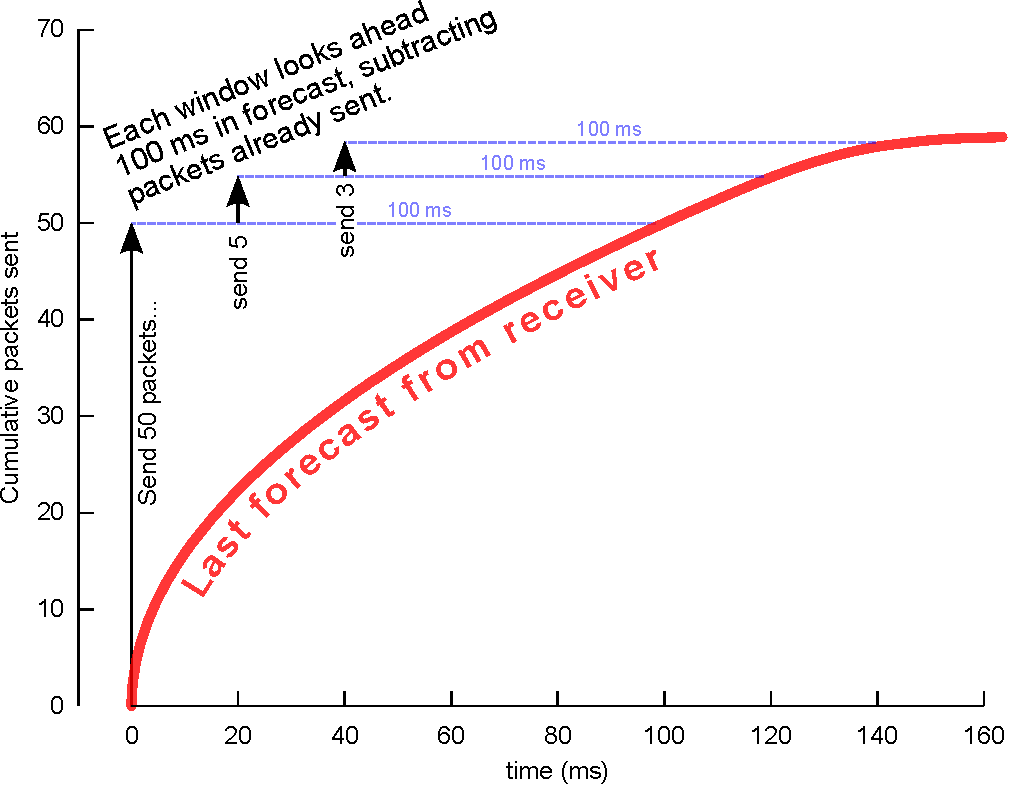
\includegraphics[width=\columnwidth]{forecast.pdf}

\label{f:forecast}

\end{figure}

The Sprout sender uses the most recent forecast it has obtained from the
receiver to calculate a window size---the number of bytes it may
safely transmit, while ensuring that every packet has 95\% probability
of clearing the queue within 100~ms (a conventional standard for
interactivity). Upon receipt of the forecast, the sender timestamps it and
estimates the current queue occupancy, based on the difference between
the number of bytes it has sent so far and the ``received-or-lost''
sequence number in the forecast.

The sender maintains its estimate of queue occupancy going
forward. For every byte it sends, it increments the estimate. Every
time it advances into a new tick of the 8-tick forecast, it decrements
the estimate by the amount of the forecast, bounding the estimate
below at zero packets.

To calculate a window size that is safe for the application to send,
Sprout looks ahead five ticks (100~ms) into the forecast's future, and
counts the number of bytes expected to be drained from the queue over
that time. Then it subtracts the current queue occupancy
estimate. Anything left over is ``safe to send''---bytes that we
expect to be cleared from the queue within 100~ms, even taking into
account the queue's current contents. This evolving window size
governs how much the application may transmit. Figure~\ref{f:forecast}
illustrates this process schematically.

As time passes, the sender may look ahead further and further into the
forecast (until it reaches 160~ms), even without receiving an update
from the receiver. In this manner, Sprout combines elements of pacing
with window-based flow control.

%\input{alf}
\section{Experimental testbed}
\label{s:impl}
\label{ss:platform}
We use trace-driven emulation to evaluate Sprout and compare it with
other applications and protocols under reproducible network
conditions. Our goal is to capture the variability of cellular
networks in our experiments and to evaluate each scheme under the same
set of time-varying conditions.

\subsection{Saturator} Our strategy is to characterize the behavior
of a cellular network by saturating its uplink and downlink at the
same time with MTU-sized packets, so that neither queue goes empty. We
record the times that packets actually cross the link, and we treat
these as the ground truth representing all the times that packets
\emph{could} cross the link as long as a sender maintains a backlogged
queue.

\label{ss:saturator}

Because even TCP does not reliably keep highly variable links
saturated, we developed our own tool. The Saturator runs on a laptop
tethered to a cell phone (which can be used while in a car) and on a
server that has a good, low-delay ($<$ 20~ms) Internet path to the
cellular carrier.

The sender keeps a window of $N$ packets in flight to the receiver,
and adjusts $N$ in order to keep the observed RTT greater than 750~ms
(but less than 3000~ms). The theory of operation is that if packets
are seeing more than 750~ms of queueing delay, the link is not
starving for offered load. (We do not exceed 3000~ms of delay because
the cellular network may start throttling or dropping packets.)

\begin{figure}
  \caption{Block diagram of Cellsim}
\hspace{\baselineskip}

\noindent \def\svgwidth{\columnwidth}\input{emu.pdf_tex}

\label{f:cellsim}

\end{figure}

There is a challenge in running this system in two directions at once
(uplink and downlink), because if both links are backlogged by
multiple seconds, feedback arrives too slowly to reliably keep both
links saturated. Thus, the Saturator laptop is actually connected to
\emph{two} cell phones. One acts as the ``device under test,'' and its
uplink and downlink are saturated.  The second cell phone is used only
for short feedback packets and is otherwise kept unloaded. In our
experiments, the ``feedback phone'' was on Verizon's LTE network,
which provided satisfactory performance: generally about 20~ms delay
back to the server at MIT.

We collected data from four commercial cellular networks: Verizon
Wireless's LTE and 3G (1xEV-DO / eHRPD) services, AT\&T's LTE service,
and T-Mobile's 3G (UMTS) service.\footnote{We also attempted a
  measurement on Sprint's 3G (1xEV-DO) service, but the results
  contained several lengthy outages and were not further analyzed.} We
drove around the greater Boston area at rush hour and in the evening
while recording the timings of packet arrivals from each network,
gathering about 17 minutes of data from each. Because the traces were
collected at different times and places, the measurements cannot be
used to compare different commercial services head-to-head.

The Verizon LTE and 1xEV-DO (3G) traces
were collected with a Samsung Galaxy Nexus smartphone running Android 4.0. The AT\&T
trace used a Samsung Galaxy S3 smartphone running Android 4.0, and the
T-Mobile trace used a Samsung Nexus S smartphone running Android 4.1.

\subsection{Cellsim}

We then replayed the traces in a network emulator, which we call
Cellsim (Figure~\ref{f:cellsim}). It runs on a PC and takes in packets
on two Ethernet interfaces, delays them for a configurable amount of
time (the propagation delay), and adds them to the tail of a
queue. Cellsim releases packets from the head of the queue to the
other network interface according to the same trace that was
previously recorded by Saturator. If a scheduled packet delivery
occurs while the queue is empty, nothing happens and the opportunity
to deliver a packet is wasted.\footnote{This accounting is done on a
  per-byte basis. If the queue contains 15 100-byte packets, they will
  all be released when the trace records delivery of a single
  1500-byte (MTU-sized) packet.}

Empirically, we measure a one-way delay of about 20~ms in each
direction on our cellular links (by sending a single packet in one
direction on the uplink or downlink back to a desktop with good
Internet service). All our experiments are done with this
propagation delay, or in other words a 40~ms minimum RTT.

Cellsim serves as a transparent Ethernet bridge for a Mac or PC under
test. A second computer (which runs the other end of the connection)
is connected directly to the Internet. Cellsim and the second computer
receive their Internet service from the same gigabit Ethernet switch.

We tested the latest (September 2012) real-time implementations of all
the applications and protocols (Skype, Facetime, etc.) running on
separate late-model Macs or PCs (Figure~\ref{f:software}).

\begin{figure}
  \caption{Software versions tested}
\hspace{\baselineskip}

\begin{centering}

\label{f:software}

%\scriptsize
\noindent \begin{tabular}{|l|l|l|l|}
\hline
Program & Version & OS & Endpoints \\
\hline
\hline
Skype & 5.10.0.116 & Windows 7 & Core i7 PC \\
Hangout & as of 9/2012 & Windows 7 & Core i7 PC \\
Facetime & 2.0 (1070) & OS X 10.8.1 & MB Pro (2.3 GHz i7),\\
& & & MB Air (1.8 GHz i5) \\
TCP Cubic & in Linux 3.2.0 & & Core i7 PC \\
TCP Vegas & in Linux 3.2.0 & & Core i7 PC \\
LEDBAT & in $\mu$TP & Linux 3.2.0 & Core i7 PC \\
Compound TCP & in Windows 7 & & Core i7 PC \\
\hline
\end{tabular}

\end{centering}
\end{figure}

We also added stochastic packet losses to Cellsim to study Sprout's
loss resilience. Here, Cellsim drops packets from the tail of the
queue according to a specified random drop rate.  This approach
emulates, in a coarse manner, cellular networks that do not have deep
packet buffers (e.g., Clearwire, as reported
in~\cite{Mahajan12}). Cellsim also includes an optional implementation
of CoDel, based on the pseudocode in ~\cite{CoDel}.

\subsection{SproutTunnel}

We implemented a UDP tunnel that uses Sprout to carry arbitrary
traffic (e.g.~TCP, videoconferencing protocols) across a cellular link
between a mobile user and a well-connected host, which acts as a relay
for the user's Internet traffic. SproutTunnel provides each flow with
the abstraction of a low-delay connection, without modifying carrier
equipment. It does this by separating each flow into its own queue,
and filling up the Sprout window in round-robin fashion among the
flows that have pending data.

The total queue length of all flows is limited to the receiver's most
recent estimate of the number of packets that can be delivered over
the life of the forecast. When the queue lengths exceed this value,
the tunnel endpoints drop packets from the head of the longest
queue. This algorithm serves as a dynamic traffic-shaping or
active-queue-management scheme that adjusts the amount of buffering to
the predicted channel conditions.

\section{Evaluation}
\label{sprout:eval}

This section presents our experimental results obtained using the
testbed described
in \S\ref{ss:platform}. We start by motivating and defining the two
main metrics: throughput and self-inflicted delay. We then compare
Sprout with Skype, Facetime, and Hangout, focusing on how the
different rate control algorithms used by these systems affect the
metrics of interest. We compare against the delay-triggered congestion
control algorithms TCP Vegas and LEDBAT, as well as the
default TCP in Linux, Cubic, which does not use delay as a
congestion signal, and Compound TCP, the default in some
versions of Windows.

We also evaluate a simplified version of Sprout, called Sprout-EWMA,
that eliminates the cautious packet-delivery forecast in favor of an
exponentially-weighted moving average of observed throughput. We
compare both versions of Sprout with a queue-management technique that
must be deployed on network infrastructure. We also measure Sprout's
performance in the presence of packet loss.

Finally, we evaluate the performance of competing flows (TCP Cubic
and Skype) running over the Verizon LTE downlink, with and without
SproutTunnel.

The implementation of Sprout (including the tuning parameters $\sigma
= 200$ and $\lambda_z = 1$) was frozen before collecting the network
traces, and has not been tweaked.
% However, SproutTunnel and its AQM
%scheme were designed and evaluated after the network traces were
%collected and the rest of the evaluation had been conducted.

\subsection{Metrics}

We are interested in performance metrics appropriate for a real-time
interactive application. In our evaluation, we report the
\emph{average throughput} achieved and the 95th-percentile
\emph{self-inflicted delay} incurred by each protocol, based on
measurement of packet entry and exit from the Cellsim.

The \emph{throughput} is the total number of bits received by an
application, divided by the duration of the experiment. We use this as
a measure of bulk transfer rate.

The {\em self-inflicted delay} is a lower bound on the end-to-end
delay that must be experienced between a sender and receiver, given
observed network behavior. We define it as follows: At any point in
time, we find the most recently sent packet to have arrived at the
receiver. The amount of time since this packet was sent is a lower
bound on the instantaneous delay that must exist between the sender's
input and receiver's output in order to avoid a gap in playback or
other glitch at this moment. We calculate this instantaneous delay for
each moment in time. The 95th percentile of this function (taken over the
entire trace) is the amount of delay that must exist between the input
and output so that the receiver can recover 95\%~of the input signal
by the time of playback. We refer to this as ``95\%~end-to-end
delay.''

For a given trace, there is a lower limit on the 95\%~end-to-end delay
that can be achieved even by an omniscient protocol: one that sends
packets timed to arrive exactly when the network is ready to dequeue
and transmit a packet. This ``omniscient'' protocol will achieve
100\%~of the available throughput of the link and its packets will
never sit in a queue. Even so, the ``omniscient'' protocol will have
fluctuations in its 95\%~end-to-end delay, because the link may have
delivery outages. If the link does not deliver any packets for 5
seconds, there must be at least 5 seconds of end-to-end delay to avoid
a glitch, no matter how smart the protocol is.\footnote{If packets are
  not reordered by the network, the definition becomes simpler. At
  each instant that a packet arrives, the end-to-end delay is equal to
  the delay experienced by that packet. Starting from this value, the
  end-to-end delay increases linearly at a rate of 1 s/s, until the
  next packet arrives. The 95th percentile of this function is the
  95\%~end-to-end delay.}

The difference between the 95\%~end-to-end delay measured for a
particular protocol and for an ``omniscient'' one is known as the
\emph{self-inflicted delay}. This is the appropriate figure to assess
a real-time interactive protocol's ability to compromise between
throughput and the delay experienced by users.

To reduce startup effects when measuring the average throughput and
self-inflicted delay from an application, we skip the first minute of
each application's run.

\subsection{Comparative performance}

\begin{figure*}
\caption{Throughput and delay of each protocol over the traced
  cellular links. Better results are up and to the right.}

\vspace{\baselineskip}
\begin{centering}
\noindent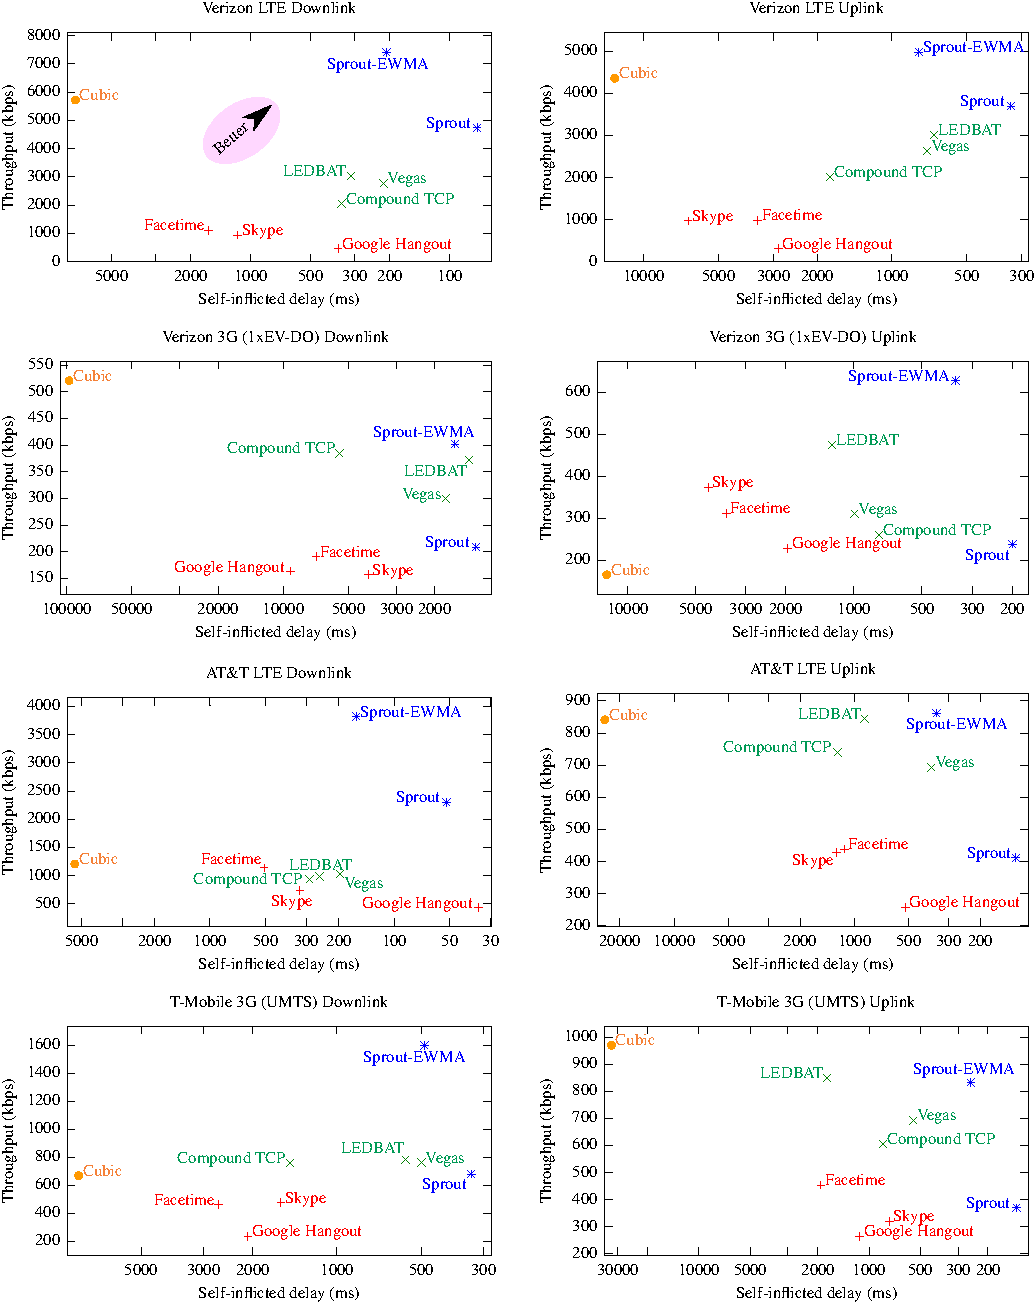
\includegraphics[width=\textwidth]{graphs-out.pdf}

\end{centering}

\label{f:allgraphs}

\end{figure*}

Figure~\ref{f:allgraphs} presents the results of our trace-driven
experiments for each transport protocol. The figure shows eight
charts, one for each of the four measured networks, and for each data
transfer direction (downlink and uplink). On each chart, we plot one
point per application or protocol, corresponding to its measured
throughput and self-inflicted delay combination. For interactive
applications, high throughput and low delay (up and to the right) are
the desirable properties. The table in the introduction shows the
average of these results, taken over all the measured networks and
directions, in terms of the average relative throughput gain and delay
reduction achieved by Sprout.

We found that Sprout had the lowest, or close to the lowest, delay
across each of the eight links. On average delay, Sprout was lower
than every other protocol. On average throughput, Sprout outperformed
every other protocol except for Sprout-EWMA and TCP Cubic.

We also observe that Skype, Facetime, and Google Hangout all have
lower throughput and higher delay than the TCP congestion-control
algorithms. We believe this is because they do not react to rate
increases and decreases quickly enough, perhaps because they are
unable to change the encoding rapidly, or unwilling for perceptual
reasons.\footnote{We found that the complexity of the video signal did
  not seem to affect these programs' transmitted throughputs. On fast
  network paths, Skype uses up to 5 Mbps even when the image is
  static.} By continuing to send when the network has dramatically
slowed, these programs induce high delays that destroy interactivity.

\subsection{Benefits of forecasting}

Sprout differs from the other approaches in two significant ways:
first, it uses the packet arrival process at the receiver as the
``signal'' for its control algorithm (as opposed to one-way delays as
in LEDBAT or packet losses or round-trip delays in other protocols),
and second, it models the arrivals as a flicker-noise process to
perform Bayesian inference on the underlying rate. A natural question
that arises is what the benefits of Sprout's forecasting are. To
answer this question, we developed a simple variant of Sprout, which
we call {\em Sprout-EWMA}. Sprout-EWMA uses the packet arrival times,
but rather than do any inference with that data, simply passes them
through an exponentially-weighted moving average (EWMA) to produce an
evolving smoothed rate estimate. Instead of a cautious
``95\%-certain'' forecast, Sprout-EWMA simply predicts that the link will
continue at that speed for the next eight ticks. The rest of the
protocol is the same as Sprout.

The Sprout-EWMA results in the eight charts in Figure~\ref{f:allgraphs}
show how this protocol performs. First, it out-performs all the
methods in throughput, including recent TCPs such as Compound TCP and
Cubic. These results also highlight the role of cautious forecasting:
the self-inflicted delay is significantly lower for Sprout compared
with Sprout-EWMA. TCP Vegas also achieves lower delay on average than
Sprout-EWMA. The reason is that an EWMA is a low-pass filter, which
does not immediately respond to sudden rate reductions or outages (the
tails seen in Figure~\ref{f:vzinter}). Though these occur with low
probability, when they do occur, queues build up and take a
significant amount of time to dissipate.  Sprout's forecasts provide a
conservative trade-off between throughput and delay: keeping delays
low, but missing legitimate opportunities to send
packets, preferring to avoid the risk of filling up queues. Because
the resulting throughput is relatively high, we believe it is a good
choice for interactive applications. An application that is interested
only in high throughput with less of an emphasis on low delay may prefer
Sprout-EWMA.

\subsection{Comparison with in-network changes}

We compared Sprout's end-to-end inference approach against an
in-network deployment of active queue management. We added the CoDel
AQM algorithm~\cite{CoDel} to Cellsim's uplink and downlink queue, to
simulate what would happen if a cellular carrier installed this
algorithm inside its base stations and in the baseband modems or
radio-interface drivers on a cellular phone.

The average results are shown in Figure~\ref{f:codelchart}. Averaged
across the eight cellular links, CoDel dramatically reduces the delay
incurred by Cubic, at little cost to throughput.

Although it is purely end-to-end, Sprout's delays are even lower than
Cubic-over-CoDel. However, this comes at a cost to
throughput. (Numerical results are given in Figure~\ref{f:sproutvsaqm}.)
Sprout-EWMA achieves within 6\% of the same delay as Cubic-over-CoDel,
with 30\% more throughput.

Rather than embed a single throughput-delay tradeoff into the network
(e.g.~by installing CoDel on carrier infrastructure), we believe it
makes architectural sense to provide endpoints and applications with
such control when possible. Users should be able to decide which
throughput-delay compromise they prefer. In this setting, it appears
achievable to match or even exceed CoDel's performance without
modifying gateways.

\begin{figure}
\caption{Average utilization and delay of each scheme. Utilization is
  the average fraction of the cellular link's maximum capacity that
  the scheme achieved.}

\vspace{\baselineskip}

%\footnotesize
\def\svgwidth{\columnwidth}\input{codelcomp.pdf_tex}

\label{f:codelchart}

\end{figure}

\begin{figure}
\caption{Lowering the forecast's confidence parameter allows greater
  throughput at the cost of more delay. Results on the T-Mobile 3G (UMTS)
  uplink:}

\vspace{\baselineskip}

%\footnotesize
\def\svgwidth{\columnwidth}\input{varySprout2.pdf_tex}

\label{f:varysprout}

\end{figure}

\subsection{Effect of confidence parameter}

The Sprout receiver makes forecasts of a lower bound on how many
packets will be delivered with at least 95\% probability. We explored
the effect of lowering this confidence parameter to express a greater
willingness that packets be queued for longer than the sender's 100~ms
tolerance.

Results on one network path are shown in
Figure~\ref{f:varysprout}. The different confidence parameters trace
out a curve of achievable throughput-delay tradeoffs. As expected,
decreasing the amount of caution in the forecast allows the sender to
achieve greater throughput, but at the cost of more delay.
Interestingly, although Sprout achieves higher throughput and lower
delay than Sprout-EWMA by varying the confidence parameter, it never
achieves both at the same time. Why this is---and whether Sprout's
stochastic model can be further improved to beat Sprout-EWMA
simultaneously on both metrics---will need to be the subject of
further study.

\subsection{Loss resilience}
\label{ss:loss}

The cellular networks we experimented with all exhibited low packet
loss rates, but that will not be true in general. To investigate the
loss resilience of Sprout, we used the traces collected from one
network (Verizon LTE) and simulated Bernoulli packet losses
(tail drop) with two different packet loss probabilities, 5\% and 10\%
(in each direction). The results are shown in the table below:
\begin{center}
\small
\begin{tabular}{|l|c|c|}
\hline
 Protocol & Throughput (kbps) & Delay (ms) \\
\hline
\hline
\multicolumn{3}{|c|}{\bf Downlink} \\
\hline
Sprout & 4741 & 73 \\
Sprout-5\% & 3971 & 60 \\
Sprout-10\% & 2768 & 58\\
\hline
\multicolumn{3}{|c|}{\bf Uplink} \\
\hline
Sprout & 3703 & 332 \\
Sprout-5\% & 2598 & 378 \\
Sprout-10\% & 1163 & 314\\
\hline
\end{tabular}
\end{center}

As expected, the throughput does diminish in the face of packet loss,
but Sprout continues to provide good throughput even at high loss
rates. (TCP, which interprets loss as a congestion signal, generally
suffers unacceptable slowdowns in the face of 10\% each-way packet
loss.) These results demonstrate that Sprout is relatively resilient to
packet loss.

\subsection{Sprout as a tunnel for competing traffic}

We tested whether SproutTunnel, used as a tunnel over the
cellular link to a well-connected relay, can successfully isolate
bulk-transfer downloads from interactive applications.

We ran two flows: a TCP Cubic bulk transfer (download only) and a
two-way Skype videoconference, using the Linux version of Skype.

We compared the situation of these two flows running directly over the
emulated Verizon LTE link, versus running them through SproutTunnel
over the same link. The experiments lasted about ten minutes
each.\footnote{In each run, Skype ended the video portion of the call
  once and was restarted manually.}

\begin{center}
{
\small
\noindent \begin{tabular}{|l|l|l|l|}
\hline
& Direct & via Sprout & Change \\
\hline
\hline
Cubic throughput & 8336 kbps & 3776 kbps & \cellcolor{red!20}$-55\%$ \\
Skype throughput & 78 kbps & 490 kbps & \cellcolor{blue!20}$+528\%$ \\
Skype 95\% delay & 6.0~s & 0.17~s & \cellcolor{blue!20}$-97\%$ \\
\hline
\end{tabular}
}
\end{center}

The results suggest that interactive applications can be greatly aided
by running their traffic---and any concurrent bulk transfers---through
Sprout. Without Sprout to mediate, Cubic squeezes out Skype and builds
up huge delays. However, Sprout's conservatism about delay
substantially reduces Cubic's throughput.

\vspace{\baselineskip}

%\end{center}

% \subsubsection{Skype}
% \subsubsection{Facetime}
% \subsubsection{Hangouts}

% \subsection{Comparisons to congestion control algorithms}

% \subsubsection{TCP CUBIC}

% \subsubsection{Compound TCP}

% \subsubsection{TCP Vegas}

% \subsubsection{TCP CUBIC + Codel}

% \subsubsection{LEDBAT}

\section{Related work}
\label{sprout:related}

\paragraph{End-to-end algorithms.}
%Although a large number of congestion control algorithms have been
%developed over the past three decades, 

Traditional congestion-control algorithms generally do not
simultaneously achieve high utilization and low delay over paths with
high rate variations.
%They also often introduce long and variable
%delays.
Early TCP variants such as Tahoe and Reno~\cite{Jacobson88} do not
explicitly adapt to delay (other than from ACK clocking), and require
an appropriate buffer size for good performance. TCP
Vegas~\cite{Brakmo94}, FAST~\cite{FAST}, and Compound TCP~\cite{CTCP}
incorporate round-trip delay explicitly, but the adaptation is
reactive and does not directly involve the receiver's observed rate.

LEDBAT~\cite{ledbat} (and TCP Nice~\cite{tcpnice}) share our goals of
high throughput without introducing long delays, but LEDBAT does not
perform as well as Sprout. We believe this is because of its choice of
congestion signal (one-way delay) and the absence of forecasting.
Some recent work proposes TCP receiver modifications to combat
bufferbloat in 3G/4G wireless networks~\cite{tcpbufferbloat}.
%We note
%that it is not enough to reactively throttle the receiver window when
%delays rise, because one needs mechanisms to predict rate increases
%and outages as well.
Schemes such as ``TCP-friendly'' equation-based
rate control~\cite{ebcc} and binomial congestion
control~\cite{binomial} exhibit slower transmission rate variations
than TCP, and in principle could introduce lower delay, but perform
poorly in the face of sudden rate changes~\cite{slowcc-dynamic}.

Google has proposed a congestion-control scheme~\cite{WebRTCdraft} for
the WebRTC system that uses an arrival-time filter at the receiver,
along with other congestion signals, to decide whether a real-time
flow should increase, decrease, or hold its current bit rate. We plan
to investigate this system and assess it on the same metrics as the
other schemes in our evaluation.

%In contrast to all these schemes, Sprout uses the observed
%distribution of packet interarrivals at the receiver as a signal,
%and incorporates stochastic predictions to forecast future rates that
%balance bit rate and delay. Rate forecasts allow Sprout to react on
%time scales faster than the round-trip time of the connection, which
%is unusual behavior for an end-to-end scheme. 
%Sprout's forecasts bear
%some similarity with the approach presented in a Hotnets position
%paper~\cite{WB11} (both deal with network uncertainty), but the
%problems tackled and the methods proposed in that paper are completely
%different.
\vspace{\baselineskip}
\noindent \textbf{Active queue management.} Active queue management schemes such as RED~\cite{Floyd93} and its
variants, BLUE~\cite{BLUE}, AVQ~\cite{AVQ}, etc., drop or mark packets
using local indications of upcoming congestion at a bottleneck queue,
with the idea that endpoints react to these signals before queues
grow significantly. Over the past several years, it has proven
difficult to automatically configure the parameters used in these
algorithms. To alleviate this shortcoming, CoDel~\cite{CoDel} changes
the signal of congestion from queue length to the delay experienced by
packets in a queue, with a view toward controlling that delay,
especially in networks with deep queues
(``bufferbloat''~\cite{bufferbloat}).

Our results show that Sprout largely holds its own with CoDel over
challenging wireless conditions without requiring any gateway
modifications. It is important to note that network paths in practice
have several places where queues may build up (in LTE infrastructure, in baseband modems, in IP-layer
queues, near the USB interface in tethering mode, etc.), so one may
need to deploy CoDel at all these locations, which could be
difficult. However, in networks where there is a lower degree of
isolation between queues than the cellular networks we study, CoDel
may be the right approach to controlling delay while providing good
throughput, but it is a ``one-size-fits-all'' method that assumes
that a single throughput-delay tradeoff is right for all traffic. 
%

% Sprout is end-to-end; it does not require any AQM at the bottleneck
% gateways, and might work well if all the sources in the network used
% it. That, however, is a difficult test to conduct in practice, so the
% immediately deployable ``use case'' is in cellular wireless networks
% where per-user queueing and (weighted and channel-dependent)
% round-robin scheduling is the norm. Per-user queues have traditionally
% been viewed as ``non-scalable'' in the folklore of Internet
% architecture, but cellular networks (for all their other shortcomings)
% demonstrate that such isolation is both practical and useful (e.g.,
% for accounting, billing, providing loose rate guarantees tied to
% subscriptions, etc.).  For wired networks with fair queueing gateways,
% a good congestion control solution is the packet-pair
% scheme~\cite{packetpair}, which relies on transmitting pairs (or
% bunches) of back-to-back packets to determine transmission rates. This
% method works well when the link rate is constant, but when link rates
% vary quickly, packet-pair methods are unlikely to work well.

%\paragraph{Adaptive applications.}
%In terms of application-layer adaptation, Alfalfa's new interface to
%video codec libraries enables finer-grained adaptation compared with
%other systems. Our use is an example of Application-Level Framing
%(ALF)~\cite{alf}, but unlike previous ALF-inspired applications, the
%adaptation is at a finer grain. Alfalfa does not just pick a suitable
%application data unit (ADU) from pre-determined choices, but instead
%constructs data frames dynamically using knowledge of previous
%receptions as well as the forecasted network conditions.  The ALF
%principle has been used in a variety of media delivery protocols and
%architectural proposals, including RTP~\cite{RTP}, MBone
%applications~\cite{Mbone}, the Congestion Manager API~\cite{cm},
%etc. Much of the previous work on ALF-inspired protocols has focused
%on handling packet losses~\cite{audio-perkins,cmvideo}, whereas in
%cellular networks the main problem is coping with rapid rate variations.

\section{Limitations and Future Work}

Although our results are encouraging, there are several limitations to
our work. First, as noted in \S\ref{s:problem} and \S\ref{s:sprout},
an end-to-end system like Sprout cannot control delays when the
bottleneck link includes competing traffic that shares the same
queue. If a device uses traditional TCP outside of Sprout, the
incurred queueing delay---seen by Sprout and every flow---will be
substantial.

Sprout is not a traditional congestion-control protocol, in that it is
designed to adapt to varying link conditions, not varying cross
traffic. In a cellular link where users have their own queues on the
base station, interactive performance will likely be best when the
user runs bulk and interactive traffic \emph{inside} Sprout
(e.g.~using SproutTunnel), not alongside Sprout. We have not evaluated
the performance of multiple Sprouts sharing a queue.
% We leave to
%future work a better understanding of the {\em need} for active queue
%management to achieve good throughput-delay trade-offs with multiple
%independent contending flows, speculating here that a purely
%end-to-end approach may in fact work.

The accuracy of Sprout's forecasts depends on whether the application
is providing offered load sufficient to saturate the link. For
applications that switch intermittently on and off, or don't desire
high throughput, the transient behavior of Sprout's forecasts
(e.g.~ramp-up time) becomes more important. We did not evaluate any
non-saturating applications in this paper or attempt to measure or optimize
Sprout's startup time from idle.

Finally, we have tested Sprout only in trace-based emulation of eight
cellular links recorded in the Boston area in 2012. Although Sprout's
model was frozen before data were collected and was not ``tuned'' in
response to any particular network, we cannot know how generalizable
Sprout's algorithm is without more real-world testing.

In future work, we are eager to explore different stochastic network
models, including ones trained on empirical variations in cellular
link speed, to see whether it is possible to perform much better than
Sprout if a protocol has more accurate forecasts. We think it will be
worthwhile to collect enough traces to compile a standardized
benchmark of cellular link behavior, over which one could evaluate any
new transport protocol.

\section{Conclusion}
\label{s:comcl}

This paper presented Sprout, a transport protocol for real-time
interactive applications over Internet paths that traverse cellular
wireless networks. Sprout improves on the performance of current
approaches by modeling varying networks explicitly. Sprout has two
interesting ideas: the use of packet arrival times as a congestion
signal, and the use of probabilistic inference to make a cautious
forecast of packet deliveries, which the sender uses to pace its
transmissions. Our experiments show that forecasting is important to
controlling delay, providing an end-to-end rate control algorithm that
can react at time scales shorter than a round-trip time.

Our experiments conducted on traces from four commercial cellular
networks show many-fold reductions in delay, and increases in
throughput, over Skype, Facetime, and Hangout, as well as over Cubic,
Compound TCP, Vegas, and LEDBAT. Although Sprout is an end-to-end
scheme, in this setting it matched or exceeded the performance of
Cubic-over-CoDel, which requires modifications to network
infrastructure to be deployed.

\section{Acknowledgments}
\label{s:acks}

We thank Shuo Deng, Jonathan Perry, Katrina LaCurts, Andrew McGregor,
Tim Shepard, Dave T\"{a}ht, Michael Welzl, Hannes Tschofenig, and the
anonymous reviewers for helpful discussion and feedback. This work was
supported in part by NSF grant 1040072. KW was supported by the Claude
E.~Shannon Research Assistantship. We thank the members of the MIT
Center for Wireless Networks and Mobile Computing, including
Amazon.com, Cisco, Google, Intel, Mediatek, Microsoft, ST
Microelectronics, and Telefonica, for their support.


\chapter{TCP ex Machina: Computer-Generated Congestion Control}
\label{chap:remy}

\begin{abstract}

  This paper describes a new approach to end-to-end congestion control
  on a multi-user network. Rather than manually formulate each
  endpoint's reaction to congestion signals, as in traditional
  protocols, we developed a program called Remy that generates
  congestion-control algorithms to run at the endpoints.

  In this approach, the protocol designer specifies their prior
  knowledge or assumptions about the network and an objective that the
  algorithm will try to achieve, e.g., high throughput and low
  queueing delay.  Remy then produces a distributed algorithm---the
  control rules for the independent endpoints---that tries to achieve
  this objective.

% Traditionally, congestion-control protocols
%  were developed by specifying the algorithm that endpoints run, so as
%  to achieve good performance and prevent congestion collapse.
%  We reverse this tradition. Instead of hand-crafting rules for
%  endpoint behavior, 
%In this approach, we specify an uncertain model of network scenarios
%and a utility function of throughput and delay. Remy then produces a
%distributed algorithm---that is, the control rules for the
%endpoints---that attempts to maximize the total utility.  Remy's
%output depends on the model of the network and workload, so it can
%change with time as network scenarios and workloads evolve.
%
% A computer
 % program called Remy then designs a congestion-control algorithm from
 % first principles in response to these inputs.
%The algorithm can be used by a TCP
%  sender, without changes to the receiver.

  In simulations with ns-2, Remy-generated algorithms
  outperformed human-designed end-to-end techniques, including TCP
  Cubic, Compound, and Vegas. In many cases, Remy's algorithms also
  outperformed methods that require intrusive in-network changes,
  including XCP and Cubic-over-sfqCoDel (stochastic fair queueing with
  CoDel for active queue management).

  Remy can generate algorithms both for networks where some parameters
  are known tightly \textit{a priori}, e.g.~datacenters, and for
  networks where prior knowledge is less precise, such as cellular
  networks. We characterize the sensitivity of the resulting
  performance to the specificity of the prior knowledge, and the
  consequences when real-world conditions contradict the assumptions
  supplied at design-time.

%\category{C.2.1}{Computer-Communication Networks}{Network Architecture
%  and Design --- Network communications}

%\keywords{congestion control, computer-generated algorithms}

%\terms{Design, Performance}

\end{abstract}

%\section{Introduction}
\label{remy:intro}

Sprout (Chapter~\ref{chap:sprout}) addressed a particular problem in
congestion control: the compromise between throughput and delay on a
cellular network, where the user has his or her own queue at the
bottleneck but does not know the capacity of the link.

The classical problem of distributed resource allocation on the
Internet, however, is more challenging than this. Algorithms like TCP
NewReno~\cite{newreno} and Cubic~\cite{cubic} are designed for the
problem of \emph{multi-agent} congestion control. In general, multiple
independent users may contend for the same bottleneck---without
knowing for certain how many other users they are contending with.

Is it possible, then, for a computer to design an algorithm from first
principles and ``discover'' the right rules for congestion control? We
found that computers can design schemes that in some cases surpass the
best human-designed methods to date, when supplied with the
appropriate criteria by which to judge a congestion-control
algorithm. We attempt to probe the limits of these machine-generated
protocols, and discuss how this style of transport-layer protocol
design can give more freedom to network architects and link-layer
designers.

\begin{figure}
\vspace{\baselineskip}
\begin{centering}
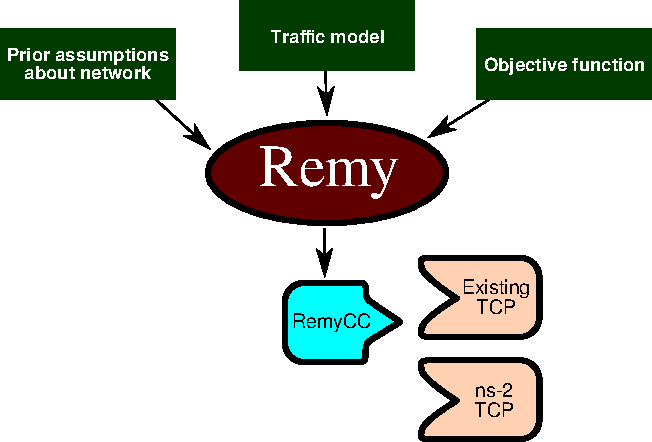
\includegraphics[width=0.75 \columnwidth]{remy.pdf}
\caption{Remy designs congestion-control schemes automatically to
  achieve desired outcomes. The algorithms it produces may replace
the congestion-control module of a TCP implementation, and fit into
a network library or kernel module that implements congestion
control (DCCP, SCTP, the congestion manager, application-layer
transmission control libraries, ns-2 modules, etc.).}

\end{centering}

\end{figure}

Congestion control is a fundamental problem in multi-user computer
networks. Any proposed solution must answer the question: when should
an endpoint transmit each packet of data? An ideal scheme would
transmit a packet whenever capacity to carry the packet was available,
but because there are many concurrent senders and the network
experiences variable delays, this question isn't an easy one to
answer. On the Internet, the past thirty years have seen a number of
innovative and influential answers to this question, with solutions
embedded at the endpoints (mainly in TCP) aided occasionally by queue
management and scheduling algorithms in bottleneck routers that
provide signals to the endpoints.

This area has continued to draw research and engineering effort
because new link technologies and subnetworks have proliferated and
evolved. For example, the past few years have seen an increase in
wireless networks with variable bottleneck rates; datacenter networks
with high rates, short delays, and correlations in offered load; paths
with excessive buffering (now called ``bufferbloat''); cellular
wireless networks with highly variable, self-inflicted packet delays;
links with non-congestive stochastic loss; and networks with large
bandwidth-delay products. In these conditions, the classical
congestion-control methods embedded in TCP can perform poorly, as many
papers have shown (\S\ref{remy:related}).

%Although the control methods in TCP have evolved over the past several
%years (indeed, there is no longer just one TCP scheme in practice),
%they are generally rooted in an implicit assumption that the Internet
%exhibits the same behaviors that it did in the 1980s. Classical TCP
%uses only three congestion signals: packet losses (assumed to be
%caused by buffer losses), the smoothed round-trip time (RTT), and the
%delay jitter (assumed to be a lightly-tailed
%distribution)~\cite{Jacobson88}. Newer phenomena, such as stochastic
%packet loss or heavy-tailed jitter, are not easily accounted for.

Without the ability to adapt its congestion-control algorithms to new
scenarios, TCP's inflexibility constrains architectural
evolution~\cite{hotnets2011}. Subnetworks and link layers are
typically evaluated based on how well TCP performs over them.  This
scorecard can lead to perverse behavior, because TCP's network model
is limited. For example, because TCP assumes that packet losses are
due to congestion and reduces its transmission rate in response, some
subnetwork designers have worked hard to hide losses. This often
simply adds intolerably long packet delays. One may argue that such
designs are misguided, but the difficulties presented by
``too-reliable'' link layers have been a perennial challenge for 25
years~\cite{Clark88} and show no signs of abating. With the rise of
widespread cellular connectivity, these behaviors are increasingly
common and deeply embedded in deployed infrastructure.

The designers of a new subnetwork may well ask what they should do to
make TCP perform well. This question is surprisingly hard to answer,
because the so-called teleology of TCP is unknown: exactly what
objective does TCP congestion control optimize? TCP's dynamic
behavior, when competing flows enter and leave the network, remains
challenging to explain~\cite{slowcc}.  In practice, the need to ``make
TCP perform well'' is given as a number of loose guidelines, such as
IETF RFC 3819~\cite{rfc3819}, which contains dozens of pages of
qualitative best current practice. The challenging and subtle nature
of this area means that the potential of new subnetworks and network
architectures is often not realized.

\section{Design overview}

%How should we design network protocols that free subnetworks and links
%to evolve freely, ensuring that the endpoints will adapt properly
%\emph{no matter what} the lower layers do?  We believe that the best
%way to approach this question is to take the design of specific
%algorithmic mechanisms out of the hands of human designers (no matter
%how sophisticated!), and make the end-to-end algorithm be a function
%of the desired overall behavior.

%These actions should not
%depend on explicit signals about unusual network behaviors, e.g., if a
%new network were to reorder packets because of multi-path routing,
%endpoints should not have to be notified.

We start by explicitly stating an {\em objective} for congestion
control; for example, given an unknown number of users, we may
optimize some function of the per-user throughput and packet delay, or
a summary statistic such as average flow completion time. Then,
instead of writing down rules by hand for the endpoints to follow, we
start from the desired objective and work backwards in three steps:

%\item We specify a utility function that quantifies the
%  benefit to each user of the network. As in other work, this is
%  generally a concave function of average throughput, so that a fair
%  allocation is preferred. We then subtract a concave function of the
%  user's average delay, to penalize induced latency.

%We have developed an alternate approach for end-to-end resource
%management and transmission control. 

\begin{enumerate}

\item First, model the protocol's prior assumptions about the network;
  i.e., the ``design range'' of operation. This model
  may be different, and have different amounts of uncertainty, for a
  protocol that will be used exclusively within a data center,
  compared with one intended to be used over a wireless link or one
  for the broader Internet. A typical model specifies upper and lower
  limits on the bottleneck link speeds, non-queueing delays, queue
  sizes, and degrees of multiplexing.
%The model represents the
%  designer's prior knowledge about the networks that the protocol will
%  encounter.

\item Second, define a traffic model for the offered load given to
  endpoints. This may characterize typical Web traffic, video
  conferencing, batch processing, or some mixture of these. It may
  be synthetic or based on empirical measurements.

\item Third, use the modeled network scenarios and traffic to design a
  congestion-control algorithm that can later be executed on endpoints.

\end{enumerate}

I developed an optimization tool called Remy that takes these models
as input, and designs a congestion-control algorithm that tries to
maximize the total expected value of the objective function, measured
over the set of network and traffic models. The resulting
pre-calculated, optimized algorithm is then run on actual endpoints;
no further learning happens after the offline optimization. The
optimized algorithm is run as part of an existing TCP sender
implementation, or within any congestion-control module. No receiver
changes are necessary (as of now).

\section{Summary of results}

Running on an 80-core server at MIT, Remy generally takes between a
few hours to a few days of wall-clock time (up to a CPU-year) to
generate congestion-control algorithms offline that work on a wide
range of network conditions.

Our main results from several simulation experiments
with Remy are as follows:

\begin{enumerate}

\item For networks broadly consistent with the assumptions provided to
  Remy at design time, the machine-generated algorithms dramatically
  outperform existing methods, including TCP Cubic, Compound TCP, and
  TCP Vegas.

\item Comparing Remy's algorithms with schemes that require
  modifications to network gateways, including Cubic-over-sfqCoDel and
  XCP, Remy generally matched or surpassed these schemes, despite
  being entirely end-to-end.
\end{enumerate}

%\subsection*{Outline}

% We describe our model of the problem in \S~\ref{model}, and the design
% of Remy's optimizer in \S~\ref{design}. In \S~\ref{eval}, we describe
% the results of a series of ns-2 simulations that compared Remy's
% algorithms to the best human-designed congestion-control
% algorithms. We found that, for networks whose parameters fall within
% the range of those provided to Remy at optimization time, the
% resulting computer-generated algorithm conclusively outforms existing
% methods, including TCP Cubic and Vegas.

% We also compared Remy's algorithms with more intrusive schemes that
% require modifications to network gateways, including
% Cubic-over-sfqCoDel and XCP. Remy also outperformed or matched these
% schemes, despite being entirely end-to-end.

% A significant concern with any machine-learned method is its
% generalizability to situations not seen during training.\footnote{The
%   same risk of overfitting may arguably apply to human-designed
%   algorithms. For example, traditional congestion control was built on
%   the assumption that even when a gateway buffer is full enough that
%   it is dropping packets, the induced queueing delay is still
%   acceptable to other users. On contemporary network paths that do not
%   meet this constraint, including wireless links and ``bufferbloated''
%   home connections, TCP performs poorly. However, the problem of
%   overfitting is generally thought to be more acute with computer-designed
%   methods.} We attempt to characterize this phenomenon as it
% applies to Remy by measuring its performance as we vary network
% parameters to fall further and further outside the range seen during
% training.

On a simulated 15~Mbps fixed-rate link with eight senders contending and
an RTT of 150~ms, a computer-generated congestion-control algorithm
achieved the following improvements in median throughput and
reductions in median queueing delay over these existing protocols:

\label{sec:remyresults}

\begin{center}

\begin{tabular}{|l|c|c|}
\hline
Protocol & Median speedup & Median delay reduction \\
\hline
\hline
Compound & $2.1\times$ & $2.7\times$ \\
NewReno & $2.6\times$ & $2.2\times$ \\
Cubic & $1.7\times$ & $3.4\times$ \\
Vegas & $3.1\times$ & $1.2\times$ \\
\hline
Cubic/sfqCoDel & $1.4\times$ & $7.8\times$ \\
XCP & $1.4\times$ & $4.3\times$ \\
\hline
\end{tabular}

\end{center}

In a trace-driven simulation of the Verizon LTE downlink with four
senders contending, the \emph{same} computer-generated protocol achieved these
speedups and reductions in median queueing delay:

\begin{center}
\begin{tabular}{|l|c|c|}
\hline
Protocol & Median speedup & Median delay reduction \\
\hline
\hline
Compound & $1.3\times$ & $1.3\times$ \\
NewReno & $1.5\times$ & $1.2\times$ \\
Cubic & $1.2\times$ & $1.7\times$ \\
Vegas & $2.2\times$ & \cellcolor{red!20}$0.44\times$ \\
\hline
Cubic/sfqCoDel & $1.3\times$ & $1.3\times$ \\
XCP & $1.7\times$ & \cellcolor{red!20}$0.78\times$ \\
\hline
\end{tabular}

\end{center}

The source code for Remy, our ns-2 models, the algorithms that Remy
designed, and instructions for replicating the experiments and
reproducing the figures in this chapter are available from
\mbox{\url{http://mit.edu/remy}}.

\section{Related work}
\label{remy:related}

Starting with Ramakrishnan and Jain's DECBit scheme~\cite{decbit} and
Jacobson's TCP Tahoe (and Reno) algorithms~\cite{Jacobson88},
congestion control over heterogeneous packet-switched networks has
been an active area of research. End-to-end algorithms typically
compute a congestion window (or, in some cases, a transmission rate)
as well as the round-trip time (RTT) using the stream of
acknowledgments (ACKs) arriving from the receiver. In response to
congestion, inferred from packet loss or, in some cases, rising
delays, the sender reduces its window; conversely, when no congestion
is perceived, the sender increases its window.

There are many different ways to vary the window. Chiu and
Jain~\cite{chiujain} showed that among linear methods, additive
increase / multiplicative decrease (AIMD) converges to high
utilization and a fair allocation of throughputs, under some
simplifying assumptions (long-running connections with synchronized
and instantaneous feedback). Our work relaxes these assumptions to
handle flows that enter and leave the network, and users who care
about latency as well as throughput. Remy's algorithms are not
necessarily linear, and can use both a window and a rate pacer to
regulate transmissions.

In evaluating Remy, we compare its output---the computer-generated
algorithms---with several end-to-end schemes, including
NewReno~\cite{newreno}, Vegas~\cite{vegas}, Compound
TCP~\cite{compound}, Cubic~\cite{cubic}, and DCTCP for
datacenters~\cite{dctcp}. NewReno has the same congestion-control
strategy as Reno---slow start at the beginning, on a timeout, or after
an idle period of about one retransmission timeout (RTO), additive
increase every RTT when there is no congestion, and a one-half
reduction in the window on receiving three duplicate ACKs (signaling
packet loss). We compare against NewReno rather than Reno because
NewReno's loss recovery is better.

Brakmo and Peterson's Vegas is a delay-based algorithm, motivated by
the insight from Jain's CARD scheme~\cite{card} and Wang and Crowcroft's
DUAL scheme~\cite{dual} that increasing RTTs may be a congestion
signal.  Vegas computes a BaseRTT, defined as the RTT in the absence
of congestion, and usually estimated as the first RTT on the
connection before the windows grow. The expected throughput of the
connection is the ratio of the current window size and BaseRTT, if
there is no congestion; Vegas compares the {\em actual} sending rate,
and considers the difference, {\em diff}, between the expected and
actual rates.  Depending on this difference, Vegas either increases
the congestion window linearly ({\em diff} $< \alpha$), reduces it
linearly ({\em diff} $> \beta$), or leaves it unchanged.

Compound TCP~\cite{compound} combines ideas from Reno and Vegas: when
packet losses occur, it uses Reno's adaptation, while reacting to
delay variations using ideas from Vegas. Compound TCP is more
complicated than a straightforward hybrid of Reno and Vegas; for
example, the delay-based window adjustment uses a binomial
algorithm~\cite{binomial}. Compound TCP uses the delay-based window to
identify the absence of congestion rather than its onset, which is a
key difference from Vegas.

Rhee and Xu's Cubic algorithm is an improvement over their previous
work on BIC~\cite{bic}. Cubic's growth is independent of the RTT (like
H-TCP~\cite{htcp}), and depends only on the packet loss rate,
incrementing as a cubic function of ``real'' time. Cubic is known to
achieve high throughput and fairness independent of RTT, but it also
aggressively increases its window size, inflating queues and bloating
RTTs (see \S\ref{remy:eval}).

Other schemes developed in the literature include equation-based
congestion control~\cite{ebcc}, binomial control~\cite{binomial},
FastTCP~\cite{fasttcp}, HSTCP, and TCP Westwood~\cite{westwood}.

End-to-end control may be improved with explicit router participation,
as in Explicit Congestion Notification (ECN)~\cite{ecn},
VCP~\cite{vcp}, active queue management schemes like
RED~\cite{Floyd93}, BLUE~\cite{BLUE}, CHOKe~\cite{choke},
AVQ~\cite{AVQ}, and CoDel~\cite{CoDel} fair queueing, and explicit
methods such as XCP~\cite{xcp} and RCP~\cite{rcp}.  AQM schemes aim to
prevent persistent queues, and have largely focused on reacting to
growing queues by marking packets with ECN or dropping them even
before the queue is full. CoDel changes the model from reacting to
specific average queue lengths to reacting when the delays measured
over some duration are too long, suggesting a persistent
queue. Scheduling algorithms isolate flows or groups of flows from
each other, and provide weighted fairness between them.  In XCP and
RCP, routers place information in packet headers to help the senders
determine their window (or rate). One limitation of XCP is that it
needs to know the bandwidth of the outgoing link, which is difficult
to obtain accurately for a time-varying wireless channel.

In \S\ref{remy:eval}, we compare Remy's generated algorithm with XCP and
with end-to-end schemes running through a gateway with the CoDel AQM and
stochastic fair queueing (sfqCoDel).

TCP congestion control was not designed with an explicit optimization
goal in mind, but instead allows overall network behavior to emerge
from its rules. Kelly et al.~present an interpretation of various TCP
congestion-control variants in terms of the implicit goals they
attempt to optimize~\cite{Kelly98}.  This line of work has become
known as Network Utility Maximization (NUM); more recent work has
modeled stochastic NUM problems~\cite{stochasticnum}, in which flows
enter and leave the network. Remy may be viewed as combining the
desire for practical distributed endpoint algorithms with the explicit
utility-maximization ethos of stochastic NUM.

We note that TCP stacks have adapted in some respects to the changing
Internet; for example, increasing bandwidth-delay products have
produced efforts to increase the initial congestion
window~\cite{dukkipati2010argument,chu2012increasing}, including
recent proposals \cite{allman2010init,touch2012automating} for this
quantity to automatically increase on the timescale of months or
years. Remy represents an automated means by which TCP's entire
congestion-control algorithm, not just its initial window, could adapt
in response to empirical variations in underlying networks.



%Remy is a distributed POMDP-style method... Say something more here.

\section{Modeling the congestion-control problem}
\label{s:model}

We treat congestion control as a problem of distributed
decision-making under uncertainty. Each endpoint that has pending data
must decide for itself at every instant: send a packet, or don't
send a packet.

If all nodes knew in advance the network topology and capacity, and the
schedule of each node's present and future offered load, such
decisions could in principle be made perfectly, to achieve a desired
allocation of throughput on shared links.

In practice, however, endpoints receive observations that only hint at
this information. These include feedback from receivers concerning the
timing of packets that arrived and detection of packets that didn't, and
sometimes signals, such as ECN marks, from within the network itself.
Nodes then make sending decisions based on this partial information
about the network.

The Remy approach hinges on being able to evaluate quantitatively the
merit of any particular congestion control algorithm, and search for
the best algorithm for a given network model and objective function. I
describe here our models of the network and cross traffic, and how we
ultimately calculate a figure of merit for an arbitrary congestion
control algorithm.

\subsection{Expressing prior assumptions about the network}

From a node's perspective, we treat the network as having been drawn
from a stochastic generative process. We assume the network is
Markovian, meaning that it is described by some state (e.g.~the
packets in each queue) and its future evolution will depend only on
the current state.

We have parametrized networks on four axes: the speed of
bottleneck links, the number of bottlenecks, the propagation delay of the network paths, and the
degree of multiplexing, i.e., the number of senders contending for
each bottleneck link. We assume that senders have no control over the
paths taken by their packets to the receiver.

Depending on the range of networks over which the protocol is intended
to be used, a node may have more or less uncertainty about the
network's key parameters. For example, in a data center, the topology,
link speeds, and minimum round-trip times may be known in advance, but
the degree of multiplexing could vary over a large range. A virtual
private network between ``clouds'' may have more uncertainty about the
link speed. A wireless network path may experience less multiplexing,
but a large range of transmission rates and round-trip times.

We have observed only weak evidence for a tradeoff between generality
and performance; a protocol designed for a broad range of networks may
be beaten by a protocol that has been supplied with more specific and
accurate prior knowledge. Quantifying and characterizing these kind of
tradeoffs is the subject of Chapter~\ref{chap:learnability}.

\subsection{Traffic model}

Remy models the offered load as a stochastic process that switches
unicast flows between sender-receivers pairs on or off. In a simple
model, each endpoint has traffic independent of the other
endpoints. The sender is ``off'' for some number of seconds, drawn
from an exponential distribution. Then it switches on for some number
of bytes to be transmitted, drawn from an empirical distribution of
flow sizes or a closed-form distribution (e.g.~heavy-tailed
Pareto). While ``on,'' we assume that the sender will not stall until
it completes its transfer.

In traffic models characteristic of data center usage, the off-to-on
switches of contending flows may cluster near one another in time,
leading to incast. We also model the case where senders are ``on'' for
some amount of time (as opposed to bytes) and seek maximum throughput,
as in the case of videoconferences or similar real-time traffic.

\subsection{Objective function}

Resource-allocation theories of congestion control have traditionally
employed the alpha-fairness metric to evaluate allocations of
throughput on shared links~\cite{Srikant}. A flow that receives
steady-state throughput of $x$ is assigned a score of:

\begin{equation*}
U_\alpha(x) = \frac{x^{1-\alpha}}{1-\alpha}
\end{equation*}

As $\alpha \rightarrow 1$, in the limit $U_1(x)$ becomes $\log x$.

Because $U_\alpha(x)$ is concave for $\alpha > 0$ and monotonically
increasing, an allocation that maximizes the total score will prefer
to divide the throughput of a bottleneck link equally between
flows. When this is impossible, the parameter $\alpha$ sets the
tradeoff between fairness and efficiency. For example, $\alpha = 0$
assigns no value to fairness and simply measures total
throughput. $\alpha = 1$ is known as proportional fairness, because it
will cut one user's allocation in half as long as another user's can
be more than doubled. $\alpha = 2$ corresponds to minimum potential
delay fairness, where the score goes as the negative inverse of
throughput; this metric seeks to minimize the total time of
fixed-length file transfers. As $\alpha \rightarrow \infty$,
maximizing the total $U_\alpha(x)$ achieves max-min fairness, where
all that matters is the minimum resource allocations in bottom-up
order~\cite{Srikant}.

Because the overall score is simply a sum of monotonically increasing
functions of throughput, an algorithm that maximizes this total is
Pareto-efficient for any value of $\alpha$; i.e., the metric will
always prefer an allocation that helps one user and leaves all other
users the same or better. Tan et al.~\cite{Tan09} proved that, subject
to the requirement of Pareto-efficiency, alpha-fairness is \emph{the}
metric that places the greatest emphasis on fairness for a particular
$\alpha$.

Kelly et al.~\cite{Kelly98} and further analyses showed that TCP
approximately maximizes minimum potential delay fairness
asymptotically in steady state, if all losses are congestive and link
speeds are fixed.

We extend this model to cover dynamic traffic and network
conditions. Given a network trace, we calculate the average throughput
$x$ of each flow, defined as the total number of bytes received
divided by the time that the sender was ``on.'' We calculate the
average round-trip delay $y$ of the connection.

The flow's score is then 
\begin{equation*}
U_\alpha(\textrm{x}) - \delta \cdot U_\beta(\textrm{y}),
\label{eq:util}
\end{equation*}
where $\alpha$ and $\beta$ express the fairness-vs.-efficiency
tradeoffs in throughput and delay, respectively, and $\delta$
expresses the relative importance of delay vs.~throughput.% For the
%rest of this paper, we set $\alpha = \beta = 1$ and simply consider
%the sum of $\log(\textrm{throughput}) - \delta \cdot
%\log(\textrm{delay})$ for each flow.

%We also consider the metric of average flow completion time. This also
%expresses a throughput-vs.-delay tradeoff.

We emphasize that the purpose of the objective function is to supply a
quantitative goal from a protocol-design perspective. It need not
(indeed, does not) precisely represent users' ``true'' preferences or
utilities. In real usage, different users may have different
objectives; a videoconference may not benefit from more throughput, or
some packets may be more important than others. In
Chapter~\ref{chap:learnability}, we discuss the problem of how to
accommodate diverse objectives on the same network.

%In summary, this framework provides a unitary metric for evaluating
%the performance of any congestion-control endpoint algorithm (e.g.~TCP
%Cubic, Vegas, or Compound) on a given ensemble of network and traffic
%models. In the next section, we describe the design of the Remy
%program, which attempts to design a congestion-control algorithm to
%optimize this metric.


\section{Generating a congestion-control algorithm}
\label{s:design}

The above model may be viewed as a cooperative game that endpoints play. Given
packets to transmit (offered load) at an endpoint, the endpoint must
decide when to send packets in order to maximize the global objective
function. With a particular congestion-control algorithm running on
each endpoint, we can calculate each endpoint's expected score.

In the traditional game-theoretic framework, an endpoint's decision to
send or abstain can be evaluated after fixing the behavior of all
other endpoints. An endpoint makes a ``rational'' decision to send if
doing so would improve its expected score, compared with abstaining.

Unfortunately, when greater individual throughput is the desired
objective, on a best-effort packet-switched network like the Internet,
it is always advantageous to send a packet. In this setting, if every
endpoint acted rationally in its own self-interest, the resulting Nash
equilibrium would be congestion collapse.\footnote{Other researchers
  have grappled with this problem; for example, Akella et
  al.~\cite{Akella02} studied a restricted game, in which players are
  forced to obey the same particular flavor of TCP, but with the freedom
  to choose their additive-increase and multiplicative-decrease
  coefficients. Even with this constraint, the authors found that the Nash
  equilibrium is inefficient, unless the endpoints are restricted to
  run TCP Reno over a drop-tail buffer, in which case the equilibrium
  is unfair but not inefficient.}  This answer is unsatisfactory from
a protocol-design perspective, when endpoints have the freedom to send
packets when they choose, but the designer wishes to achieve an
efficient and equitable allocation of network capacity.

Instead, we believe the appropriate framework is that of {\em
  superrationality}~\cite{hofstadter1985metamagical}. Instead of
fixing the other endpoints' actions before deciding how to maximize
one endpoint's expected score, what is fixed is the common (but as-yet
unknown) algorithm run by all endpoints. As in traditional game
theory, the endpoint's goal remains maximizing its own self-interest,
but {\em with the knowledge} that other endpoints are reasoning the
same way and will therefore arrive at the same algorithm.

Remy's job is to find what that algorithm should
be.  We refer to a particular Remy-designed congestion-control
algorithm as a ``RemyCC,'' which we then implant into an existing
sender as part of TCP, DCCP~\cite{dccp}, congestion manager~\cite{cm},
or another module running congestion control.  The receiver is
unchanged (as of now; this may change in the future), but is expected
to send periodic ACK feedback.

Formally, we treat the problem of finding the best RemyCC under
uncertain network conditions as a search for the best policy for a
decentralized partially-observable Markov decision
process, or Dec-POMDP~\cite{Oliehoek2012}. This model originated from operations
research and artificial intelligence, in settings where independent
agents work cooperatively to achieve some goal. In the case of
end-to-end congestion control, endpoints are connected to a shared
network that evolves in Markovian fashion. At every time step, the
agents must choose between the actions of ``sending'' or
``abstaining,'' using observables from their receiver or from network
infrastructure.

\subsection{Compactly representing the sender's state}

In principle, for any given network, there is an {\em optimal}
congestion-control scheme that maximizes the expected total of the
endpoints' objective functions. Such an algorithm would relate (1) the
entire history of observations seen thus far (e.g.~the
contents and timing of every ACK) and (2) the entire history of
packets already sent, to the best action at any given moment between sending a new packet or abstaining. However, the search for such an algorithm is likely
intractable; on a general Dec-POMDP it is
NEXP-complete~\cite{Bernstein2002}.

Instead, we approximate the solution by greatly abridging the sender's
state. A RemyCC tracks three or four features of the history, which it
updates each time it receives a new acknowledgment:

\begin{enumerate}

\item An exponentially-weighted moving average (EWMA) of the
  interarrival time between new acknowledgments received ({\tt
    ack\_ewma}), where each new sample contributes 1/8 of the weight
  of the moving average.

\item In some RemyCCs, where the goal is operation over a broad range
  of networks, we consider the same feature but with a longer-term
  moving average, using a weight of 1/256 for the newest sample ({\tt
    slow\_ack\_ewma}).

\item An exponentially-weighted moving average of the time between TCP
  sender timestamps reflected in those acknowledgments ({\tt
    send\_ewma}), again with a weight of 1/8 to each new sample.

\item The ratio between the most recent RTT and the minimum RTT seen
  during the current connection (\tt{rtt\_ratio}).

\end{enumerate}

Together, we call these variables the {\em RemyCC memory}. It is worth
reflecting on these variables, which are the ``congestion signals''
used by any RemyCC. The value of these signals can be measured
empirically, by ``knocking out'' a signal and examining the resulting
effect on performance. We narrowed the memory to this set after
examining and discarding quantities like the most-recent RTT sample,
the smoothed RTT estimate, and the difference between the long-term
EWMA and short-term EWMA of the observed packet rate or RTT. In our
experiments, adding extra state variables didn't improve the
performance of the resulting protocol, and each additional dimension
slows down the design procedure considerably. But we cannot claim that
Remy's state variables are necessarily optimal for all situations a
protocol might encounter. We expect that any group of estimates that
roughly summarizes the recent history could form the basis of a
workable congestion-control scheme.

We note that a RemyCC's memory does not include the two
factors that traditional TCP congestion-control schemes use: packet
loss and RTT. This omission is intentional: a RemyCC that functions
well will see few congestive losses, because its objective function
will discourage building up queues (bloating buffers will decrease a
flow's score).  Moreover, avoiding packet loss as a congestion signal
allows the protocol to robustly handle stochastic (non-congestive)
packet losses without adversely reducing performance. We
avoid giving the sender access to the RTT (as opposed to the RTT
ratio), because we do not want it to learn different behaviors for
different RTTs.

 %The EWMA of the
%received rate and the sender timestamps in the ACKs is able to
%correctly assess the state of congestion along the network path.

At the start of each flow, before any ACKs have been received, the
memory starts in a well-known all-zeroes initial state. RemyCCs do not
keep state from one ``on'' period to the next, mimicking TCP's
behavior in beginning with slow start every time a new connection is
established (it is possible that caching congestion state is a good
idea on some paths, but we don't consider this here). Although RemyCCs
do not depend on loss as a congestion signal, they do inherit the
loss-recovery behavior of whatever TCP sender they are added to.

\subsection{RemyCC: Mapping the memory to an action}

A RemyCC is defined by how it maps values of the memory to output
\emph{actions}. Operationally, a RemyCC runs as a sequence of lookups
triggered by incoming ACKs. (The triggering by ACKs is
inspired by TCP's ACK clocking.)  Each time a RemyCC sender receives
an ACK, it updates its memory and then looks up the corresponding
action. It is Remy's job to pre-compute this lookup table during the design
phase, by finding the mapping that maximizes the expected value of the
objective function, with the expectation taken over the network model.

Currently, a Remy action has three components:

\begin{enumerate}

\item A multiple $m \geq 0$ to the current congestion window ({\tt cwnd}).

\item An increment $b$ to the congestion window ($b$ could be negative).

\item A lower bound $\tau > 0$ milliseconds on the time between
  successive sends.

\end{enumerate}

If the number of outstanding packets is greater than {\tt cwnd}, the
sender will transmit segments to close the window, but no faster than
one segment every $r$ milliseconds.

A RemyCC is defined by a set of piecewise-constant \emph{rules}, each
one mapping a rectangular region of the three- or four-dimensional
memory space to a three-dimensional action. For each acknowledgment
received, the RemyCC will update the memory features $\langle {\tt
  ack\_ewma}, {\tt send\_ewma}, {\tt rtt\_ratio}, \{ {\tt
  slow\_ack\_ewma} \} \rangle$ and then execute the corresponding action
$\langle m, b, \tau \rangle$.

\subsection{Remy's automated design procedure}

The design phase of Remy is an optimization procedure to efficiently
construct this state-to-action mapping, or \emph{rule table}.  Remy uses simulation of the senders on
various sample networks drawn from the network model, with
parameters drawn within the ranges of the supplied prior
assumptions. These parameters include the link rates, delays, the
number of sources, and the on-off distributions of the
sources. Offline, Remy
evaluates candidate algorithms on
millions of randomly generated network configurations.

%For example, if one training
%network is the single-bottleneck (dumbbell) configuration (Figure
%\ref{fig:dumbbell}), four quantities provide the uncertainty: first,
%the maximum number of senders $n$ is unknown. Each sender turns ``on''
%and ``off'' according to some external process, e.g.~a heavy-tailed
%distribution of the byte length of each transmission, producing an
%uncertain number of senders currently ``on.''

\begin{figure}
\vspace{\baselineskip}
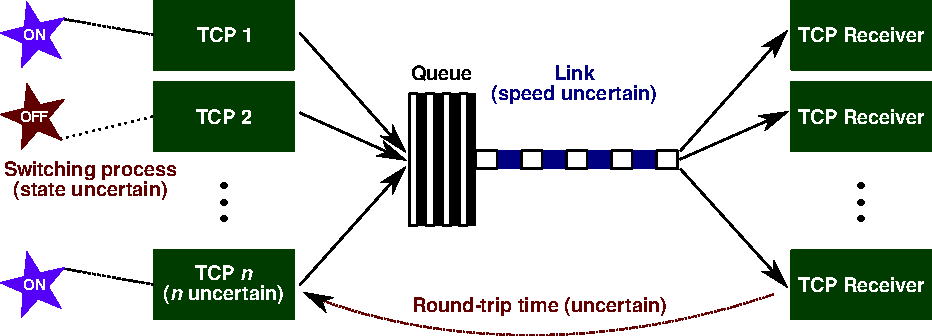
\includegraphics[width=\columnwidth]{dumbbell.pdf}
\caption{Dumbbell network with uncertainty.}
\label{fig:dumbbell}

\end{figure}

A single evaluation step consists of drawing somewhere between 16 and
100 network specimens from the network model, then simulating the
RemyCC algorithm at each sender an extended length of time on each
network specimen. At the end of the simulation, the objective function
for each sender, given by Equation~\ref{eq:util}, is totaled to
produce an overall figure of merit for the RemyCC. We explore two
cases, $\alpha = \beta = 1$ and $\alpha=2, \delta = 0$. The first case
corresponds to proportional throughput and delay fairness,
maximizing $$U = \log (\mbox{throughput}) - \delta \cdot \log
(\mbox{delay}),$$ with $\delta$ specifying the importance placed on
delay vs.~throughput. The second case corresponds to minimizing the
potential delay of a fixed-length transfer, by maximizing $$U =
-\frac{1}{\mbox{throughput}}.$$

%\subsection{The optimization procedure}

Remy initializes a RemyCC with only a single rule. Any values of the
state variables (between 0 and 16,384) are mapped to a default action
where $m = 1$, $b = 1$, $r = 0.01$.

Each entry in the rule table has an ``epoch.''
Remy maintains a global epoch number, initialized to 0. Remy's search
for the ``best'' RemyCC given a network model is a series of greedy
steps to build and improve the rule table:

\begin{enumerate}

\item\textbf{Set all rules to the current epoch.} 

\item \textbf{Find the most-used rule in this epoch.} Simulate the
  current RemyCC and see which rule in the current epoch
  receives the most use.  If no such rules were used, go
  to step 4.

\item \textbf{Improve that action until we can't anymore.} Focus on
  this rule and find the best action for it. Draw at least 16 network
  specimens from the model, and then evaluate roughly 100 candidate
  increments to the current action, increasing geometrically in
  granularity as they get further from the current value. For example,
  evaluate $r \pm 0.01$, $r \pm 0.08$, $r \pm 0.64$, \ldots, taking
  the Cartesian product with the alternatives for $m$ and $b$.

  The modified action is evaluated by substituting it \emph{into all
    senders} and repeating the simulation in parallel. We use the same
  random seed and the same set of specimen networks in the simulation of
  each candidate action to reduce the effects of random variation.

  If any of the candidates is an improvement, replace the action with
  the best new action and repeat the search, still with the same
  specimen networks and random seed. Otherwise, increment the epoch
  number of the current rule and go back to step~2.

\item \textbf{If we run out of rules in this epoch.} Increment the
  global epoch. If the new epoch is a multiple of a parameter, $K$,
  continue to step 5. Otherwise go back to step 1. We use $K = 4$ to
  balance structural improvements vs.~honing the existing structure.

\item \textbf{Subdivide the most-used rule.} Recall that each rule
  represents a mapping from a rectangular region of memory space to a
  single action. In this step, find the most-used rule, and the median
  memory value that triggers it. Split the rule at this point,
  producing eight new rules (one per dimension of the memory-space),
  each with the same action as before. Then return to step 1.

\end{enumerate}

By repeating this procedure, the structure of a RemyCC's rule table
becomes an octree~\cite{octree} or hextree of memory regions. Areas of
the memory space more likely to occur receive correspondingly more
attention from the optimizer, and are subdivided into smaller bins
that yield a more granular function relating memory to
action. \emph{Which} rules are more often triggered depends on every
endpoint's behavior as well as the network's parameters, so the task
of finding the right structure for the rule table is best run
alongside the process of optimizing existing rules.

%To the best of our knowledge, this dynamic partitioning approach is
%novel in the context of multi-agent optimization. The ``greedy''
%approach in step 2 is key to the computational tractability and
%efficiency of the search because it allows us to prune the search
%space. Dividing the memory space into cells of different size
%proportional to their activity produces a rule table
%whose granularity is finer in regions of higher use.

\section{Evaluation}
\label{remy:eval}

We used ns-2 to evaluate the algorithms generated by Remy and compare
them with several other congestion-control methods, including both
end-to-end schemes and schemes with router assistance. This section
describes the network and workload scenarios and our findings.

\subsection{Simulation setup and metrics}

\noindent {\bf Congestion-control protocols.} The end-to-end schemes
we compared with are NewReno, Vegas, Cubic, and Compound. In addition,
we compared against two schemes that depend on router assistance: XCP,
and Cubic over stochastic fair queueing~\cite{sfq} with each queue
running CoDel~\cite{CoDel}. We use Nichols's published sfqCoDel
implementation (version released in March 2013) for
ns-2.\footnote{\url{http://www.pollere.net/Txtdocs/sfqcodel.cc}} The
Cubic, Compound, and Vegas codes are from the Linux implementations
ported to ns-2 and available in ns-2.35.  For the datacenter
simulation, we also compare with the DCTCP ns-2.35
patch.\footnote{\url{http://www.stanford.edu/~alizade/Site/DCTCP.html}}

{\bf RemyCCs.} We used Remy to construct three general-purpose
RemyCCs. Each one was designed for an uncertain network model with the
dumbbell topology of Figure~\ref{fig:dumbbell}, but with three
different values of $\delta$ (the relative importance of delay): 0.1,
1, and 10. The parameters of the network and traffic model used at
design time were:

\vspace{\baselineskip}

\begin{tabular}{lll}
\bf Quantity & \bf Design range & \bf Distribution \\
\hline $n$ max senders & 1--16 & uniform \\
``on'' process & mean 5~s & exponential \\
``off'' process & mean 5~s & exponential \\
link speed & 10--20~Mbps & uniform \\
round-trip time & 100--200~ms & uniform \\
queue capacity & unlimited & \\
\end{tabular}

\vspace{\baselineskip}

The model captures a 64-fold range of bandwidth-delay product per
user. Each RemyCC took about 3--5 CPU-days to optimize. Calculations
were run on Amazon EC2 and on an 80-core and 48-core server at MIT. In
wall-clock time, each RemyCC took a few hours to be constructed.
The RemyCCs contain between 162 and 204 rules each.

We also used Remy to assess how performance varies based on the
specificity of the assumptions used at design time, by building
one RemyCC for a link speed known exactly \emph{a priori}, and
one that assumes only that the link speed will lie within a tenfold range:

\vspace{\baselineskip}

\begin{tabular}{lll}
\bf Quantity & \bf Design range & \bf Distribution \\
\hline $n$ max senders & 2 & uniform \\
``on'' process & mean 5~sec & exponential \\
``off'' process & mean 5~sec & exponential \\
link speed & 15~Mbps (``$1\times$'') & exact \\
link speed & 4.7--47~Mbps (``$10\times$'') & uniform \\
round-trip time & 150~ms & exact \\
queue capacity & unlimited & \\
\end{tabular}

\vspace{\baselineskip}

In most experiments, all the sources run the same protocol; in some,
we pick different protocols for different sources to investigate how
well they co-exist. Each simulation run is generally 100 seconds long,
with each scenario run at least 128 times to collect summary
statistics.

\begin{figure}
%\vspace{\baselineskip}
\begin{centering}
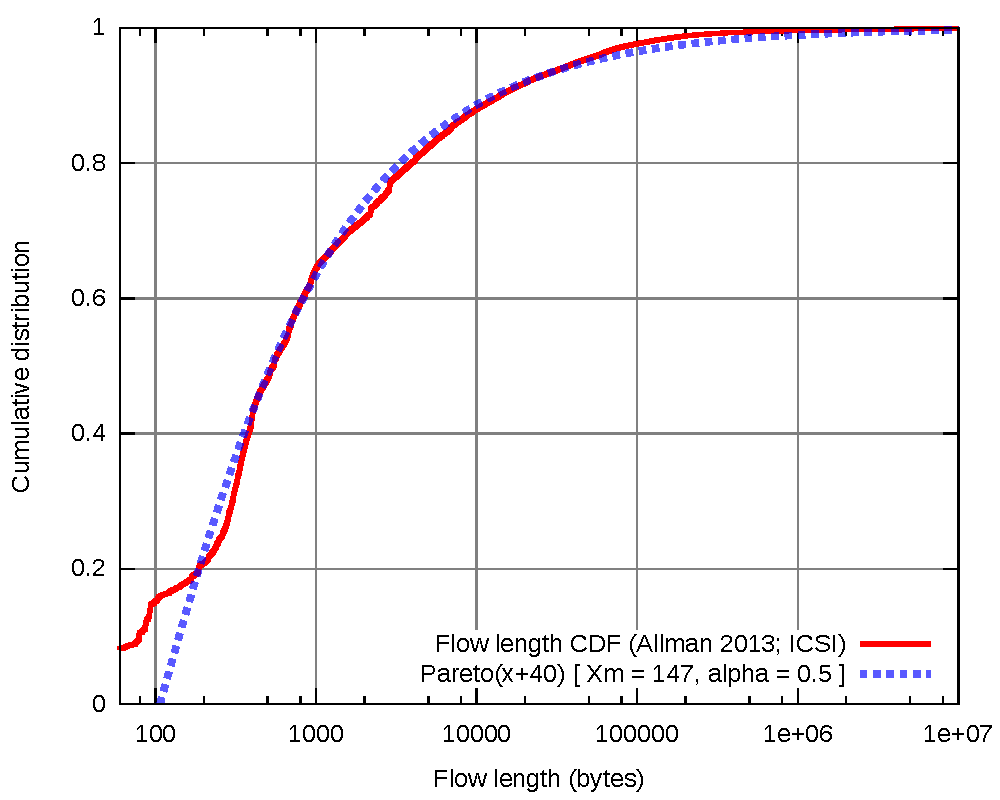
\includegraphics[width=\columnwidth]{flowlength.pdf}
\end{centering}
\caption{Observed Internet flow length distribution matches a Pareto ($\alpha = 0.5$)
distribution, suggesting mean is not well-defined.}
\label{f:flowcdf}
\end{figure}

\medskip
\noindent
{\bf Workloads.} Each source is either ``on'' or ``off'' at any point
in time. In the evaluation, we modeled the ``off'' times as exponentially distributed, and
the ``on'' distribution in one of three different ways:
\begin{itemize}
\item {\em by time}, where the source sends as many bytes as the
  congestion-control protocol allows, for a duration of time picked
  from an exponential distribution,
\item {\em by bytes}, where the connection sends as many bytes as
  given by an exponential distribution of a given average and shape,
  and
\item {\em by empirical distribution}, using the flow-length CDF from
  a large trace captured in March 2012 and published
  recently~\cite{allman-ccr-trace}. The flow-length CDF matches a
  Pareto distribution with the parameters given in
  Figure~\ref{f:flowcdf}, suggesting that the underlying distribution
  does not have finite mean. In our evaluation, we add 16 kilobytes to
  each sampled value to ensure that the network is loaded.
\end{itemize}

\medskip
\noindent {\bf Topologies.} We used these topologies in our experiments:
\begin{enumerate}
\item {\bf Single bottleneck (``dumbbell''):} The situation in
  Figure~\ref{fig:dumbbell}, with a 1,000-packet buffer, as might be
  seen in a shared cable-modem uplink. We tested a configuration whose
  link speed and delay were within the RemyCC design ranges:

%\vspace{\baselineskip}

\begin{tabular}{lll}
\bf Quantity & \bf Range & \bf Distribution \\
\hline link speed & 15~Mbps & exact \\
round-trip time & 150~ms & exact \\
queue capacity & 1000 pkts (tail drop) \\
\end{tabular}

\item {\bf Cellular wireless:} We measured the downlink capacity of the
  Verizon and AT\&T LTE cellular services while mobile, by carefully
  saturating the downlink (without causing buffer overflow) and
  recording when packets made it to the user device. We recreate this
  link within ns-2, queueing packets until they are released to the
  receiver at the same time they were released in the trace. This
  setup probes the RemyCC's resilience to ``model mismatch'' --- in
  both the Verizon and AT\&T traces, throughput and round-trip time
  were outside the limits of the RemyCC design range.
  
%\vspace{\baselineskip}

\begin{tabular}{lll}
\bf Quantity & \bf Range & \bf Distribution \\
\hline link speed & varied 0--50~Mbps & empirical \\
round-trip time & 50~ms & exact \\
queue capacity & 1000 pkts (tail drop) \\
\end{tabular}

\item {\bf Differing RTTs:} Cases where different RemyCCs, contending for
  the same link, had different RTTs to their corresponding
  receiver. We analyzed these cases for throughput and delay fairness
  and compared with existing congestion-control schemes.

\begin{tabular}{lll}
\bf Quantity & \bf Range & \bf Distribution \\
\hline $n$ max senders & 4 \\
``on'' process & $16 \times 10^3$--$3.3 \times 10^9$ bytes & Fig.~\ref{f:flowcdf}\\
``off'' process & mean 0.2~sec & exponential \\
link speed & 10~Mbps & exact \\
queue capacity & 1000 pkts (tail drop) \\
\end{tabular}

\item {\bf Datacenter:} We compared a RemyCC against
  DCTCP in a simulated datacenter topology.

\begin{tabular}{lll}
\bf Quantity & \bf Range & \bf Distribution \\
\hline $n$ max senders & 64 & exact \\
``on'' process & mean 20 megabytes & exponential \\
``off'' process & mean 0.1~sec & exponential \\
link speed & 10~Gbps & exact \\
round-trip time & 4~ms & exact \\
queue capacity & 1000 pkts (tail drop) & (for RemyCC) \\
queue capacity & modified RED & (for DCTCP) \\
\end{tabular}

\end{enumerate}

In addition, we investigate:
\begin{enumerate} 
\item[5.] {\bf Competing protocols:} We assessed how a RemyCC ``played with''
  existing congestion-control schemes (Cubic and Compound) when contending
  for the same bottleneck link.
\item [6.] {\bf Sensitivity of design range:} We investigated how
  helpful prior knowledge of the network is to the performance of
  Remy's generated algorithms.
\end{enumerate}


\medskip
\noindent {\bf Metrics.}  We measure the throughput and average
queueing delay observed for each source-destination pair. With an
on-off source, measuring throughput takes some care.  We define the
throughput of a pair as follows. Suppose the pair is active during
(non-overlapping) time intervals of length $t_1, t_2, \ldots$ during
the entire simulation run of $T$ seconds. If in each interval the
protocol successfully receives $s_i$ bytes, we define the throughput
for this connection as $\sum s_i / \sum t_i$.%  Of course, this
%throughput cannot exceed the bottleneck link rate.

We are interested in the end-to-end delay as well; the reasoning
behind Remy's objective function and the $\delta$ parameter is that
protocols that fill up buffers to maximize throughput are not as
desirable as ones that achieve high throughput \emph{and} low delay
--- both for their effect on the user, who may prefer to get his
packets to the receiver sooner, as well as any other users who share
the same FIFO queue.

We present the results for the different protocols as {\bf
  throughput-delay plots}, where the log-scale $x$-axis is the
queueing delay (average per-packet delay in excess of minimum
RTT). Lower, better, delays are to the right.  The $y$-axis is the
throughput. Protocols on the ``top right'' are the best on such
plots. We take each individual 100-second run from a simulation as one
point, and then compute the 1-$\sigma$ elliptic contour
of the maximum-likelihood 2D Gaussian distribution that explains the
points. To summarize the whole scheme, we plot the median per-sender
throughput and queueing delay as a circle.

Ellipses that are narrower in the throughput or delay axis correspond
to protocols that are fairer and more consistent in allocating those
quantities. Protocols with large ellipses --- where
identically-positioned users differ widely in experience based on the
luck of the draw or the timing of their entry to the network --- are
less fair. The orientation of an ellipse represents the {\em
  covariance between the throughput and delay} measured for the
protocol; if the throughput were uncorrelated with the queueing delay
(note that we show the queueing delay, not the RTT), the ellipse's
axes would be parallel to the graph's.
Because of the variability and correlations between these quantities
in practice, we believe that such throughput-delay plots are an
instructive way to evaluate congestion-control protocols; they provide
more information than simply reporting mean throughput and delay values.

\subsection{Single Bottleneck Results}

We start by investigating performance over the simple, classic
single-bottleneck ``dumbbell'' topology.  Although it does not model
the richness of real-world network paths, the dumbbell is a valuable
topology to investigate because in practice there are many
single-bottleneck paths experienced by Internet flows.

\begin{figure}
%\vspace{\baselineskip}
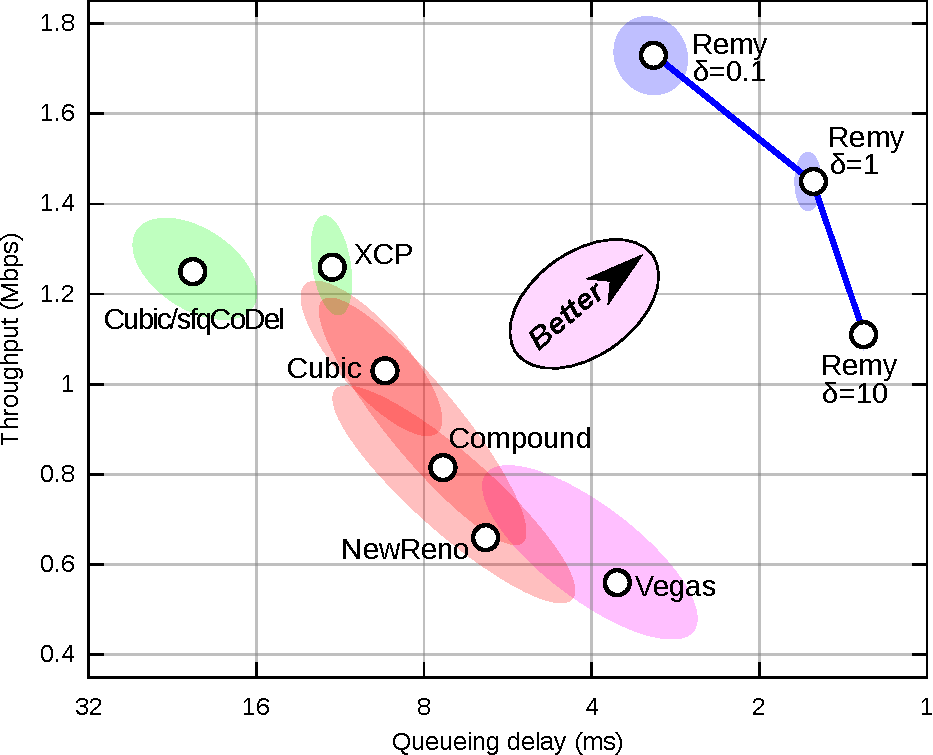
\includegraphics[width=\columnwidth]{eth8-final-bytes.pdf}
\caption{Results for each of the schemes over a 15~Mbps dumbbell
  topology with $n = 8$ senders, each alternating between flows of
  exponentially-distributed byte length (mean 100 kilobytes) and
  exponentially-distributed off time (mean 0.5 s). Medians and
  1-$\sigma$ ellipses are shown. The blue line represents the
  efficient frontier, which here is defined entirely by
  the RemyCCs.}

\label{f:tpdelaydb4}

\end{figure}

\begin{figure}
%\vspace{\baselineskip}
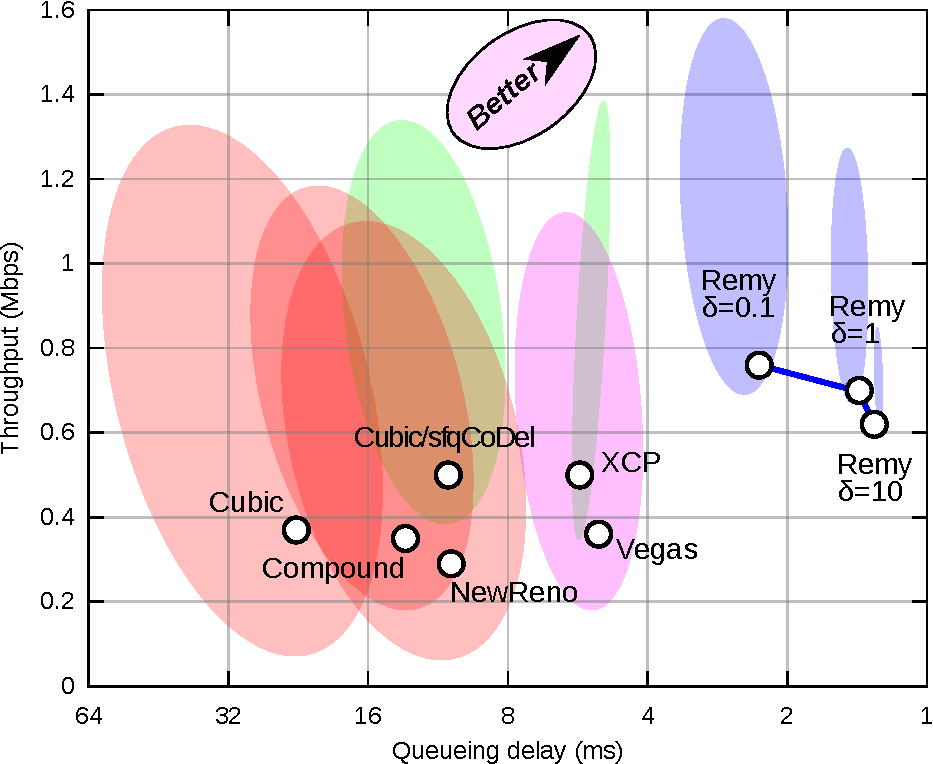
\includegraphics[width=\columnwidth]{eth12-final-flowcdf.pdf}
\caption{Results for the dumbbell topology with $n = 12$ senders, each
  alternating between flows whose length is drawn from the ICSI trace
  (Fig.~\ref{f:flowcdf}) and exponentially-distributed off time (mean
  = 0.2 s). Because of the high variance of the sending distribution,
  $\frac{1}{2}$-$\sigma$ ellipses are down. The RemyCCs again mark
  the efficient frontier.}

\label{f:tpdelaydb8}


\end{figure}

Recall that this particular dumbbell link had most of its parameters
found inside the limits of the design range of the RemyCCs
tested. As desired, this test demonstrates that Remy was successful in
producing a family of congestion-control algorithms for this type of
network.

Results from the 8-sender and 12-sender cases are shown in
Figures~\ref{f:tpdelaydb4} and \ref{f:tpdelaydb8}. RemyCCs are shown
in light blue; the results demonstrate the effect of the $\delta$
parameter in weighting the cost of delay. When $\delta = 0.1$, RemyCC
senders achieve greater median throughput than those of any other scheme,
and the lowest delay (other than the two other RemyCCs). As $\delta$
increases, the RemyCCs trace out an achievability frontier of the
compromise between throughput and delay. In this experiment, the
computer-generated algorithms outperformed all the human-designed ones.

From right to left and bottom to top, the end-to-end TCP
congestion-control schemes trace out a path from most delay-conscious
(Vegas) to most throughput-conscious (Cubic), with NewReno and Compound
falling in between.

The schemes that require in-network assistance (XCP and
Cubic-over-sfqCoDel, shown in green) achieve higher throughput than
the TCPs, but less than the two more throughput-conscious
RemyCCs.\footnote{It may seem surprising that sfqCoDel, compared with
  DropTail, \emph{increased} the median RTT of TCP Cubic. CoDel drops
  a packet at the front of the queue if all packets in the past 100~ms
  experienced a queueing delay (sojourn time) of at least 5~ms. For
  this experiment, the transfer lengths are only 100~kilobytes; with a
  500 ms ``off'' time, such a persistent queue is less common even
  though the mean queueing delay is a lot more than 5 ms. DropTail
  experiences more losses, so has lower delays (the maximum queue size
  is $\approx 4\times$ the bandwidth-delay product), but also lower
  throughput than CoDel. In other experiments with longer transfers,
  Cubic did experience lower delays when run over sfqCoDel instead of
  DropTail.} This result is encouraging, because it suggests that even
a purely end-to-end scheme can outperform well-designed algorithms
that involve active router participation.  This demonstrates that
distributed congestion-control algorithms that explicitly maximize
well-chosen objective functions can achieve gains over existing
schemes.  As we will see later, however, this substantially better
performance will not hold when the design assumptions of a RemyCC are
contradicted at runtime.

In Figures~\ref{f:tpdelaydb4} and \ref{f:tpdelaydb8}, the RemyCCs do
not simply have better median performance --- they are also more fair
to individual flows, in that the performance of an individual sender
(indicated by the size of the ellipses) is more consistent in both
throughput and delay.

\begin{figure}
%\vspace{\baselineskip}
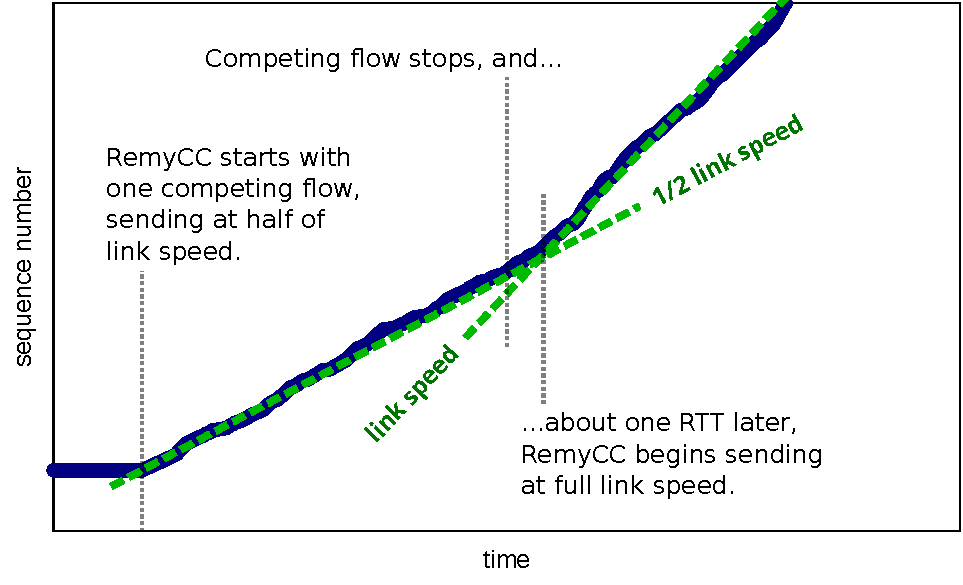
\includegraphics[width=\columnwidth]{trace.pdf}
\caption{Sequence plot of a RemyCC flow in contention with varying
  cross traffic. The flow responds quickly to the departure of a
  competing flow by doubling its sending rate.}
\label{f:trace}
\end{figure}

To explain this result, we investigated how multiple RemyCC flows
share the network. We found that when a new flow starts, the system
converges to an equitable allocation quickly, generally after little
more than one RTT. Figure~\ref{f:trace} shows the sequence of
transmissions of a new RemyCC flow that begins while sharing the link.
Midway through the flow, the competing traffic departs, allowing
the flow to start consuming the whole bottleneck rate.

\begin{figure}
%\vspace{\baselineskip}
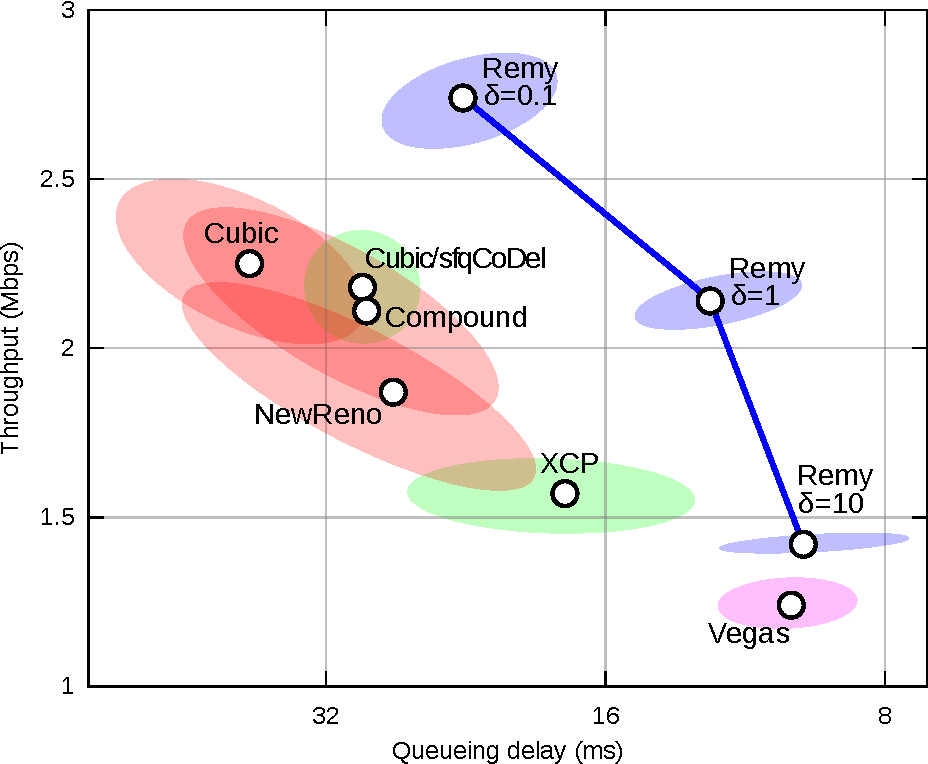
\includegraphics[width=\columnwidth]{vzw-4-final.pdf}
\caption{Verizon LTE downlink trace, $n = 4$. 1-$\sigma$ ellipses are shown.
The RemyCCs define the efficient frontier. Senders alternated between
exponentially-distributed file transfers (mean 100 kilobytes) and
exponentially-distributed pause times (mean 0.5 s).}
\label{f:verizon4}

\end{figure}

\begin{figure}
%\vspace{\baselineskip}
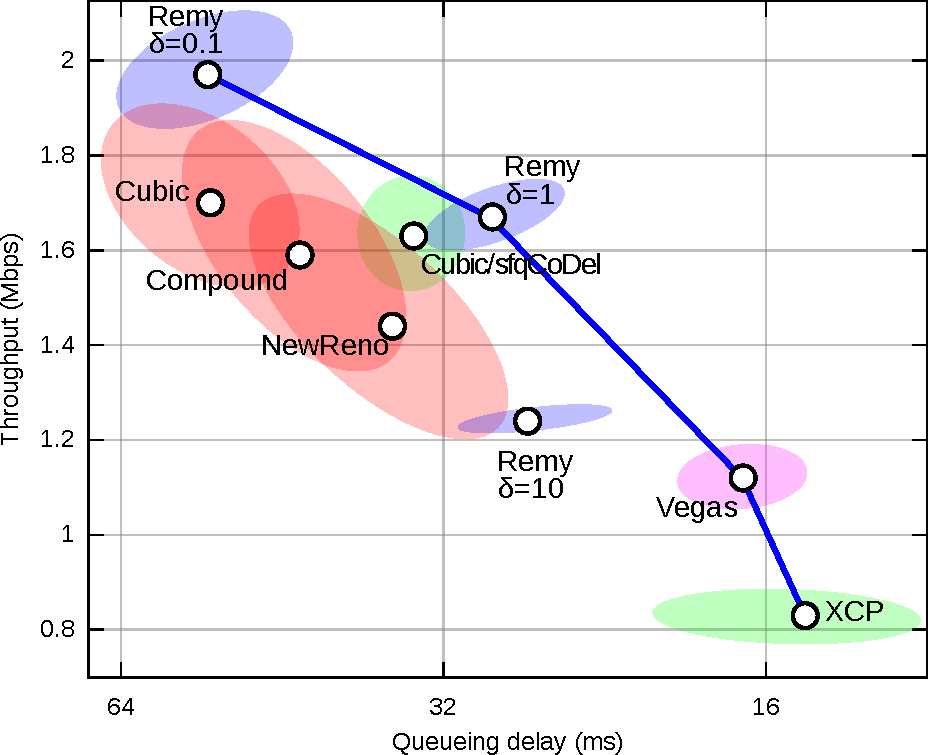
\includegraphics[width=\columnwidth]{vzw-8-final.pdf}
\caption{Verizon LTE downlink trace, $n = 8$. 1-$\sigma$ ellipses are
  shown.  As the degree of multiplexing increases, the schemes move
  closer together in performance and router-assisted schemes begin to
  perform better. Two of the three RemyCCs are on the efficient frontier.}
\label{f:verizon8}
\end{figure}

\begin{figure}
%\vspace{\baselineskip}
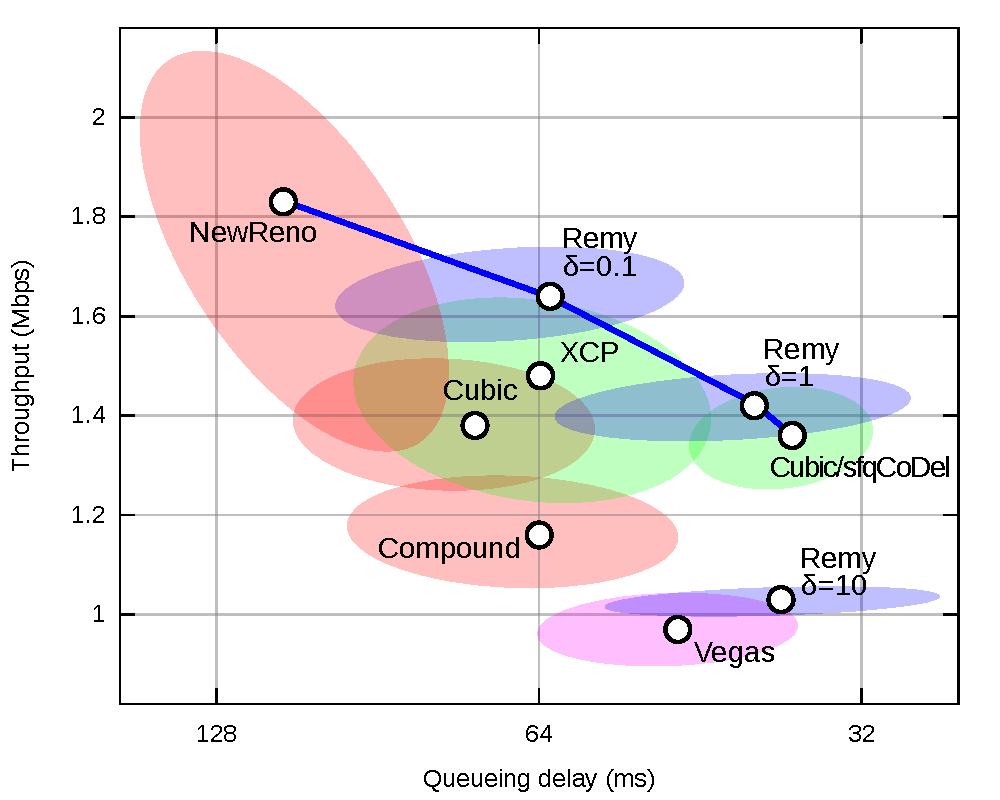
\includegraphics[width=\columnwidth]{att-4-final.pdf}
\caption{AT\&T LTE downlink trace, $n = 4$. Two of the RemyCCs are on
  the efficient frontier.}

\label{f:att2}
\end{figure}

%\pagebreak
\subsection{Cellular Wireless Links}

Cellular wireless links are tricky for congestion-control algorithms
because their link rates vary with time.\footnote{XCP, in particular,
  depends on knowing the speed of the link exactly; in our tests on cellular
  traces we supplied XCP with the long-term average link speed for
  this value.}

By running a program that attempts to keep a cellular link backlogged
but without causing buffer overflows, we measured the variation in
download speed on Verizon's and AT\&T's LTE service while mobile. We
then ran simulations over these pre-recorded traces, with the
assumption that packets are enqueued by the network until they can be
dequeued and delivered at the same instants seen in the trace.

%\begin{figure}
%\caption{Varying downlink capacity of the mobile Verizon LTE service
%  for a single user.}
%
%\label{f:celllinkvar}
%
%\vspace{\baselineskip}
%
%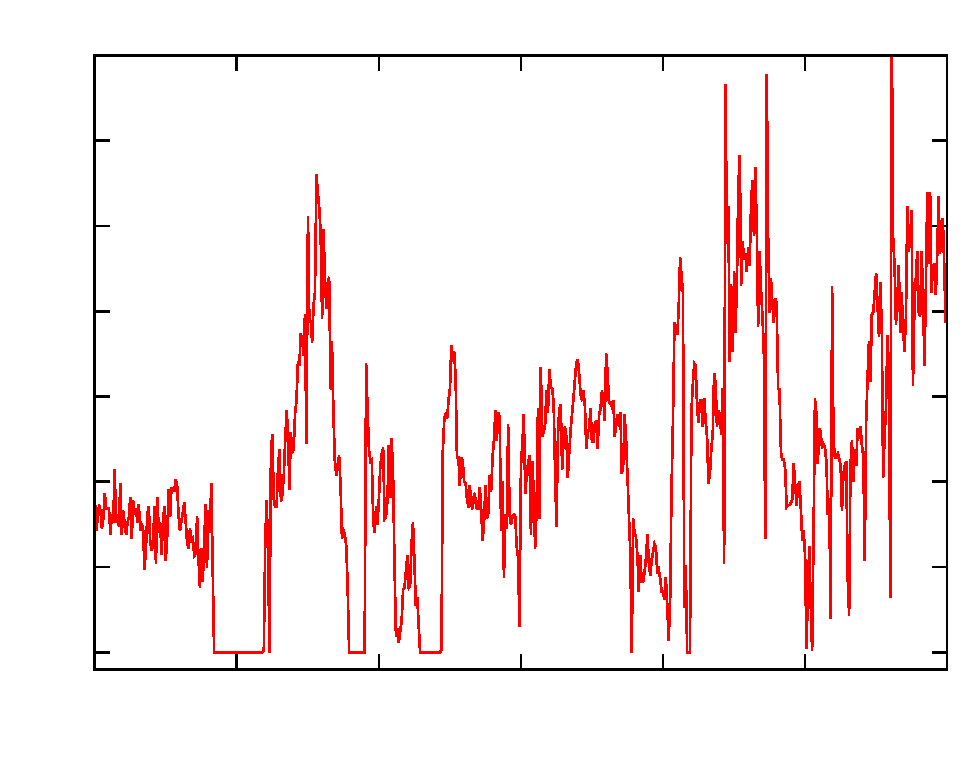
\includegraphics[width=\columnwidth]{verizon.pdf}
%
%\end{figure}

As discussed above, we did not design the RemyCCs to accommodate such a wide
variety of throughputs. Running the algorithm over this link
illustrated some of the limits of a RemyCC's generalizability beyond
situations encountered during the design phase.

Somewhat to our surprise, for moderate numbers of concurrent flows, $n
\le 8$, the RemyCCs continued to surpass (albeit narrowly) the best
human-designed algorithms, even ones benefiting from in-network
assistance. See Figures~\ref{f:verizon4} and \ref{f:verizon8}.

%However, for larger $n$, end-to-end RemyCCs no longer outperformed
%schemes with router participation. Figure~\ref{f:verizon32} shows the
%results of a simulation with $n = 32$ senders, all using the empirical
%distribution of flow lengths. The RemyCCs were no longer on the
%efficient frontier (the best schemes), although they did still
%outperform the human-designed end-to-end schemes except Vegas.

%Much further work will be necessary to assess the generalizability of
%a RemyCC. We discuss this in the next section.

%\begin{figure}
%\vspace{\baselineskip}
%\begin{centering}
%
%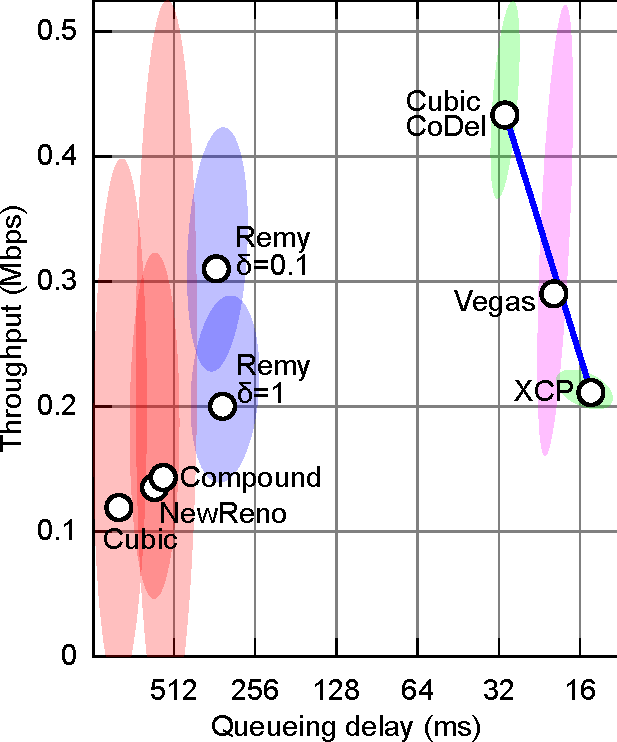
\includegraphics[width=.75\columnwidth]{verizon-32.pdf}
%
%\end{centering}

%\caption{When $n = 32$ on the Verizon trace, the RemyCCs are well
%  outside the limits of their design range of 1--16 senders. They outperform the
%  end-to-end congestion control methods except Vegas, but are beaten
%  by the in-network schemes.}

%\label{f:verizon32}
%
%\end{figure}

\subsection{Differing RTTs}

\begin{figure}
%\vspace{\baselineskip}

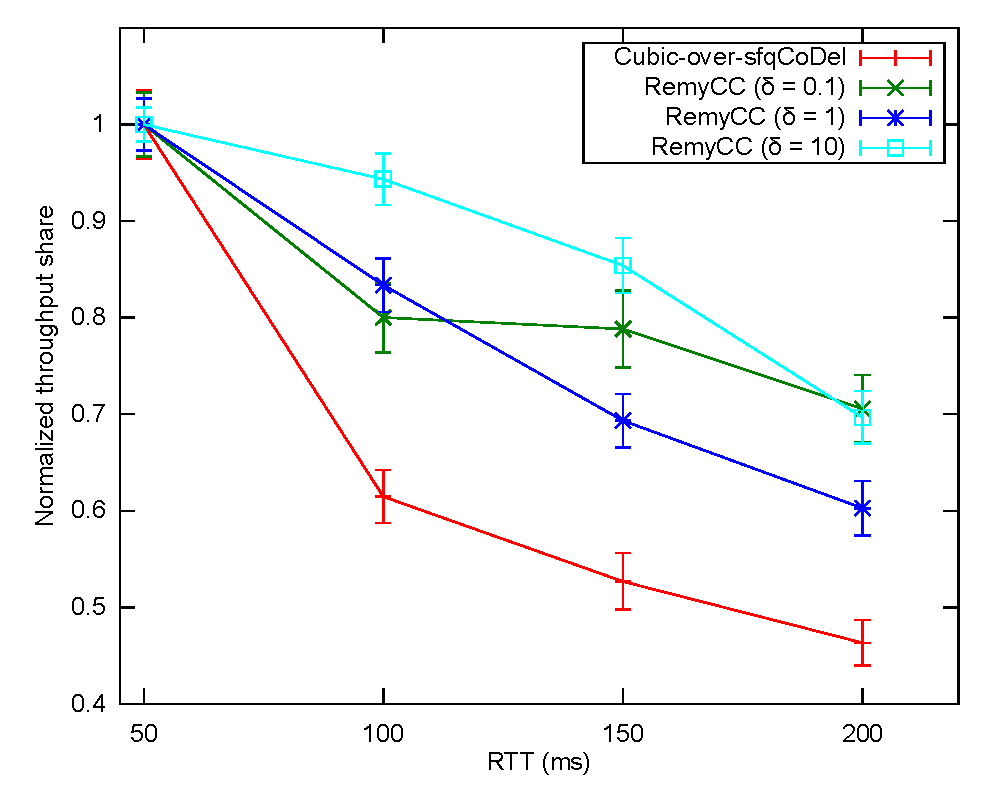
\includegraphics[width=\columnwidth]{rttfairness.pdf}
\caption{Remy's RTT unfairness compares favorably to
  Cubic-over-sfqCoDel. Error bar represents standard error of the
  mean over 128 100-second simulations.}

\label{f:fairness}

\end{figure}

We investigated how the RemyCCs allocate throughput on a contested
bottleneck link when the competing flows have different RTTs. At the
design stage, all contending flows had the same RTT (which was drawn
randomly for each network specimen from between 100~ms and 200~ms), so
the RemyCCs were not designed to exhibit RTT fairness explicitly.

We compared the RemyCCs with Cubic-over-sfqCoDel by running 128
realizations of a four-sender simulation where one sender-receiver
pair had RTT of 50~ms, one had 100~ms, one 150~ms, and one 200~ms. The
RemyCCs did exhibit RTT unfairness, but more modestly than
Cubic-over-sfqCoDel~(Fig.~\ref{f:fairness}).

\subsection{Datacenter-like topology}

We simulated 64 connections sharing a 10~Gbps datacenter link, and
compared DCTCP~\cite{dctcp} (using AQM inside the network) against
a RemyCC with a 1000-packet tail-drop queue. The RTT of
the path in the absence of queueing was 4 ms. Each sender sent 20
megabytes on average (exponentially distributed) with an ``off'' time
between its connections exponentially distributed with mean 100
milliseconds.

We used Remy to design a congestion-control algorithm to maximize
$-1/\mbox{throughput}$ (minimum potential delay) over these network
parameters, with the degree of multiplexing assumed to have been drawn
uniformly between 1 and 64.

%To do this, we simple speeded up the internal timebase of the RemyCC
%by a thousandfold. Its action variable $r$ was interpreted as a number
%of microseconds instead of milliseconds, etc. The design range of
%10--20 Mbps became a design range of 10--20 Gbps, still an order of
%magnitude away from the actual link speed.

%We compared this RemyCC with DCTCP~\cite{dctcp}, a well-known protocol
%tuned for datacenters with high bandwidths and low propagation delays
%that runs at endpoints and also inside the network.

% We found that the median DCTCP throughput averaged over 2,048
% connections was 141 Mbps, compared with 305 Mbps for the
% RemyCC. Although Remy came close to matching the human-designed
% in-network scheme, it did not outperform it in this data-center-like
% application. 

The results for the mean and median throughput (tput) for the 20 megabyte
transfers are shown in the following table:

\begin{tabular}{lll}
& \bf tput: mean, med & \bf rtt: mean, med\\
%   & ~~(Mbps) & ~~(ms)\\
\bf DCTCP (ECN) & 179, 144 Mbps & 7.5, 6.4 ms\\
\bf RemyCC (DropTail) & 175, 158 Mbps & 34, 39 ms \\
%\bf RemyCC+RED & 102,  & \\
\vspace{\baselineskip}
\end{tabular}

These results show that a RemyCC trained for the datacenter-network
parameter range achieves comparable throughput at lower variance than
DCTCP, a published and deployed protocol for similar scenarios. The
per-packet latencies (and loss rates, not shown) are higher, because
in this experiment RemyCC operates over a DropTail bottleneck router,
whereas DCTCP runs over an ECN-enabled RED gateway that marks packets
when the instantaneous queue exceeds a certain threshold. Developing
RemyCC schemes for networks with ECN and AQM is an area for future
work.

\subsection{Competing protocols}

We investigated the possibility of incremental deployment of a RemyCC,
by simulating a single bottleneck link with one RemyCC flow contending
with one flow from either Compound or Cubic, with no active queue
management. The RemyCC was designed for round-trip-times between
100~ms and 10~s, in order to accommodate a ``buffer-filling''
competitor on the same bottleneck link.

We used the same observed traffic distribution from
Figure~\ref{f:flowcdf} and varied the mean ``off'' time (exponentially
distributed) of the senders.  The bottleneck link speed was 15~Mbps
and baseline RTT was 150 ms. We also experimented with flows of mean
sizes 100 kilobytes and 1 megabyte, with an exponentially distributed mean
``off'' time of 0.5 seconds between successive flows. 

The results, shown in the two tables below, depended on the duty cycle
of the senders dictated by the mean off time (numbers in parentheses
are standard deviations).

\vspace{\baselineskip}

% \begin{tabular}{lll}
% \bf Mean off time & \bf RemyCC tput & \bf Compound tput \\
% \hline 0.2~sec & 3.8~Mbps & 3.0~Mbps \\
% 0.1 & 4.1 & 4.4 \\
% 0.01 & 0.84 & 9.2 \\
% \end{tabular}

\begin{tabular}{lll}
\bf Mean off time & \bf RemyCC tput & \bf Compound tput \\
\hline 200 ms & 2.12 (.11)~Mbps & 1.79 (.18)~Mbps \\
100 & 2.18 (.08)  & 2.75 (.27)\\
10 & 2.28 (.10) & 3.9 (.13) \\
\hline
\bf Mean size & \bf RemyCC tput & \bf Cubic tput \\
100 KBytes & 2.04 (.14) & 1.31 (.16)\\
1 MByte & 2.09 (.11) & 1.28 (.11) \\
\hline
\end{tabular}

\vspace{\baselineskip}

% \begin{tabular}{lll}
% \bf Mean off time & \bf RemyCC tput & \bf Cubic tput \\
% \hline 0.2~sec & 3.4~Mbps & 3.2~Mbps \\
% 0.1 & 2.3 & 6.1 \\
% 0.01 & 0.74 & 9.3 \\
% \end{tabular}

%0.01 & 2.32 (0.1) & 3.95 (.16)  \\
%\bf Mean size & \bf RemyCC tput & \bf Cubic tput \\
%\hline
%100 KBytes & 2.06 (.13) & 1.23 (.12)\\
%1 MByte & 2.07 (.13) & 1.27 (.09) \\
%\hline
%\end{tabular}

%\vspace{\baselineskip}

We observe that this RemyCC does well at low duty cycles because it is
able to grab spare bandwidth more quickly. At higher duty cycles (with
low mean off time), Cubic and Compound tend to grab a higher share of
the bandwidth. The results, however, are close enough that we believe
a RemyCC designed for competing with more aggressive protocols may
close the gap, while retaining high performance when competing only with
like-minded RemyCCs.

\subsection{How helpful is prior knowledge about the network?}

We investigated the performance benefit conferred by having
more-specific prior information about the network, and what happens
when that prior information is incorrect.

We used Remy to construct two additional RemyCCs, each for a network
with a known minimum RTT of 150~ms. For one RemyCC, the link speed was
assumed to be 15~Mbps exactly. A second RemyCC was designed to span
a 10$\times$ range of link speeds, from 4.7~Mbps to 47~Mbps. We also
compared against Cubic-over-sfqCoDel over this range.

The results are shown in Figure~\ref{f:spec}. On the particular link
for which the ``1$\times$'' RemyCC was designed, it performs the best,
but its performance trails off quickly around that value. Within the
range of the ``10$\times$'' RemyCC, it beats Cubic-over-sfqCoDel, but
again deteriorates when the true network violates its design
assumptions. The results show that more-specific prior knowledge is
helpful and improves performance --- when it happens to be correct.

\begin{figure}
%\vspace{\baselineskip}
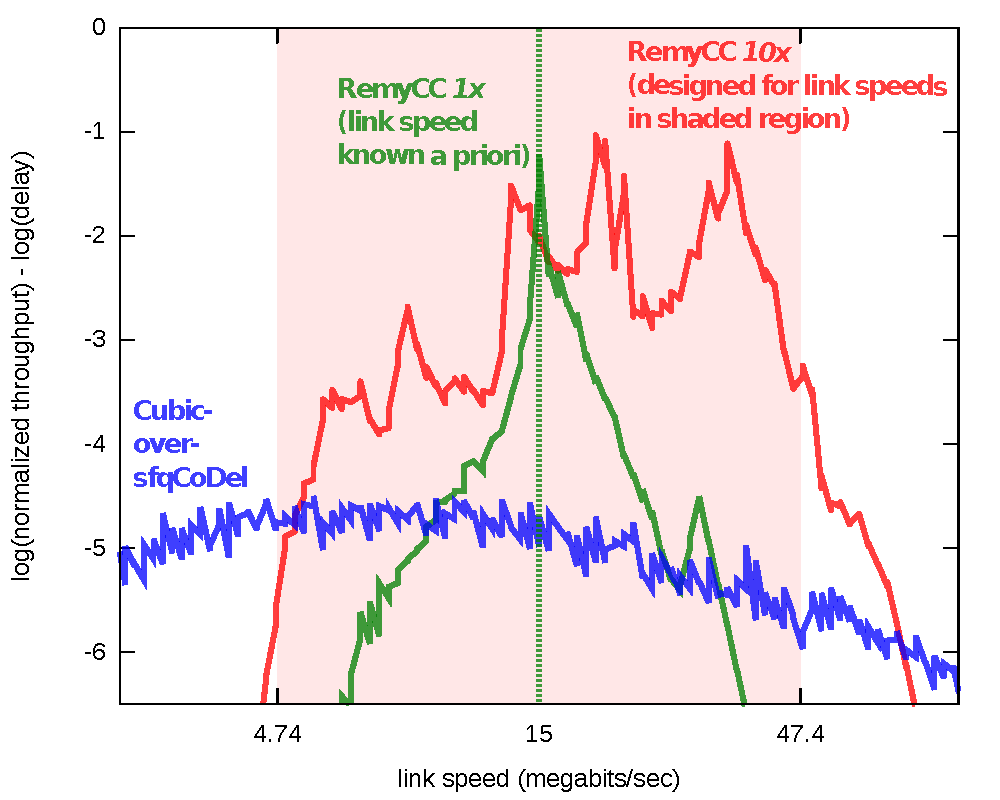
\includegraphics[width=\columnwidth]{spec2.pdf}
\caption{Performance of two end-to-end RemyCCs that were designed with
  different prior information about the network, compared with
  Cubic-over-sfqCoDel as the link speed varies. Despite running only
  at the sender, the RemyCCs each outperform Cubic-over-sfqCoDel over
  almost their entire design ranges. But when a RemyCC's
  assumptions aren't met, performance deteriorates.}

\label{f:spec}

\end{figure}

\subsection{Summary of results}

Using a few CPU-weeks of computation,
Remy produced several computer-generated congestion-control algorithms,
which we then evaluated on a variety of simulated network conditions
of varying similarity to the prior assumptions supplied at design-time.

On networks whose parameters mostly obeyed the prior knowledge
supplied at design range --- such as the dumbbell network with the
15~Mbps link --- Remy's end-to-end algorithms outperformed all of the
human-generated congestion-control algorithms, even algorithms that
receive help from network infrastructure.

RemyCC ($\delta = 0.1)$ achieved $> 1.7\times$ gains in median
throughput and $> 2.7\times$ reductions in median queueing delay
against Cubic and Compound, generally thought to be excellent
general-purpose congestion-control algorithms. Against
Cubic-over-sfqCoDel, which has the benefit of code running on network
infrastructure, RemyCC achieved a 40\% increase in median throughput
and a $7.8\times$ decrease in median queueing delay.

On the cellular link traces, which are variable and were not designed
for, Remy's schemes outperformed the existing congestion-control
algorithms (end-to-end or otherwise) when the maximum degree of
multiplexing was 4 or less, and outperformed the end-to-end schemes
and sfqCoDel when it was 8 or less. However, as the network conditions
grew farther afield from the supplied prior assumptions, Remy's
performance declined, although the algorithms were still competitive
with traditional TCP congestion control on the networks we examined.

\section{Ratatouille, a tool for understanding RemyCCs}

In our experience, high-performing computer-generated
congestion-control algorithms present a different kind of complexity
than existing mechanisms. Traditional TCP congestion control schemes
specify relatively simple rules for each endpoint, but the resulting
emergent behavior of a multiuser network is not easily specified and
can be suboptimal and unstable. By contrast, Remy's algorithms specify
hundreds of rules at the endpoints, but produce more consistent
overall behavior.

We think this tradeoff is ultimately worth taking: today's endpoints
can execute complex algorithms almost as easily as simple ones, and
the \textit{computational} complexity of a RemyCC is low in any event.

But when endpoint algorithms become so complex, it is challenging to
explain \emph{why} a particular RemyCC works without considerable
effort spent reverse-engineering it. To help with this task, I built a
visualization and debugging tool for RemyCCs, called Ratatouille.

Ratatouille displays real-time output from the Remy network simulator,
and plots the current number of packets-in-flight for each concurrent
flow as it evolves over time. The user adjusts a physical USB control
surface (a software mixing board) to vary network parameters,
including the number of flows with offered load and the link rate,
propagation delay, and buffer size at the bottleneck queue. The user
can then observe how the flows respond to the changing
conditions. Ratatouille can also run conventional AIMD TCP-like flows
for comparison.

By exploring the evolving values of the congestion signals, we have
gained some intuition into how a RemyCC can achieve good
performance. When the network is in steady state, the congestion
signals of a RemyCC sender tend to fall into an orbit, or limit cycle,
in which the average number of packets-in-flight over the cycle is
close to the ``ideal'' number: the bandwidth-delay product of the
bottleneck link divided by the degree of multiplexing.

Examining the RemyCCs that are successful in the simulations we
evaluated, we found that the period of the limit cycles is generally a
small number of minRTTs. By contrast, TCP's congestion window
generally oscillates on a much longer timescale that depends on the
buffer size, because the ``multiplicative decrease'' feature of TCP's
control rules is only triggered when packet loss is detected (in other
words, only after buffer overflow occurs in the bottleneck queue).

Our observations suggest that a RemyCC's ability to achieve better
throughput than TCP on finite-length flows is mostly due to its
quicker response to changes in conditions---a RemyCC will generally
``ramp up'' to the ideal number of packets-in-flight more quickly than
the TCP slow-start algorithm.

Although Ratatouille has allowed us to make observations that suggest
``why'' RemyCCs achieve their good performance compared with
human-designed mechanisms, much more work will be necessary before we
can reason about the performance and robustness of RemyCCs in a
rigorous way.

\begin{figure}
\caption{Ratatouille allows a user to vary network conditions on a
  physical control service, then observe the resulting behavior of a
  RemyCC in real-time.}
\label{fig:ratscreen}

\begin{center}

(XXX insert screenshot)

\end{center}
\end{figure}

\section{Conclusion}
\label{remy:concl}

This paper asks whether the design of distributed congestion-control
algorithms for heterogeneous and dynamic networks can be done by
specifying the assumptions that such algorithms are entitled to have
and the policy they ought to achieve, and letting computers work out
the details of the per-endpoint mechanisms.

Much future work remains before this question can be answered for
the real-world Internet, but our findings suggest that this approach
has considerable potential.

We developed and evaluated Remy, a program that designs end-to-end
congestion-control algorithms to human-supplied specifications. Remy's
outputs handily outperform the best-known techniques, including ones
that require intrusive in-network changes, in scenarios where network
parameters varied over one or two orders of magnitude.

Our results, and many others in the literature, indicate that there is
no existing single congestion-control method that is the best in all
situations. Moreover, the set of ``all situations'' is rapidly growing
as new subnetworks and link technologies proliferate.  A
computer-generated approach that maximizes an explicit function of the
throughput and delay to generate algorithms may be the right way
forward for the networking community.  Today's informal approach of
hampering lower layers or providing vague advice on how best to
accommodate TCP should be replaced by end-to-end algorithms (in TCP
and elsewhere) that adapt to {\em whatever} the lower layers are
doing.  Remy provides a way to achieve this goal.

\section{Acknowledgments}

We are grateful to Anirudh Sivaraman for several contributions to the
simulator and for helpful discussions. We thank Leslie Kaelbling,
Christopher Amato, Scott Shenker, and our shepherd, Ranjita
Bhagwan. We thank Frans Kaashoek and Nickolai Zeldovich for the use of
multicore machines at MIT. KW was supported by the Claude E.~Shannon Research
Assistantship. We thank the members of the MIT Center for Wireless
Networks and Mobile Computing (Wireless@MIT), including Amazon.com,
Cisco, Google, Intel, Mediatek, Microsoft, ST Microelectronics, and
Telefonica, for their support. This work was also supported in part by
NSF grant CNS-1040072.


\chapter{Using Remy to Measure the Learnability of Congestion Control}
\label{chap:learnability}

\begin{abstract}

When designing a distributed network protocol, typically it is
infeasible to fully define the target network where the protocol is
intended to be used. It is therefore natural to ask: How faithfully do
protocol designers really need to understand the networks they design
for? What are the important signals that endpoints should
listen to?  How can researchers gain confidence that systems that work
in testing scenarios will also perform adequately on real networks
that are inevitably more complex, or future networks yet to be
developed? Is there a tradeoff between the performance of a protocol
and the breadth of its intended operating range of networks? What is
the cost of playing fairly with cross-traffic that is governed by
another protocol?

We examine these questions quantitatively in the context of congestion
control, by using an automated protocol-design tool to approximate the
best possible congestion-control scheme given imperfect prior
knowledge about the network.  We found only weak evidence of a tradeoff
between operating range and performance, even when operating range was
extended to cover a thousand-fold range of link rates. We found that
it may be acceptable to simplify some characteristics of the
network---such as its topology---when modeling for design
purposes. Some other features, such as the degree of multiplexing and
the aggressiveness of contending endpoints, are important to capture
in a model.
\end{abstract}

%\section{Introduction}
\label{s:intro}

The previous chapter described the development of Remy, our automated
protocol-design tool. Remy generates congestion-control schemes from
first principles, given an uncertain model of the underlying network
and a stated application objective to pursue.

In practice, the designer of a congestion-control scheme for the
wide-area Internet cannot expect to supply a protocol-design tool with
a perfectly faithful model of the actual Internet. An actual model
will necessarily be simplified and imperfect. Nonetheless, designers
would naturally like to develop protocols that are broadly useful on
real networks.

In this chapter, we use Remy to quantify how much tolerance the
protocol designer can expect, or in other words: \emph{How easy is it
  to ``learn'' a network protocol to achieve desired goals, given a
  necessarily imperfect model of the networks where it will ultimately
  be deployed?}

Under this umbrella, we examine a series of questions about what
knowledge about the network is important when designing a
congestion-control protocol and what simplifications are acceptable:

\begin{enumerate}

\item \textbf{Knowledge of network parameters.} Is there a tradeoff
  between the performance of a protocol and the breadth of its
  intended operating range of network parameters~\cite{wroclawski}?
  Will a ``one size fits all'' protocol designed for networks spanning
  a thousand-fold range of link rates necessarily perform worse than
  one targeted at a subset of networks whose parameters can be more
  precisely defined in advance?  (\S\ref{s:oprangeperftradeoff})

\item \textbf{Structural knowledge.} How faithfully do protocol
  designers need to understand the topology of the network? What are
  the consequences of designing protocols for a simplified network
  path with a single bottleneck, then running them on networks with
  more-complicated structure?  (\S\ref{ss:topological})

\item \textbf{Knowledge about other endpoints.} In many settings, a
  newly-designed protocol will need to coexist with traffic from
  incumbent protocols. What are the consequences of designing a
  protocol with the knowledge that some endpoints may be running
  incumbent protocols whose traffic needs to be treated fairly
  (e.g.~the new protocol needs to divide a contended link evenly with
  TCP), versus a clean-slate design?  (\S\ref{s:tcpaware})

%\item \textbf{Different kinds of breadth.} Will a protocol designed
%  for a large range in one kind of network parameter (e.g., the link
%  rate) also have broad applicability when other network parameters
%  vary, such as the RTT or degree of multiplexing?  Which pairs of
%  network parameters are related in this way---such that a protocol's
%  breadth in one implies breadth in the other---and which aren't?
%  (\S\ref{ss:parameter})

%\item \textbf{Knowledge of network signals.} What kinds of congestion
%  signals are important for an endpoint to listen to? How much
%  information can be extracted from different kinds of feedback, and
%  how valuable are different congestion signals toward the protocol's
%  ultimate goals?  (\S\ref{s:signals})

\end{enumerate}

%\subsection*{RemyCCs as proxies for the best known algorithm}

Each of the above areas of inquiry is about the effect of a protocol
designer's imperfect understanding of the future network that a
decentralized congestion-control protocol will ultimately be run
over. In principle, we could quantify such an effect by evaluating, on
the actual network, the performance of the ``best possible''
congestion-control protocol designed for the imperfect network
\emph{model}, and comparing that with the best-possible protocol for
the actual network itself.

In practice, however, there is no tractable way to calculate the
optimal congestion-control protocol for a given network. Instead,
throughout this chapter we use Remy to construct achievability
results---RemyCCs---that stand in for the ``best possible'' average
performance across the range of network parameters supplied by the
designer.

We emphasize that there can be no assurance that Remy's algorithms
actually comes close to the optimal congestion-control protocols,
except to the extent that they approache analytical upper bounds on
performance and outperform existing schemes across the same networks.

\section{Summary of results}

The principal findings of these experiments are as follows:

\vspace{\baselineskip}

\noindent 
\textbf{Modeling a two-bottleneck network as a single bottleneck hurt
  performance only mildly.}  On the two-hop network of
Figure~\ref{fig:two-link}, on average we find that a protocol designed
for a simplified, single-bottleneck model of the network
underperformed by {\bf 17\%} a protocol that was designed with full
knowledge of the network's two-bottleneck structure
(Figure~\ref{f:multihop}). The simplified protocol outperformed TCP
Cubic-over-sfqCoDel by $2.75\times$ on average. In this example, full
knowledge of the network topology during the design process was not
crucial.

\vspace{\baselineskip}

\noindent 
\textbf{We found weak evidence of a tradeoff between
  operating range and performance.} We created a RemyCC designed
for a range of networks whose link rates spanned a thousand-fold range
between 1~Mbps and 1000~Mbps, as well as three other protocols that
were more narrowly-targeted at hundred-fold, ten-fold, and two-fold
ranges of link rate (Figure~\ref{fig:breadth}).

The ``thousand-fold'' RemyCC achieved close to the peak performance of
the ``two-fold'' RemyCC. Between link rates of 22--44~Mbps, the
``thousand-fold'' RemyCC achieved \textbf{within 3\% of the throughput}
of the ``two-fold'' protocol that was designed for this exact
range. However, the queueing delay of the ``thousand-fold'' protocol
was \textbf{46\% higher}, suggesting some benefit from more focused
operating conditions. It also takes Remy longer to optimize (offline)
a ``thousand-fold'' RemyCC compared with a two-fold RemyCC. In run-time
operation, the computational cost of the two algorithms is
similar.

Over the full range of 1~Mbps to 1000~Mbps, the ``thousand-fold''
RemyCC protocol matched or outperformed TCP Cubic and
Cubic-over-sfqCoDel over the entire range
(Figure~\ref{fig:breadth}). This result suggests that it may be
possible to construct ``one size fits all'' end-to-end
congestion-control protocols that outperform TCP, even when TCP is
assisted by in-network algorithms.

\vspace{\baselineskip}

\noindent \textbf{TCP-awareness hurt performance when TCP
  cross-traffic was absent, but helped dramatically when present.} We
measured the costs and benefits of ``TCP-awareness''---designing a
protocol with the explicit knowledge that it may be competing against
other endpoints running TCP, compared with a ``TCP-naive'' protocol
for a network where the other endpoints only run the same TCP-naive
protocol.

When contending only with other endpoints of the same kind, the
``TCP-naive'' protocol achieved \textbf{55\% less queueing delay} than
the TCP-aware protocol. In other words, ``TCP-awareness'' has a cost
measured in lost performance when TCP cross-traffic is absent
(Figure~\ref{fig:tcpawarehomo}).

But when contending against TCP, the ``TCP-naive'' protocol was
squeezed out by the more-aggressive cross-traffic. By contrast, the
``TCP-aware'' protocol achieved \textbf{36\% more throughput} and
\textbf{37\% less queueing delay} than the ``TCP-naive'' protocol,
and reached an equitable division of the available capacity with TCP
(Figure~\ref{fig:tcpawarehetero}).

\section{Protocol design as a problem of learnability}
\label{s: learnability}

\begin{comment}

This section discusses closely related work on congestion control and
explains how our work has an analogy with theoretical notions of
learnability.

\subsection{Congestion control}

Congestion control over packet-switched networks has been a productive
area of research since the seminal work of the 1980s, including
Ramakrishnan and Jain's DECBit scheme~\cite{decbit} and Jacobson's TCP
Tahoe and Reno algorithms~\cite{Jacobson88}. End-to-end algorithms
typically compute a congestion window or a paced transmission rate
using the stream of acknowledgments (ACKs) arriving from the
receiver. In response to congestion, inferred from packet loss or, in
some cases, rising delays, the sender reduces its window or rate;
conversely, when no congestion is perceived, the sender increases its
window or rate.

In this paper, we use the Remy~\cite{remy} protocol-design tool to
generate end-to-end Tao congestion-control schemes from first
principles. The Remy work showed that such an approach can produce
schemes whose performance is competitive with, and often out-performs,
human-generated schemes, including most varieties of TCP congestion
control, on intended target networks.

By contrast, this paper use Remy program as a tool for understanding
the nature of the problem of protocol design without being able to
fully define the intended target networks. We use the program's output
as a proxy for the ``best possible'' Tao congestion-control protocol
intended for a particular imperfect network model, and then ask how
that protocol performs on a different set of networks that varies from
the model in some respect (topology, link speed, behavior of
contending endpoints, etc.).

For reference, we also compare with the most prevalent
congestion-control protocols in wide use, including Linux's TCP
Cubic~\cite{cubic}, and the less-aggressive NewReno
algorithm~\cite{newreno}. End-to-end congestion control may be
assisted with explicit router participation; we also measure the
CoDel~\cite{CoDel} algorithm running with stochastic fair
queueing~\cite{sfq} for ``controlled delay'' at bottleneck gateways.

\subsection{Learnability}

\end{comment}

TCP congestion control was not designed with an explicit objective
function in mind. Kelly et al.~present an interpretation of TCP
congestion-control variants in terms of the implicit goals they
attempt to optimize~\cite{Kelly98}.  This line of work is known as
Network Utility Maximization (NUM); more recent work has modeled
stochastic NUM problems~\cite{stochasticnum}, where flows enter and
leave the network with time.

We extend this problem by examining the difficulty of designing a
network protocol given an \emph{imperfect} model of the network where
it will be deployed, in order to understand the inherent difficulties
of the problem of congestion control.

\begin{comment}
Formally speaking, designing such a protocol is a problem in
sequential decision-making under uncertain and can be modeled as a
Partially-Observable Markov Decision Process~\cite{pomdp}. In that
context, the purpose of this paper is to ask: how well can a protocol
designer ``learn'' the solution to one POMDP or set of networks and
successfully apply the result (a protocol) to a different set of networks?
\end{comment}

In doing so, we draw an explicit analogy to the concept of
``learnability'' employed in machine
learning~\cite{learnable,schapire}. A canonical machine-learning
problem attempts to design a classifier for a large population of data
points, supplied with only a smaller (and possibly skewed) ``training
set'' meant to teach the classifier about the full population of
data. Subsequently, the performance of the resulting classifier is
evaluated in how well it correctly classifies points in a ``testing
set,'' generally drawn from the actual population. Learnability theory
measures the difficulty of inferring an accurate classifier for the
testing set, given a training set.

Just as a classifier design procedure may minimize the error rate or
the width of the margin as a proxy for maximizing predictive
performance on unseen inputs, the Remy tool uses an objective function
in terms of throughput and delay, averaged over the design model, as a
proxy for performance on as-yet-unseen networks.

In our work, we envision a protocol designer working to generate a
congestion-control protocol for a large set of real networks (e.g.,
the Internet), supplied with only an imperfect model of the range of
variation and behavior of those networks. The imperfect model is the
``training scenarios''---a model of the target networks used for design
purposes. The ``testing scenarios'' are drawn from the population of actual
target networks.

Learnability here measures the difficulty of designing an adequate
protocol for a network \emph{model}, and then deploying it on real
networks that cannot be perfectly envisioned at the time of design.


\section{Experimental Setup}

\label{s:experiment}
We describe our experimental procedure below.  First, we specify a set
of \textit{training scenarios}: a set of network configurations
(\S\ref{ss:nwkcfg}) that express the designer's imperfect model of the
network. Next, we specify an \textit{objective function}
(\S\ref{ss:objective}). The protocol-design process synthesizes a
congestion-control protocol that maximizes the value of this function,
averaged over the set of training scenarios. Finally
(\S\ref{ss:eval}), we specify a \textit{testing scenario} of network
configurations, which may be similar or dissimilar to the training
scenarios.

We evaluate the synthesized congestion-control protocol on the testing
scenario to assess the questions of this study---how easy is it to
``learn'' a network protocol to achieve desired goals, given an imperfect
model of the networks where it will ultimately be deployed?

%\S\ref{s:operational} describes homogenous experiments where the testing scenario
%differs from the training scenario in operational parameters alone (topology,
%workload, minimum RTT, and link speed), assuming that all senders in the
%network run the same congestion-control protocol. \S\ref{s:diversity} deals
%with heterogeneity and describes experiments where the testing and training
%sets contain senders running multiple congestion-control protocols.

\subsection{Training scenarios}
\label{ss:nwkcfg}
The training scenarios specify the set of network configurations that
the protocol-design process is given access to. Formally, a network
configuration specifies:

\begin{enumerate}
\item The topology: link rate and propagation delay of each link in the network.
\item The locations of senders and receivers within the topology, and the paths
      connecting the senders to the receivers.
\item A model of the workload generated by the application running
  at each endpoint. We use an on/off model for the workload, where a
  sender turns ``on'' for a certain duration (or transfer length) drawn
  from an exponential distribution, then turns ``off'' for an amount of
  time drawn from another exponential distribution before turning on
  again.
\item The buffer size and queue discipline at each gateway.
\end{enumerate}

\subsection{Objective function}
\label{ss:objective}
The objective function expresses the protocol designer's figure of
merit for the goodness of a congestion-control protocol. Many such
metrics have been proposed, including alpha-fair
throughput~\cite{Srikant}, flow completion time~\cite{dctcp},
throughput-over-delay~\cite{codelID}, or measures based on a
subjective opinion score~\cite{MOSCC}.

In this study, we specifically considered objective functions of the
form:
\begin{equation}
\log\left( \textrm{throughput} \right)  - \delta \log\left( \textrm{delay} \right)
\end{equation}

Here, ``throughput'' is the average information transmission rate of a
sender-receiver pair, defined as the total number of bytes
successfully delivered divided by the total time the sender was ``on''
and had offered load. The ``delay'' is the average per-packet delay of
packets in the connection, including propagation delay and queueing
delay. The $\delta$ factor expresses a relative preference between high throughput and low delay.

The protocol-design process works to maximize the \emph{sum} of the
objective function across all connections. The $\log$ in the objective
function expresses a preference for ``proportionally-fair'' resource
allocation---for example, it is worthwhile to cut one connection's
throughput in half, as long as this enables another connection's
throughput to be more-than-doubled.

\subsection{Protocol-design process}
\label{ss:learning}
We outline the Remy protocol-design tool briefly here, following the
treatment of~\cite{remy}. Remy models a congestion-control protocol as
a set of match-action rules, mapping between the state maintained by
the sender and an action to be executed. The ``state'' tracks a small
set of congestion signals, updated on every acknowledgment from the
receiver. The ``action'' specifies changes in the behaviour of the
congestion-control protocol.

To simplify learning, Remy assumes a piecewise-constant mapping, and
searches for the mapping that maximizes the average value of the
objective function across the training scenarios.  The mapping is
initialized to prescribe a default action for all memory values. Remy
then simulates the protocol on the training scenarios and uses the
simulation results---and the resulting value of the objective
function---to gradually refine the mapping.

For the experiments in this paper, the sender tracks four
congestion signals:
\begin{enumerate}
\item \texttt{rec\_ewma}: An exponentially-weighted moving average, or
  EWMA, of the interarrival times between acks with a weight of 1/8
  for new samples.
\item \texttt{slow\_rec\_ewma}: The same, but with a weight of 1/256
  for new samples, producing an average taken over a longer history.
\item \texttt{send\_ewma}: A moving average of the intersend time
  between sender timestamps echoed in the received ACKs, with a weight
  of 1/8 for new samples.
\item \texttt{rtt\_ratio}: The ratio of the most recent
  round-trip-time measurement and the minimum RTT seen so far.
\end{enumerate}

\subsection{Value of the congestion signals}

\label{s:signals}

We performed a measurement study to evaluate the value of each of
these four signals on the ultimate performance of a congestion-control
protocol. We selectively ``knocked out'' each signal in turn and
designed a new congestion-control protocol from scratch (missing that
signal), in order to observe the effect of losing the signal on the
protocol's ultimate behavior.

In our measurements, we found that each of these congestion signals
independently brought value to a congestion-control protocol. No
three-signal subset was as strong as using all four signals. The most
valuable signal---by which we mean the signal whose removal cause the
greatest harm to the ultimate performance---was the
\texttt{rec\_ewma}. This suggests that these protocols may gain
considerable value from understanding the short-term packet-arrival
dynamics at the receiver.

\subsection{The congestion response}

The action uses a window-based congestion-control protocol that
caps the number of packets in flight, with pacing to regulate the rate
at which an end host meters packets into the network. The action for
any value of the memory is a triplet that specifies:
\begin{enumerate}
\item A multiplier $m$ to the current value of the congestion window.
\item An increment $b$ to the current value of the congestion window.
\item A lower bound $\tau$ on the pacing interval between outgoing packet transmissions.
\end{enumerate}

To emphasize that the resulting protocol is a brute-force
approximation of the best algorithm for a given set of training
scenarios and objective function, we refer to such protocols as
``tractable attempts at optimal'' congestion control, or Tao
protocols.

\subsection{Evaluation procedure}
\label{ss:eval}
To measure the difficulty of learning a congestion-control protocol
with an imperfect model of the eventual network, we choose a testing
scenario of network configurations and evaluate the Tao protocol on
it. All evaluations are performed in the ns-2
simulator. Using a different simulator for training and
testing helps give confidence that the congestion-control protocols
learned are robust to quirks in a simulator implementation.

We compare the performance of Tao protocols optimized for ``accurate''
models of the network against Tao protocols optimized for various
kinds of imperfect models, in order to measure how faithfully protocol
designers need to understand the network they are designing for. We
give the training and testing scenarios in a table.

For reference, we also compare the Tao protocols with two common schemes in wide use today:

\begin{enumerate}
\item TCP Cubic~\cite{cubic}, the default congestion-control protocol in Linux
\item Cubic over stochastic fair queueing and CoDel~\cite{CoDel}, an
  active-queue-management scheme that runs on bottleneck routers and
  assists endpoints in achieving a fairer and more efficient use of
  network resources
\end{enumerate}


\section{Measuring the learnability of congestion control}
\label{s:operational}

We conducted an experimental study to examine several aspects of
congestion-control learnability, by using Remy as an instrument to ask
questions of the form: how faithfully do protocol designers really
need to understand the networks they design for? What knowledge about
the network is important to capture in a design process, and what
simplifications are acceptable?

\subsection{Knowledge of network parameters}

\label{s:oprangeperftradeoff}

We evaluated the difficulty of designing a congestion-control
protocol, subject to imperfect knowledge about the parameters of the
network.

Some congestion-control protocols have been designed for specific
kinds of networks~\cite{dctcp,westwood} or require explicit knowledge
of the link rate \emph{a priori}~\cite{xcp}. Others are intended as
one-size-fits-all solutions, including most variants of TCP.

We set out to answer a question posed in~\cite{wroclawski}: are ``one
size fits all'' protocols inherently at a disadvantage, because of a
tradeoff between the ``operating range'' of a protocol and its performance?

To quantify this, we designed four RemyCCs for training
scenarios encompassing a thousand-fold variation in link rates, a
hundred-fold variation, a ten-fold variation, and a two-fold
variation. Each range was centered on the geometric mean of 1 and
1000~Mbps (32 Mbps), and each set of training scenarios sampled 100
link rates logarithmically from the range. The training scenarios are
shown in Table~\ref{table:oprange}.

\begin{table}
\caption{Training scenarios for ``knowledge of network parameters''
  experiment, showing the effect of varying the intended link rate
  operating range. Each RemyCC was designed for a network with a single
  bottleneck, and each sender with a mean ``on'' and ``off'' time of
  1~s.}
\label{table:oprange}
\begin{center}
\begin{tabular}{l|l|l|l}
\bf RemyCC & \bf Link rates & \bf RTT & \bf Max.~number of senders \\
\hline
1000x  & 1--1000~Mbps & 150~ms & 2 \\
100x   & 3.2--320~Mbps & 150~ms & 2 \\
10x    & 10--100~Mbps & 150~ms & 2 \\
2x     & 22--44~Mbps & 150~ms & 2 \\
\end{tabular}
\end{center}
\end{table}

We tested these schemes in ns-2 by sweeping the link speed between 1
and 1000~Mbps, keeping the other details of the simulated network
identical to the training scenario. The results are shown Figure~\ref{fig:breadth}.

\begin{figure}
%\begin{subfigure}[b]{0.49\textwidth}
%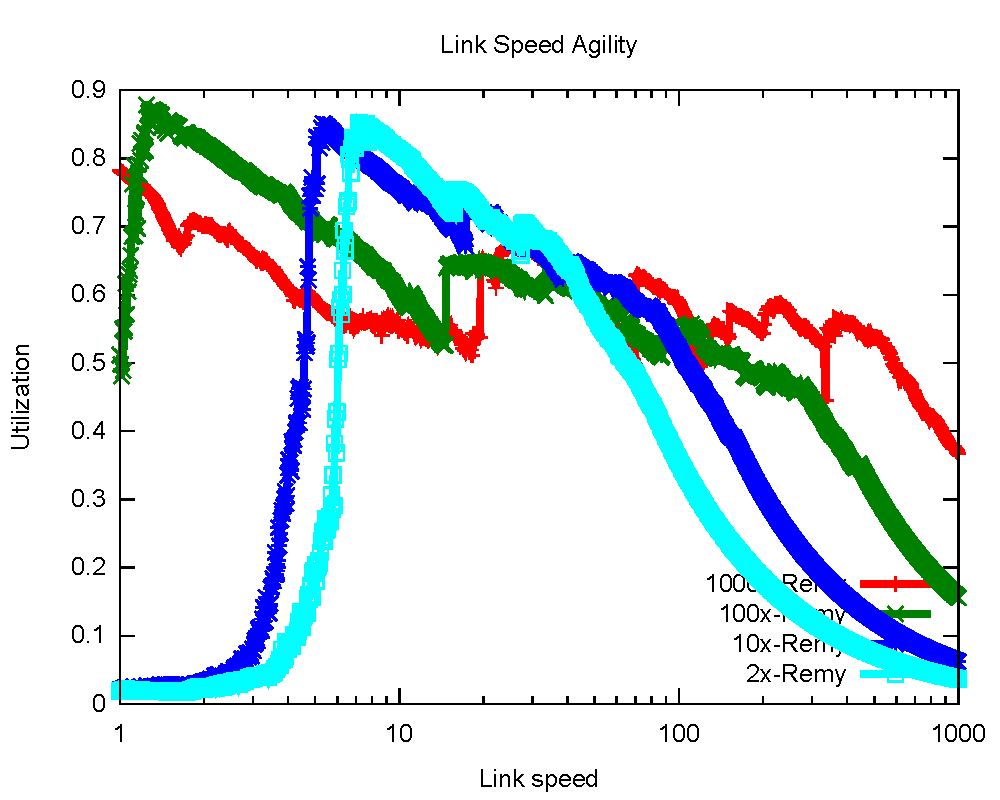
\includegraphics[width=\textwidth]{tradeoff-tpt.pdf}
%\end{subfigure}
%\begin{subfigure}[b]{0.33\textwidth}
%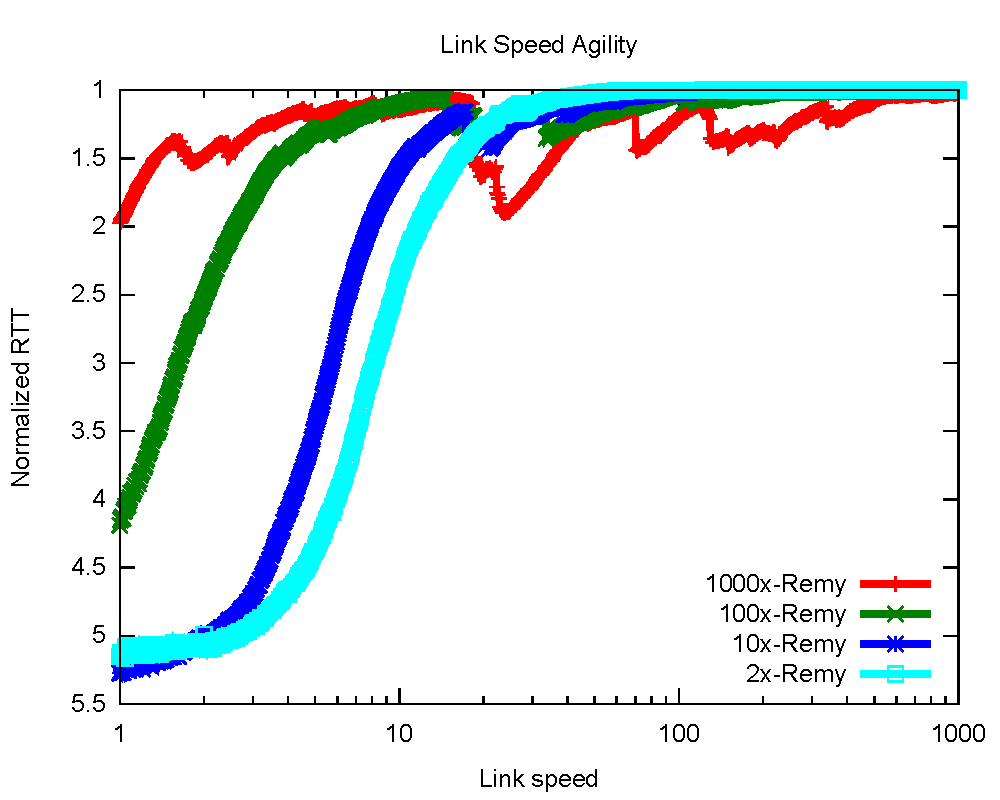
\includegraphics[width=\textwidth]{tradeoff-delay.pdf}
%\end{subfigure}
%\begin{subfigure}[b]{0.49\textwidth}
%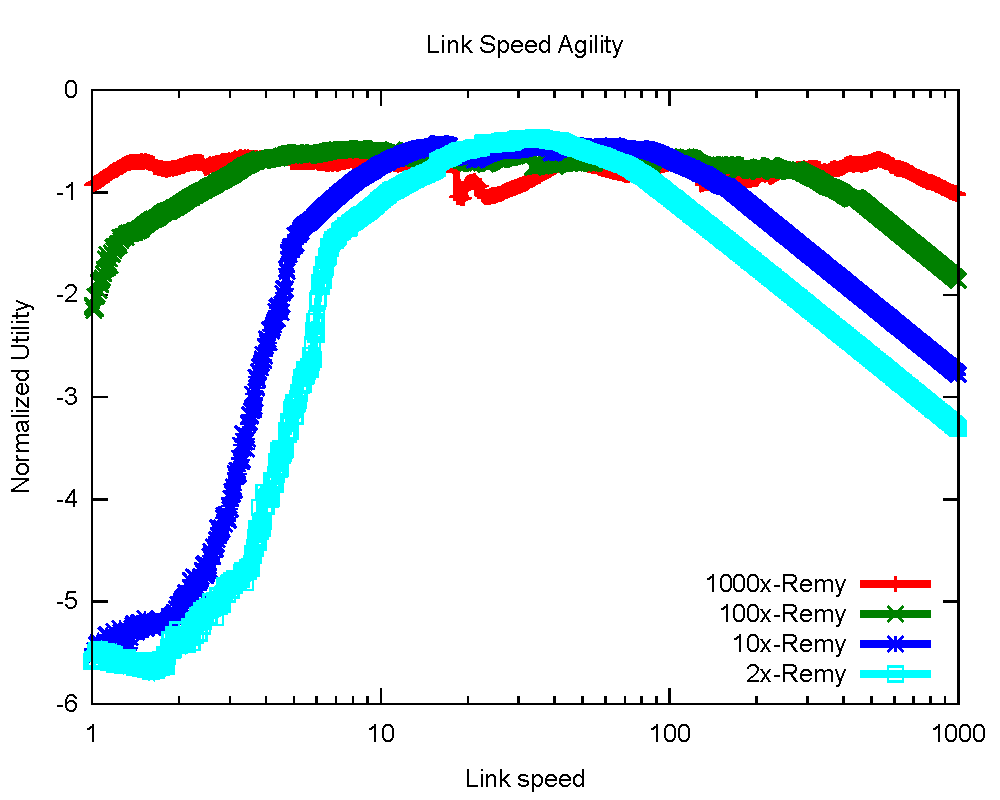
\includegraphics[width=\textwidth]{tradeoff-util.pdf}
%\end{subfigure}
\caption{Evidence of a weak tradeoff between operating range of a
  congestion-control protocol and performance. The RemyCC protocols
  designed with more specific network models (RemyCC-2x and RemyCC-10x)
  performed modestly better---within their design ranges---than protocols
  designed for a broader range of networks (RemyCC-100x and RemyCC-1000x),
  at a cost of deterioration when the actual network did not fall
  within the training scenarios. The four RemyCC protocols outperformed
  Cubic and Cubic-over-sfqCoDel over their respective design ranges.}
\label{fig:breadth}
\begin{center}
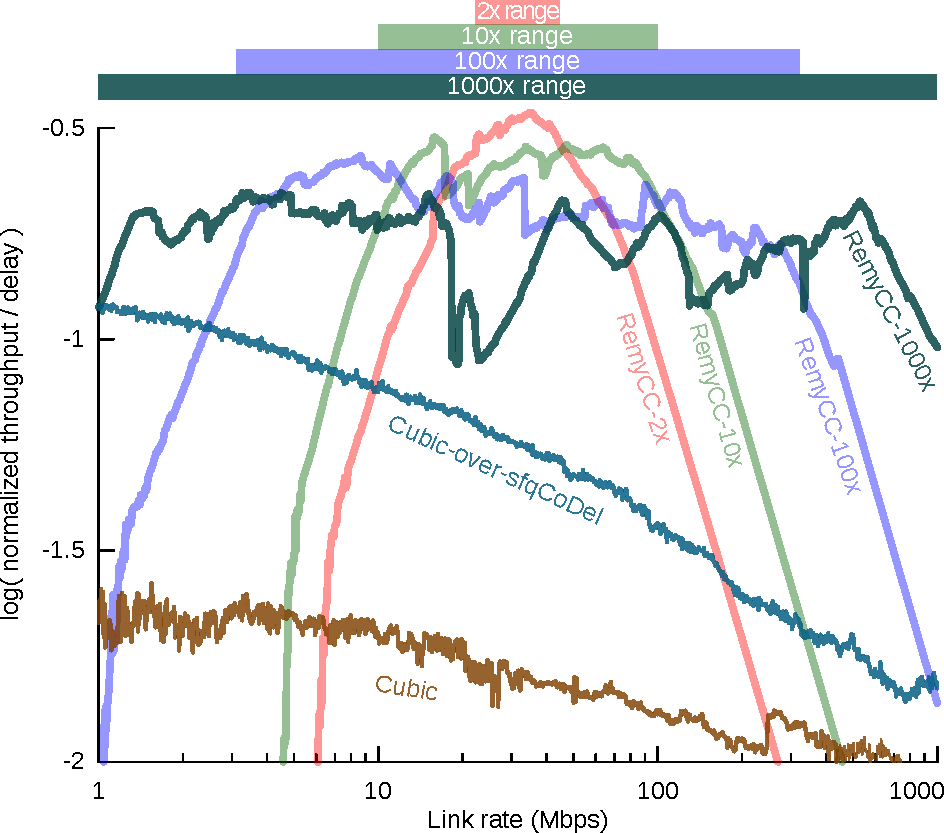
\includegraphics[width=\columnwidth]{oprange-manual.pdf}
\end{center}
\end{figure}

We found only weak evidence of a tradeoff between operating range and
performance: optimizing for a smaller range did help modestly within
that range. Because of the small magnitude of the effect, we cannot
say for sure whether simply spending more time optimizing the
broader-score RemyCCs might bring their performance closer to the
narrower-scope RemyCCs. Each RemyCC outperformed the human-designed
algorithms over its full design range, suggesting that it may be
possible to construct ``one size fits all'' RemyCCs that outperform
TCP across a broad range of real-world conditions, even when TCP is
assisted by in-network algorithms.

\subsection{Structural knowledge}
\label{ss:topological}

\begin{figure}
\caption{Parking-lot topology used to measure the consequences of imperfect
knowledge about the network's structure.}
\label{fig:two-link}
\begin{center}
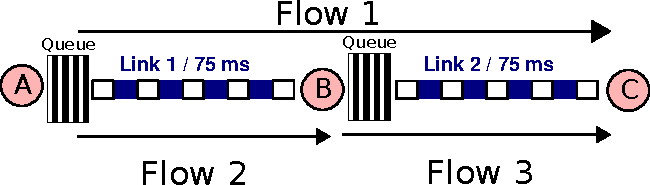
\includegraphics[width=\columnwidth]{twolink.pdf}
\end{center}
\end{figure}

We evaluated the difficulty of designing a congestion-control
protocol, subject to imperfect knowledge of the network's structure or
topology.

It is an understatement to say that the Internet is a vast network
whose full structure is known to nobody and which no model can
accurately capture. Nonetheless, researchers regularly develop new
distributed protocols for the Internet, which are deployed based on
tests in example network paths that imperfectly capture the Internet's
true complexity.

In practice, protocol designers expect that they can reason about the
performance of a distributed network algorithm by modeling the network
as something simpler than it is. We worked to capture that intuition
rigorously by studying quantitatively how difficult it is to learn a
congestion-control protocol for a more-complicated network, given a
simplified model of that network's structure.

In ns-2, we simulated a network with two bottlenecks in a
``parking-lot'' topology, shown in Figure~\ref{fig:two-link}. Flow 1
crosses both links and encounters both bottlenecks. It contends with
Flow 2 for access to the bottleneck queue and note A, and contends
with Flow 3 for access to the bottleneck queue at node B.

\begin{figure}[t!]
\caption{How well do endpoints need to understand the network around
  them? To assess this, we measure the throughput of three
  congestion-control schemes across a simulated two-hop network path,
  as the rate of each link is swept between 10 and 100~Mbps, with
  75~ms of delay per hop. A RemyCC designed for a simplified
  one-bottleneck model of the network performs 17\% worse, on average,
  than a RemyCC designed with knowledge of the network's true
  two-bottleneck structure. Both RemyCCs outperform TCP Cubic assisted
  by per-flow queueing and CoDel at the bottlenecks.}
\label{f:multihop}
\begin{center}
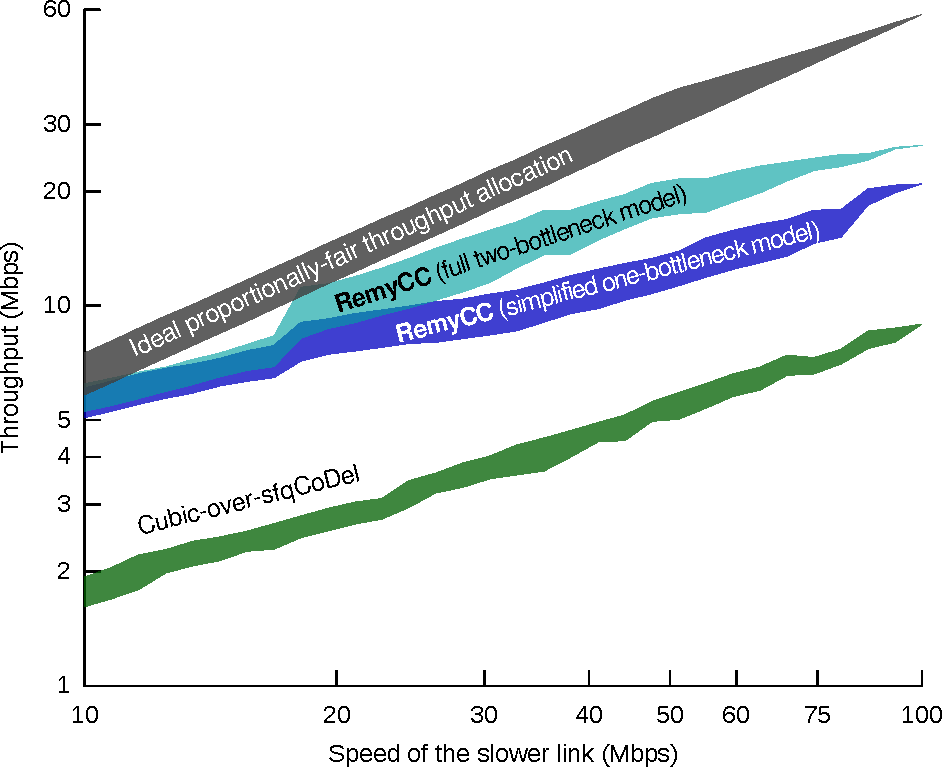
\includegraphics[width=\columnwidth]{multilink-all.pdf}
\end{center}
\end{figure}

The results for Flow 1 (the flow that crosses both links) are shown in
Figure~\ref{f:multihop}.\footnote{Results for Flow 2 and Flow 3
  (flows crossing only a single link) were nearly identical between
  the schemes.} The experiment sweeps the rate of each of the two
links between 10 and 100~Mbps, and the shaded area in the figure shows
the full locus of throughputs seen by Flow 1. For each pair of rates
(for link 1 and link 2), we also calculate the ideal
proportionally-fair throughput allocation, and plot the locus of these
points as well.

%Figure~\ref{f:multihop} shows the end-to-end throughput of connections
%traversing two bottleneck links for different protocols, including two
%RemyCCs. In each experiment, there were three flows: one that
%traversed two hops (the measured connection), a cross-traffic flow
%that traversed only the first bottleneck, and another cross-traffic
%flow that traversed only the second bottleneck.

%of two Tao protocols, running over a simulated two-hop network path
%and contending with cross traffic that runs over the first or
%second link only.

The RemyCC that was designed for the true network achieves close to
the ideal proportionally-fair throughput allocation across the two
links. The RemyCC that was designed for a simplified model of the
network with only one hop also performs adequately, but a little worse
than the ``true-network'' RemyCC. However, both computer-generated
protocols come closer to the ideal than contemporary protocols in wide
use, TCP Cubic~\cite{cubic}, the default TCP in Linux, running over
per-flow queueing and CoDel~\cite{CoDel}, an active queue management
(AQM) scheme that runs at both bottlenecks.

The results suggest that a congestion-control protocol designed for a
simplified model of the network's structure can experience a
quantifiable---but in this case modest---penalty to its performance.

\begin{table}
\caption{Training scenarios used to measure the consequences of imperfect
  knowledge of the network structure. Both protocols were designed for
  link rates distributed log-uniformly between 10 and 100~Mbps, and
  for flows with mean ``on'' and ``off'' time of 1~second.
}
\label{table:topology-training}
\begin{center}
\begin{tabular}{l|l|l}
\bf RemyCC & \bf Links modeled & \bf Num.~senders \\
\hline
one-bottleneck & one, 150~ms delay & 2 \\
true network & two, 75~ms delay each & 3 \\
\end{tabular}
\end{center}
\end{table}

\subsection{Knowledge about other endpoints}

\begin{comment}
\begin{figure}[b!]
%\centering
%\begin{subfigure}[b]{\columnwidth}
%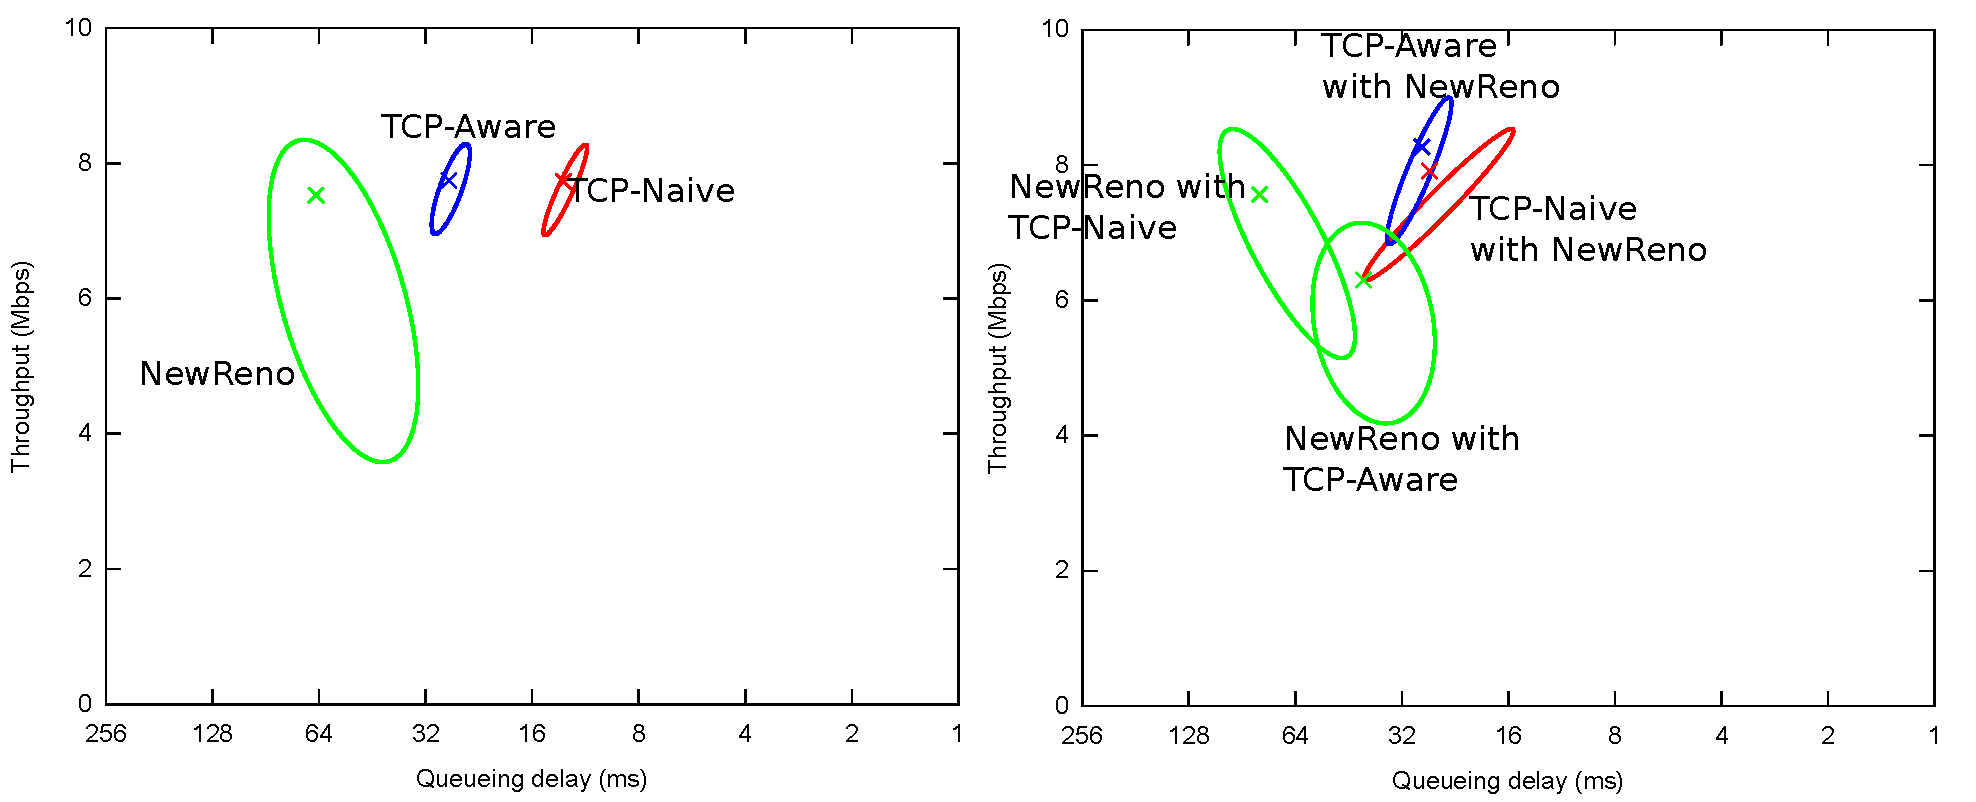
\includegraphics[width=\columnwidth]{compatible-5sec.pdf}
%\caption{TCP-Aware and TCP-Naive RemyCCs, 5 second ON/OFF}
%\end{subfigure}
%
%\begin{subfigure}[b]{\columnwidth}
\caption{RemyCCs designed with and without TCP-awareness,
  competing against themselves or against TCP. Shown here, two
  endpoints contending for a 10~Mbps link with 100~ms RTT, 250 kB of
  buffer capacity (200~ms maximum queueing delay), and
  almost-continuous offered load. The fair share of throughput is
  5~Mbps per endpoint. Ellipses show 1-$\sigma$ range of results.}
%\end{subfigure}
\begin{center}
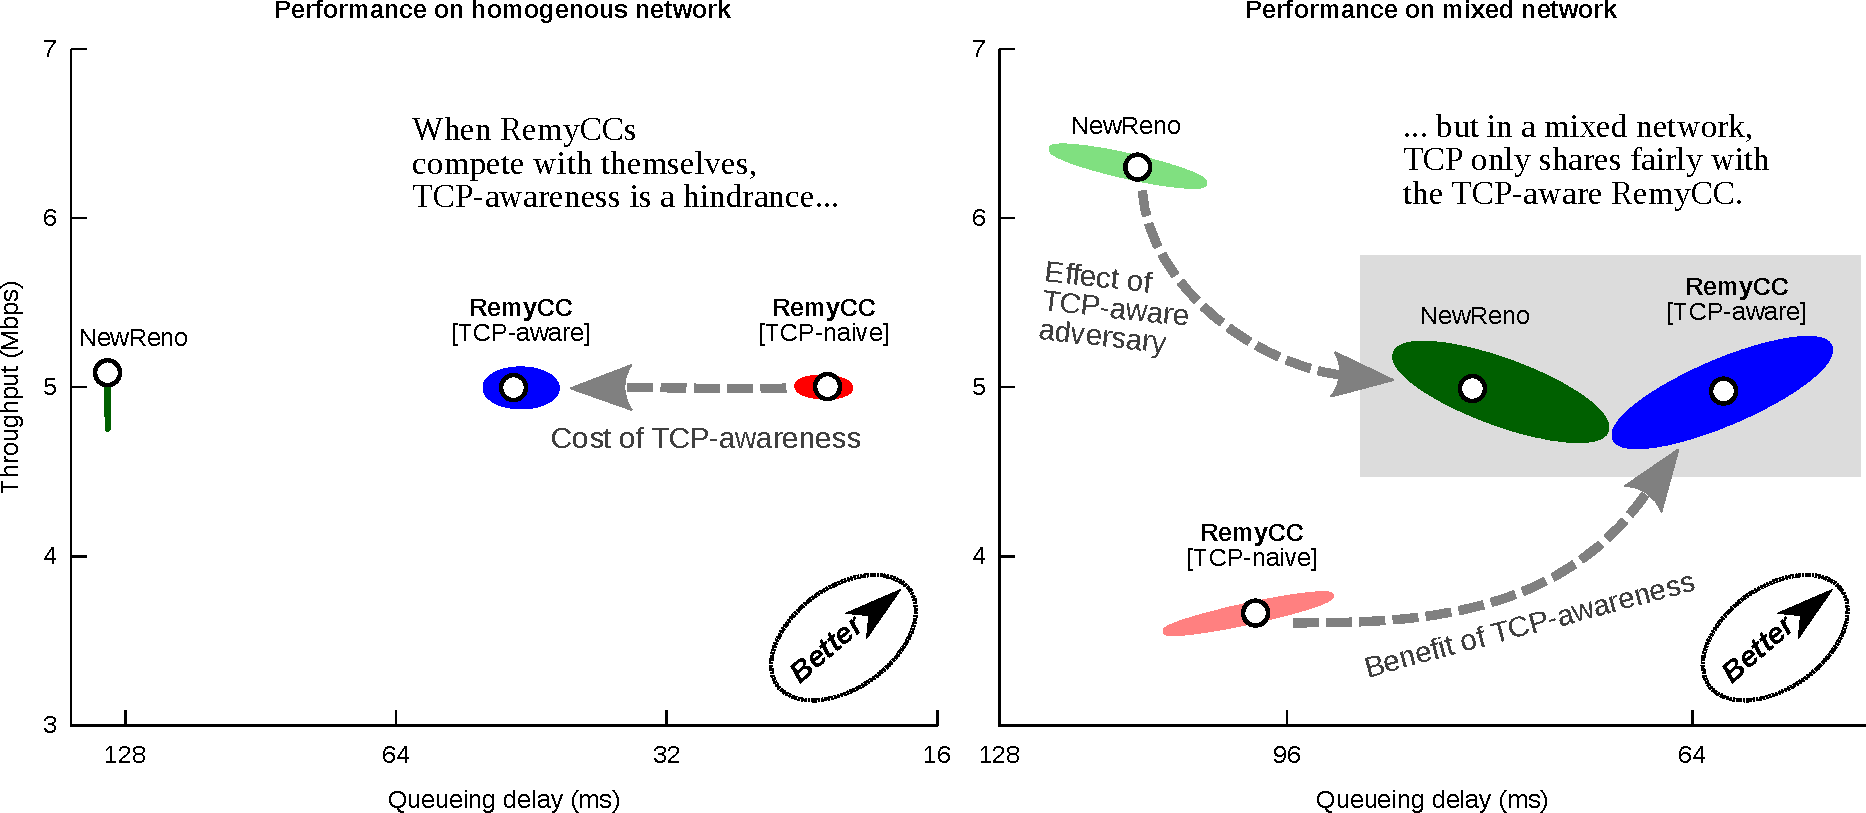
\includegraphics[width=\textwidth]{figures/manual/compatibility-drawn.pdf}
\end{center}
\label{fig:tcpaware}
\end{figure}
\end{comment}

\label{s:tcpaware}

We investigated the consequences of designing a congestion-control
protocol with the knowledge that some cross-traffic may be the product of
pre-existing incumbent protocols.

This question has considerable practical relevance: outside of an internal network controlled by a small number of parties, the
developer of a new network protocol will rarely be able to arrange a
``flag day'' when all endpoints switch to the new
protocol.\footnote{There has not been a ``flag day'' on the Internet
  since the switch to IP in 1983.}

On the broad Internet today, cross-traffic will typically be the
product of traditional loss-triggered TCP congestion-control
protocols, such as NewReno or Cubic. This status quo presents a
problem for new protocols that seek to perform differently or
that try to avoid building up standing queues inside the network.

Some protocols, such as Vegas~\cite{vegas}, perform well when
contending only against other flows of their own kind, but are
``squeezed out'' by the more-aggressive cross-traffic produced by
traditional TCP. Conventional wisdom is that any ``delay-based''
protocol will meet a similar fate. This has contributed to a lack of
adoption of Vegas and other delay-based protocols.

Ideally, a newly-designed protocol would perform well (e.g.~high
throughput, low delay) when interacting with other endpoints running
the same protocol, \textbf{and} would appropriately share a network
with incumbent endpoints running traditional TCP. But what are the
consequences of building this ``TCP-awareness'' into a protocol?

We studied this by designing two network protocols for a simple
network---one whose model specified that the cross-traffic would be
from the same protocol, and one whose model included a training
scenario where the cross-traffic was from traditional TCP half the
time.

\begin{figure}
\caption{Performance of two flows of the same congestion-control
  scheme contending for a 10~Mbps link, for three different
  congestion-control schemes. The ``TCP-naive'' RemyCC is designed
  under the assumption that its competition, when present, is governed
  by the same RemyCC---an assumption that holds here. The
  ``TCP-aware'' RemyCC is designed under the assumption that its cross
  traffic has a 50\% chance of being governed by a TCP AIMD-like
  scheme. The results quantify the degree to which designing a
  protocol to play well with TCP can exact a cost when TCP is absent.}
\label{fig:tcphomog}
\begin{center}
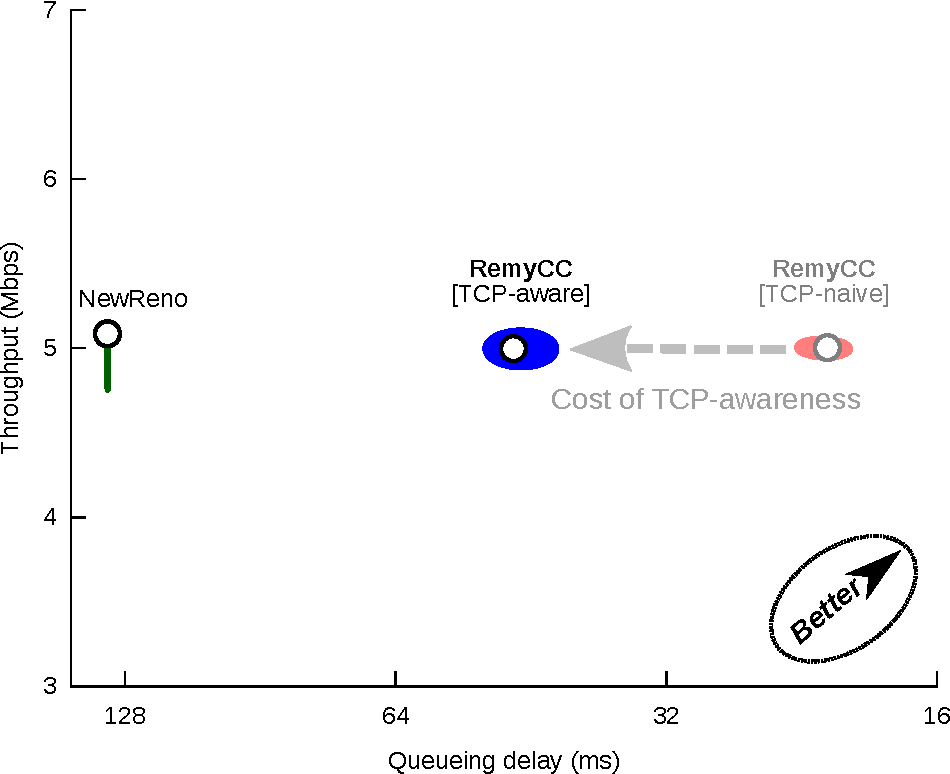
\includegraphics[width=\textwidth]{homo-3.pdf}
\end{center}
\label{fig:tcpawarehomo}
\end{figure}

\begin{figure}
\caption{When cross traffic is governed by TCP NewReno, the TCP-aware
  RemyCC achieves a more equitable division of the link---and better
  delay for both flows---than the TCP-naive RemyCC. The results
  demonstrate the benefit of TCP-awareness when TCP is present.}
\label{fig:tcpheterog}
\begin{center}
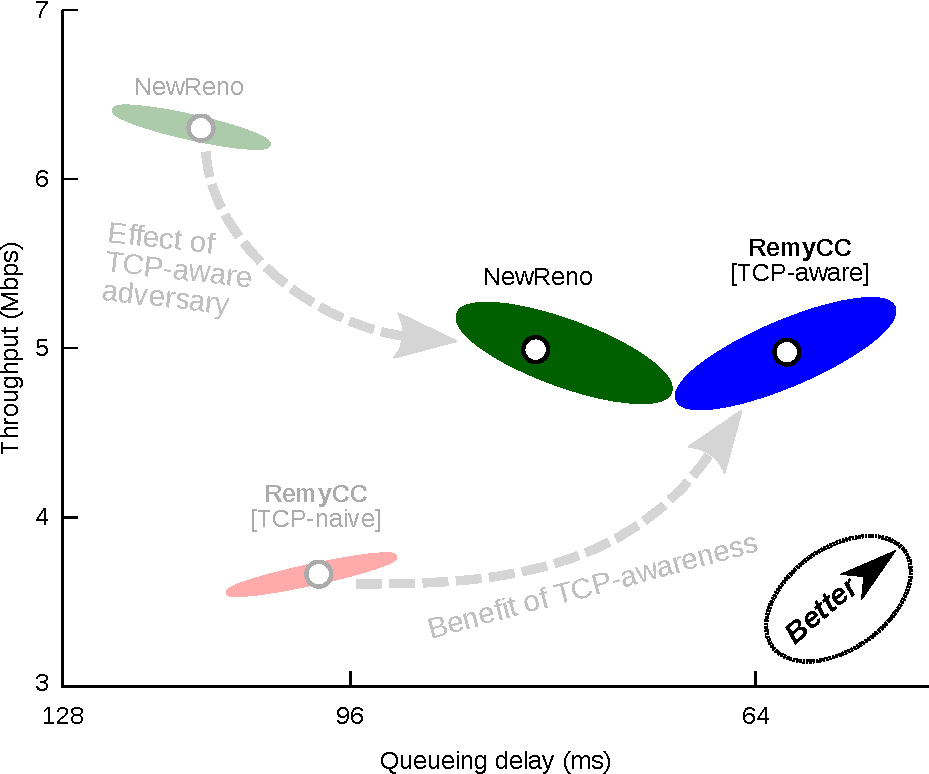
\includegraphics[width=\textwidth]{hetero-3.pdf}
\label{fig:tcpawarehetero}
\end{center}
\end{figure}

In Figure~\ref{fig:tcphomog}, protocols compete only with
cross-traffic from the same protocol. In this homogeneous setting,
adding TCP-awareness to a RemyCC builds up standing queues, more than
doubling the queueing delay without affecting throughput.

But in a mixed setting (Figure~\ref{fig:tcpheterog}) where a RemyCC
competes against TCP NewReno, the TCP-naive RemyCC is squeezed out and
does not get its fair share of the link. In the shaded region showing
the results when NewReno competes with the TCP-aware RemyCC,
TCP-awareness allows the RemyCC to claim its fair share of the link
and reduces the queueing delay experienced both by itself and by TCP
NewReno.

The results indicate that new delay-minded protocols \emph{can} avoid
being squeezed out by traditional loss-triggered TCP, but building in
this behavior comes at a cost to performance in the absence of TCP
cross-traffic.


\section{Congestion Control in a Diverse World}
%% Is coping too weak of a term?
\label{s:diversity}

In \S\ref{s:tcpaware}, we discussed the costs and benefits of
TCP-awareness. Here we report on further investigations to understand
the differing performance of TCP-naive and TCP-aware Tao protocols by
inspecting their transmissions in the time domain, when contending
with TCP cross-traffic (Figure~\ref{fig:explain}). The results show
that TCP-awareness is a complicated phenomenon, which yields higher
delays in isolation but smaller delays when contending with TCP. It is
not simply a question of ``more aggressive'' or ``less aggressive''
congestion-control.

\begin{figure*}
\centering
\begin{subfigure}[b]{0.4\textwidth}
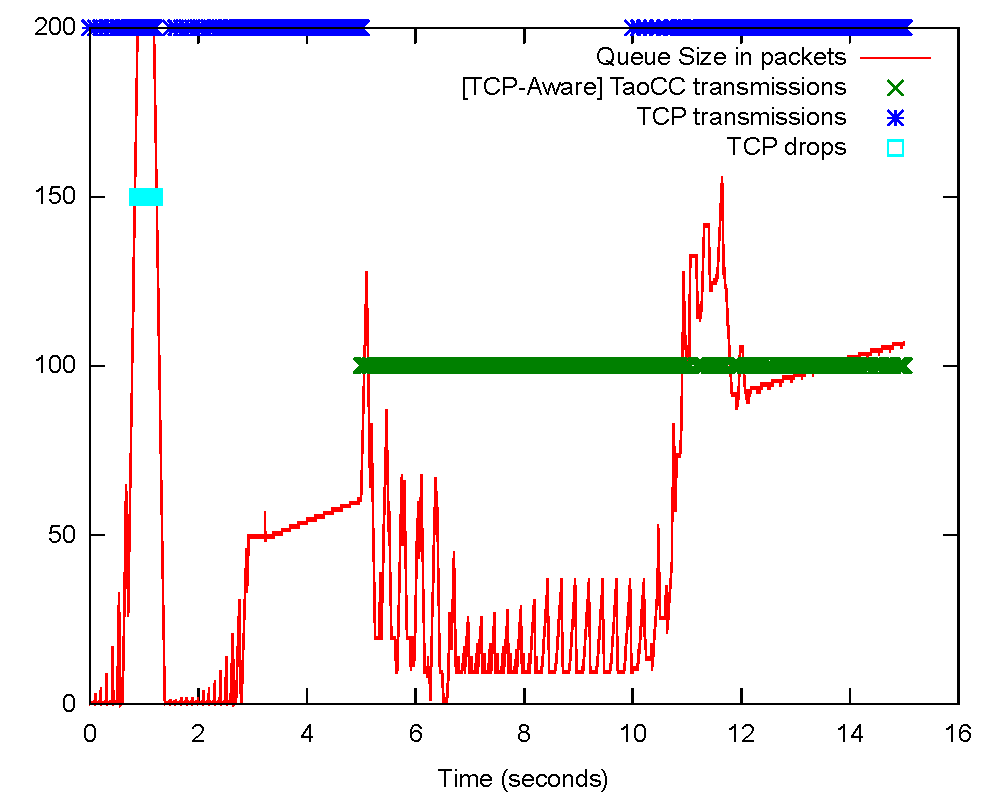
\includegraphics[width=\textwidth]{tx-queue-aware.pdf}
\end{subfigure}
\begin{subfigure}[b]{0.4\textwidth}
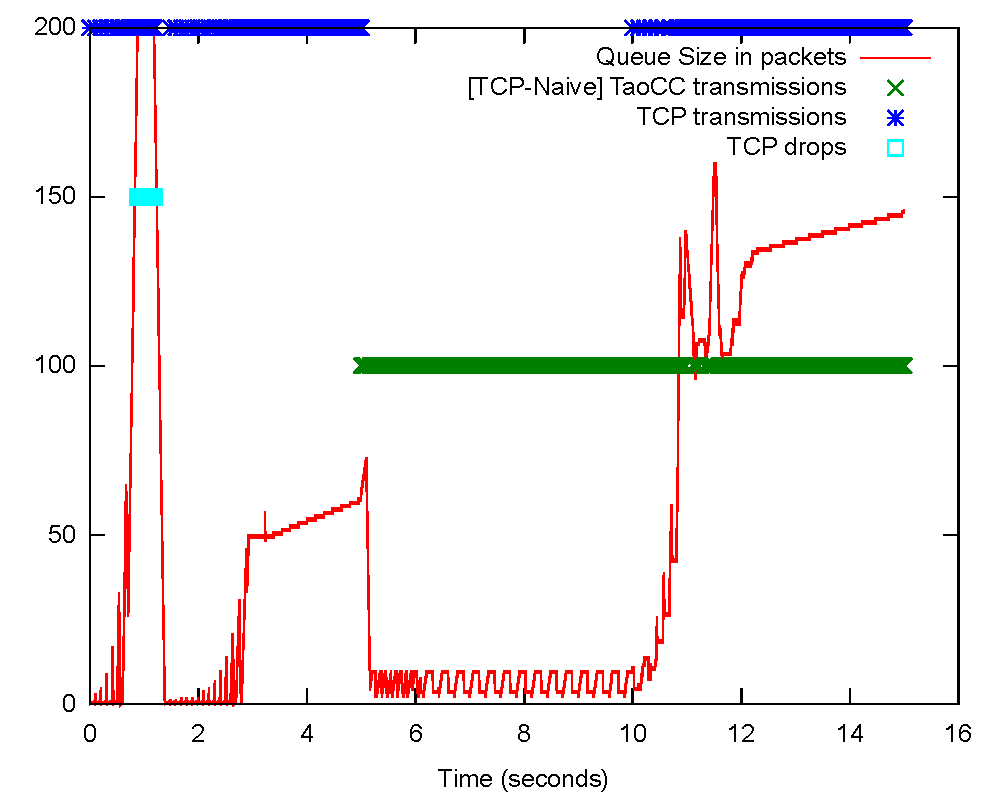
\includegraphics[width=\textwidth]{tx-queue-naive.pdf}
\end{subfigure}
\caption{In isolation, a TCP-aware Tao protocol is more aggressive than it needs to be, leading to higher delays. But when competing with TCP cross-traffic, the Tao protocol achieves the reverse situation---lower queueing delay, and higher throughput, than the TCP-naive Tao protocol.}
\label{fig:explain}
\end{figure*}


\label{ss:backward}

\subsection{The price of sender diversity}
\label{ss:forward}

\begin{figure}
\centering
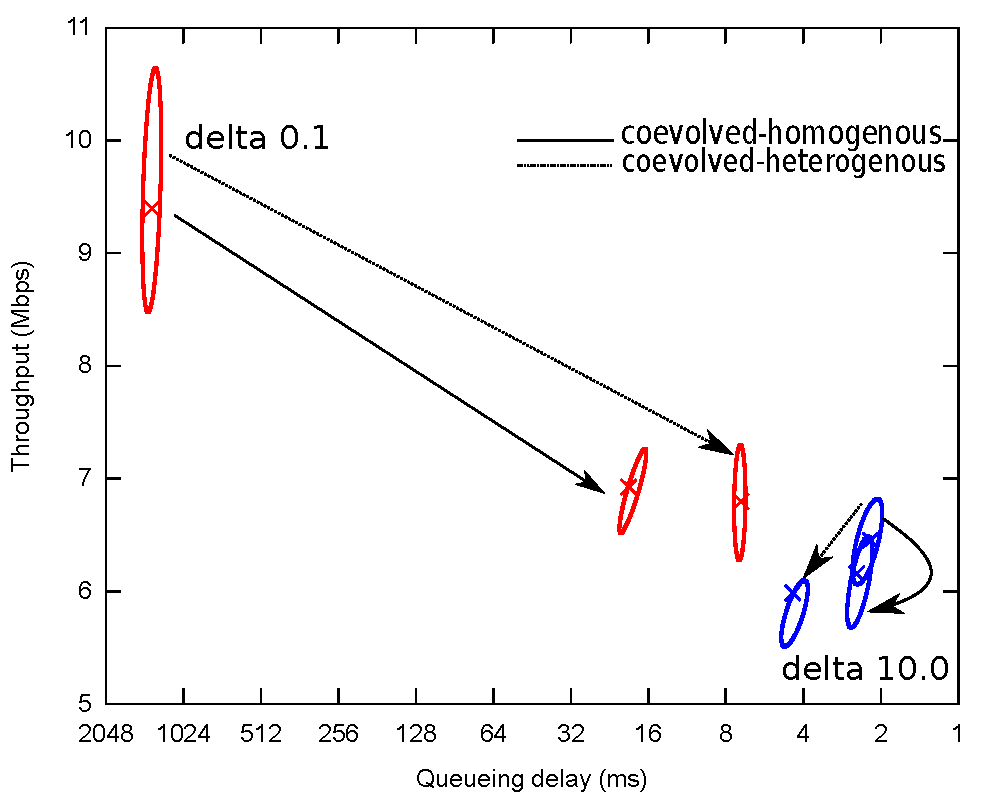
\includegraphics[width=\columnwidth]{diversity-both.pdf}
\caption{Co-designing Tao protocols for differing objectives brings both protocols towards a middle ground, but preserves some room for diversity.}
\label{fig:diversity-training}
\end{figure}

We further generalize the notion of TCP-awareness by asking whether it
is possible to design multiple new congestion-control protocols to
simultaneously achieve differing objection's when contending on the
same bottleneck link.

We investigate the possibility of co-developing congestion-control protocol
for differing sender objectives. We consider two extreme cases: a sender
that weighs throughput ten times over delay ($\delta=0.1$), and a sender that
weighs delay ten times over throughput ($\delta=10.0$).

We suspected that achieving diversity in this manner may not be
possible, reasoning that endpoints that share the same bottleneck link
will necessarily experience the same queueing delay, and therefore
endpoints that achieve an optimal throughput-to-delay tradeoff will
experience the same overall performance.

But contrary to this hypothesis, our findings are that it is possible
to co-develop congestion control algorithms such that they can both
co-exist with each other and yet---because of variable duty
cycles---achieve some diversity in their chosen objectives.  Even when
running together, the delay-preferring sender sees lower delay than
the throughput-preferring sender, while the opposite is true with
throughput. When congestion-control protocols are co-developed, but
each sender runs homogeneously, each sender receives higher throughput
or lower delay, as the case they may be.

However, coexistence does come at a price to the throughput-preferring
sender, which suffers a loss in throughput by being ``nice" to the
delay-preferring sender. By comparison, the performance of the
delay-preferring sender is affected only modestly.

\section{Conclusion}
\label{s:concl}

In the context of network congestion control, we asked: How faithfully
do protocol designers really need to understand the networks they
design for? What are the important signals that endpoints should
listen to?  How can researchers gain confidence that systems that work
in testing scenarios will also perform adequately on real networks
that are inevitably more complex, or future networks yet to be
developed? Is there a tradeoff between the performance of a protocol
and the breadth of its intended operating range of networks?  What is
the cost of playing fairly with cross-traffic that is governed by
another protocol?

We examined these questions using Remy as a design tool to produce a
tractable attempt at optimal (Tao) protocol under various
conditions. We found only weak evidence of a tradeoff between
operating range and performance, even when operating range was
extended to cover a thousand-fold range of link rates. We found that
it may be acceptable to simplify some characteristics of the
network---such as its topology---when modeling for design
purposes. Some other features, such as the degree of multiplexing and
the aggressiveness of contending endpoints, are important to
capture. These results may provide useful insights to network protocol
designers about what factors are important to model accurately and
what factors may be simplified.


\chapter{Mosh}
\label{chap:mosh}

\chapter{Critiques \& Conclusion (XXX TBA)}

%\appendix
%\chapter{Tables}

\begin{table}
\caption{Armadillos}
\label{arm:table}
\begin{center}
\begin{tabular}{||l|l||}\hline
Armadillos & are \\\hline
our	   & friends \\\hline
\end{tabular}
\end{center}
\end{table}

\clearpage
\newpage

%\chapter{Figures}

\vspace*{-3in}

\begin{figure}
\vspace{2.4in}
\caption{Armadillo slaying lawyer.}
\label{arm:fig1}
\end{figure}
\clearpage
\newpage

\begin{figure}
\vspace{2.4in}
\caption{Armadillo eradicating national debt.}
\label{arm:fig2}
\end{figure}
\clearpage
\newpage

%% This defines the bibliography file (main.bib) and the bibliography style.
%% If you want to create a bibliography file by hand, change the contents of
%% this file to a `thebibliography' environment.  For more information 
%% see section 4.3 of the LaTeX manual.
\begin{singlespace}
\bibliography{main}
\bibliographystyle{abbrv}
\end{singlespace}

\end{document}
